\chapter{Initial Muon Neutrino Charged Current Inclusive Measurement} \label{sec:FistCCInclusive}
In 2016, I was a vital part of MicroBooNE's first \gls{cc} inclusive measurement, published in a public note \cite{MicroBooNECCInclPN} in the same year. Thereafter, I developed the analysis further, resulting in the work presented in this chapter. Since it was the first analysis, only a couple of months after detector commissioning, the results sparked many improvements in the reconstruction and simulation chain alike. The analysis also marked the basis for MicroBooNE's first peer-reviewed \gls{cc} inclusive cross section paper \cite{MicroBooNEFirstCCInclPublished} and some of the selection cuts developed here are now used in the pre-selection process.  

In this chapter, I will first, give an overview of the software tools used in this analysis. Then, the data and \gls{mc} samples are introduced, followed by a description of the reconstruction processes of the raw light and charge signals. Thereafter, the selection process I developed is outlined and finally the results are presented.

\section{Software Tools and Simulation} \label{sec:SoftwareTools}
The software tasks of \gls{mc} simulation, event reconstruction, and event selection are all handled by the \gls{LArSoft} toolkit developed at \gls{fnal} \cite{LArSoftWeb,LArSoft}. \Gls{LArSoft} is written in the \cpp programming language and structurally rests upon the \gls{art} \cite{ARTWeb,ART}. \Gls{art}, and hence \gls{LArSoft}, is an event-processing framework. In MicroBooNE, an event contains all the data collected during three \gls{tpc} readout windows around a trigger signal. Now, \gls{art} loops through these events and allows the user to interact with the collected event data. The interaction with the event data is achieved via so-called modules. There are three different module types available for the common user: \textbf{Producer}, \textbf{Filter}, and \textbf{Analyzer}. The Producer adds data products to the events, which is useful for \ia reconstruction tasks. The Filter is used to remove data products or events from the data sample, which is used \ia for selection code. The Analyzer, does not change the event data and is only used to extract and analyse the event information \cite{ART}. In this analysis, the Analyzer module was only used to generate a ROOT file, in order to produce plots outside of \gls{LArSoft}. 

\Gls{LArSoft} makes also use of various other software libraries and tools besides \gls{art}. For \gls{mc} sample generation, \gls{LArSoft} employs \gls{genie} \cite{GenieGenerator,GenieTools} as neutrino generator. \Gls{genie}, uses the neutrino beam flux (see figure \ref{fig:BNBFlux}) as an input and provides neutrino interaction \gls{Vertex} information of the interaction products, like: position, momentum, and particle type. Cosmic-ray particle events are generated by \gls{corsika} \cite{CorsikaWeb,Corsika}. \Gls{corsika} outputs position, momentum and energy for cosmic-ray particles, similar to \gls{cry} in the aforementioned cosmic gamma-ray background study presented in chapter \ref{sec:CosmicRayGammaBackground}. All the generator information is then first processed through \gls{geant} \cite{MCSimulationGeant4}, simulating the particle's passage through matter. From there, \gls{LArSoft}-specific code simulates the relevant \gls{lartpc} processes: recombination and scintillation (see section \ref{sec:RecombAndScint}), \gls{quasifreeelectron} drift (see section \ref{sec:ChargeDrift}), as well as the charge, and light readout (see sections \ref{sec:ChargeReadout} and \ref{sec:LightReadoutSystems}, respectively). Finally, \gls{LArSoft} also simulates the electronics response, with the aim of modelling the real detector as accurately as possible. Ideally, the \gls{mc} samples and the raw data should be indistinguishable at this point, in order to make the samples compatible. In reality, this feat is almost impossible to accomplish and the simulation deficiencies have to be expressed as systematic uncertainties. Data and \gls{mc} sample reconstruction are either handled by \gls{LArSoft}'s own algorithms or by the \gls{Pandora} software kit for pattern recognition purposes \cite{Pandora,PandoraLAr}. As this description implies, \gls{Pandora} is used to identify and reconstruct the charge signal, produced by particle tracks and showers in the MicroBooNE \gls{lartpc}. A more detailed description of \gls{Pandora} will follow in section \ref{sec:EventReconstruction}. As mentioned before, the data analysis is then performed by ROOT \cite{ROOT}.

The \gls{mc} samples were generated using \gls{LArSoft} v04.36.00, more precisely, a MicroBooNE tailored version called \textbf{uboonecode} v04.36.00, which makes use of the generators listed below. The reconstruction of the \gls{mc} and \gls{tpc} data samples was performed with \gls{LArSoft} v05.08.00, \ie \textbf{uboonecode} v05.08.00, and its respective \gls{Pandora} version. The used \gls{LArSoft} version and the versions of its relevant tools are listed below \cite{MicroBooNECCInclPN}.
\begin{outline}
    \1 \gls{LArSoft} v04.36.00 (\gls{mc} Simulation)
        \2 \gls{genie} v2.8.6 (baseline model)
        \2 \gls{genie} v2.10.6 (additional models)
        \2 \gls{corsika} v7.4003
        \2 \gls{geant} v4.9.6.p04d
    \1 \gls{LArSoft} v05.08.00 (all reconstruction)
        \2 \gls{Pandora} v2.3.0a
\end{outline}

\section{TPC Data Samples} \label{sec:DataSamples}
The data taking period for this analysis ranges from February 23, 2016, to May 22, 2016 (MicroBooNE run numbers \num{5212} to \num{6356}). The beginning of this data set marks the switch to data taking utilising the light readout system for triggering, which reduces the data rate by about a factor of \num{20}. The trigger, simply called \gls{bnb} trigger, is applied in software and requires a minimum amount of scintillation light observed during the beam window, \ie \gls{BeamGate}, of \SI{1.6}{\micro\second} length, integrated over all \glspl{pmt}. Two different \gls{tpc} data streams are utilised for this analysis. One is the data stream delivering \textbf{on-beam} data, for which a \gls{bnb} \gls{BeamGate} trigger and a scintillation \gls{Flash} have to coincide, as mentioned in section \ref{sec:MicroBooNEReadout}. The other is the \textbf{off-beam} data stream, which is taken with the exact same trigger settings as the on-beam data, but during periods when no beam was received. This is achieved by introducing an external fake \gls{BeamGate} in coincidence with a real \gls{Flash} signal. This external trigger setup is referred to as \textbf{BNBEXT}. The off-beam data set is used here as a data-driven measurement of cosmic background \cite{MicroBooNECCInclPN}.

In order to ensure reliability and comparability of the data sets, a so-called \textbf{good run} list had to be compiled. Good runs, during this period, were selected taking into account successful operation in all relevant areas: 
\begin{itemize}
    \item \textbf{Beam conditions}: stable \gls{bnb} metrics 
    \item \textbf{Detector conditions}: stable metrics of all detector subsystems
    \item \textbf{Data quality}: basic reconstruction quantities show stable behaviour
\end{itemize}
The beam conditions are observed with three variables. One of them is the so-called \gls{fom} which measures the fraction of protons in a beam pulse hitting the target, \ie full beam on target \gls{fom} $ = 1$, no beam on target \gls{fom} $ = 0$. For this analysis the condition \gls{fom} $ > 0.95$ is used. Another condition is the proton collision yield of at least \num{0.5e12} \gls{pot} per beam pulse. This limit allows for ten times lower \gls{pot} values than expected during normal \gls{bnb} operations (see section \ref{sec:BNB}). The last beam variable determining the data quality, is the horn current. A good run has to feature stable horn currents between \SIlist{172;176}{\kilo\ampere} \cite{MicroBooNEBeamStabilityIN}. The detector stability is determined by seven different subsystems, many of which feature multiple monitored variables shown in brackets. These include the front end \gls{asic} voltage supplies (\num{42} variables), the \gls{daq} crate power rails (\num{22}), \gls{daq} status (\num{18}), \gls{tpc} wire bias voltage (\num{38}), and \gls{pmt} \gls{hv} (36). The missing two variables are the \gls{tpc} drift \gls{hv}, expected between \SIlist{70.1;96.7}{\kilo\volt}, and the \gls{quasifreeelectron} lifetime with the lower limit of \SI{2}{\milli\second} \cite{MicroBooNEDetectorStabilityIN}. Finally, the data quality is checked by monitoring the number of reconstructed tracks, \glspl{Vertex}, and \glspl{Flash} $ > 50$ \gls{pe}, each averaged on an event basis. The distribution of each of these quantities over all runs was fitted to a Gaussian curve and runs lying within $3\sigma$ bounds of the fitted Gaussian distribution in both data streams were selected \cite{MicroBooNEDetectorStabilityPN}. Furthermore, a \SI{100}{\percent} success rate during the data processing was required. In summary, a fraction of \SI{91.7}{\percent} of the delivered \gls{pot} from the \gls{bnb} passed all criteria mentioned above \cite{MicroBooNECCInclPN}.

In order to comply with the MicroBooNE data blindness policy, the open data sample for the \gls{bnb} on-beam stream is further downsized to not exceed a total of \num{4.95e19} \gls{pot}. Therefore, the on-beam sample used here ends on April 17 with run 5946, which adds up to a total of \num{4.95e19} \gls{pot} \cite{MicroBooNEBeamStabilityIN}. For the off-beam sample the entire period is used. The number of recorded events, $N^\text{Trig}_\text{BNB}$ for on-beam and $N^\text{Trig}_\text{EXT}$ for off-beam, as well as the total number of \glspl{BeamGate} received by the trigger board, $N^\text{Gate}_\text{BNB}$ for on-beam and $N^\text{Gate}_\text{EXT}$ for off-beam, are shown in table \ref{tab:DataSamples}.
\begin{table}[htbp]
    \centering
    \caption[Detector Data Samples Used in the CC Inclusive Analysis]{These are the recorded data samples used in this \gls{cc} inclusive cross section analysis. $N^\text{Trig}$ stands for the total number of recorded events, \ie number of \gls{Flash} plus \gls{BeamGate} triggers received, and $N^\text{Gate}$ for the number of \gls{BeamGate} only triggers received (either \gls{bnb} or \textbf{BNBEXT}).}
    \begin{tabu}{llrrr}
        \toprule
        \rowfont[c]{\bf} Sample name & Trigger & $N^\text{Trig}$ & $N^\text{Gate}$ & \gls{pot} \\
        \midrule
        on-beam & \gls{bnb} & \num{546910} & \num{11045346} & \num{4.95e19} \\
        off-beam & \textbf{BNBEXT} & \num{388471} &  \num{8979753} & \multicolumn{1}{c}{N/A} \\
        \bottomrule
        \label{tab:DataSamples}
    \end{tabu}
\end{table}

As mentioned before, the off-beam sample serves as cosmic background measurement. More specifically, it is a reducible cosmic background which produces a \gls{Flash} trigger signal in a \gls{BeamGate} with no neutrino interaction. In order to make the two data sets directly comparable, said off-beam sample needs to be scaled. In this case, the scaling factor can be extracted from the rate of flashes, $R^\text{Flash}$, of the two data samples:
\begin{align} \label{eq:BNBFlashRate}
    R^\text{Flash}_\text{BNB} &= R^\text{Flash}_\nu + R^\text{Flash}_\text{BGR} = \frac{N^\text{Trig}_\text{BNB}}{N^\text{Gate}_\text{BNB}}, \\
    R^\text{Flash}_\text{EXT} &= R^\text{Flash}_\text{BGR} = \frac{N^\text{Trig}_\text{EXT}}{N^\text{Gate}_\text{EXT}}.
    \label{eq:EXTFlashRate}
\end{align}
In above equation $R^\text{Flash}_\nu$ stands for the \gls{Flash} rate introduced by neutrino, and $R^\text{Flash}_\text{BGR}$ the rate of cosmic background interactions, respectively. As can be seen, one can expect the same cosmic background \gls{Flash} rate for both data samples. We can thus replace $R^\text{Flash}_\text{BGR}$ of equation \ref{eq:BNBFlashRate} with the relation found in equation \ref{eq:EXTFlashRate} and solve for the neutrino related flash rate,
\begin{align}
    R^\text{Flash}_\nu &= \frac{N^\text{Trig}_\text{BNB}}{N^\text{Gate}_\text{BNB}} - \frac{N^\text{Trig}_\text{EXT}}{N^\text{Gate}_\text{EXT}} \nonumber \\
    \Longrightarrow \ N^\text{Gate}_\text{BNB} R^\text{Flash}_\nu &= N^\text{Trig}_\nu = N^\text{Trig}_\text{BNB} - \frac{N^\text{Gate}_\text{BNB}}{N^\text{Gate}_\text{EXT}} N^\text{Trig}_\text{EXT}.
    \label{eq:NumberOfNu}
\end{align}
By multiplying the neutrino flash rate, $R^\text{Flash}_\nu$, by the number of \gls{bnb} \glspl{BeamGate}, $N^\text{Gate}_\text{BNB}$, we received the number of neutrino induced trigger events, $N^\text{Trig}_\nu$, in the last step of above equation. Moreover, we obtained the proper scaling factor for the off-beam sample in the process, given by $N^\text{Gate}_\text{BNB} / N^\text{Gate}_\text{EXT}$. Using the numbers listed in table~\ref{tab:DataSamples} we get $N^\text{Gate}_\text{BNB} / N^\text{Gate}_\text{EXT} = \num{1.23}$ for the scaling factor, and $N^\text{Trig}_\nu = \num{69091}$ total neutrino event triggers.

\section{Monte Carlo Samples} \label{sec:MCSamples}
In this analysis, four simulated \gls{bnb} samples and one cosmic-ray sample are used. The neutrino \gls{mc} samples serve three purposes. They are used to optimise cuts in the selection process, which will be outlined in more detail in section \ref{sec:EventSelection}. Furthermore, they deliver estimates for the irreducible backgrounds and with it selection efficiencies and purities. Lastly, they provide model comparisons to the \gls{tpc} data sets of the actual measurement introduced before in section \ref{sec:DataSamples}. Moreover, the cosmic sample serves the purpose of a quality check on the cosmic simulation chain and provides an estimate for systematic uncertainties for the irreducible cosmic-ray muon background, see section \ref{sec:Systematics}. In order to achieve these purposes, all \gls{mc} samples must bare strong resemblance to real \gls{tpc} data, to such a degree, that they behave the same way during reconstruction and selection. For this, as mentioned in section \ref{sec:SoftwareTools}, \gls{LArSoft} simulates all relevant detector behaviour introduced in chapter \ref{sec:LArTPC} as well as electronics responses. 

The cosmic-ray sample is the \gls{mc}-equivalent to the off-beam data set, for it features a \gls{BeamGate} \gls{Flash} and consists of pileup cosmic background events (see section \ref{sec:CosmicPileup}). Hence, these cosmic-ray events, generated by \gls{corsika}, scales linearly to $N_\text{Trig}^\text{EXT}$ by the number of events in the sample. The \gls{bnb} \gls{mc} samples, however, are not directly comparable to the on-beam data set, since they features a neutrino interaction in every single event. But they are comparable with $N_\text{Trig}^\nu$, derived in equation \ref{eq:NumberOfNu}. Therefore, they scale linearly to $N_\text{Trig}^\nu$ by their respective number of \gls{pot}. Thus, in order to directly compare an \gls{mc} sample to $N_\text{Trig}^\nu$, it has to be scaled by $N_\text{POT}^{Data}/N_\text{POT}^{MC}$.

% TODO Referre to axial mass in the theory?
The \gls{bnb} \gls{mc} samples all use a different neutrino interaction model. First there is the \gls{genie} v2.8.6 \textbf{Baseline} model with an axial mass $M_A=\SI{0.99}{\giga\electronvolt}$. It serves as reference model for the selection optimisation and for the irreducible background estimates. The three other interaction models, generated using \gls{genie} v2.10.6, are \cite{MicroBooNECCInclPN}:
\begin{itemize}
    \item Axial vector mass for quasi-elastic interactions: At high neutrino energies a \gls{rfg} model of the nucleus, and a dipole axial form factor with axial mass of approximately \SI{1}{\giga\electronvolt}, was found to agree well with data. In observations of \gls{ccqe} events at MiniBooNE \cite{AxialMassMiniBooNE}, this model was found to not agree well with the data, and fits resulted in an ``effective'' axial mass value of \SI{1.35}{\giga\electronvolt}. Here we modify the axial vector mass from the \gls{genie} baseline value of $M_A = \SI{0.99}{\giga\electronvolt}$ to $M_A = \SI{1.35}{\giga\electronvolt}$ by re-weighting the \gls{genie} baseline simulation \cite{GenieTools}. The primary effect of the axial mass increase is an increase in normalisation. The effect on the total number of expected selected events is of the order of \SI{24}{\percent}.
    \item Effective spectral functions with transverse enhancement: \gls{tem} \cite{CrossSectionModelTEM} is another way to model the nuclear effects. In this model, the transverse cross-section is enhanced based on the observation in the electron scattering data. The empirical superscaling function is modeled with the \gls{esf} \cite{CrossSectionModelESF}. The \gls{esf} replaces the \gls{rfg} model which is used in all other samples as the \gls{genie} default. Only the lepton is affected by this - there is no impact on the hadronic side of the interaction. The effect on the total number of expected selected events is of the order of \SI{13}{\percent}.
    \item \gls{mec}: Rather than introducing an effective parameter, additional processes are proposed which would address the discrepancies seen in the MiniBooNE data. \gls{mec} are one way to model an additional process, where a neutrino interacts with a correlated pair of nucleons (which may be in a quasi-deuteron state). It is also often referred to as 2p2h, or multinucleon interactions. As the correlation between nucleons is mediated by the exchange of a \gls{Meson}, this process is known as \gls{mec}. The model referred to as \gls{mec} in the following plots is a microscopic model for \gls{mec} by Nieves \emph{et al}. \cite{CrossSectionModelMEC}. The effect on the total number of expected selected events is of the order of \SI{24}{\percent}.
\end{itemize}
Naturally, all four \gls{bnb} \gls{mc} samples feature simulated cosmic pileup events provided by \gls{corsika} to resemble \gls{pmt} data neutrino events. The cosmic-ray only \gls{mc} sample is called \textbf{inTime cosmic}. All samples and their respective (\gls{pot}) scaling are listed in table \ref{tab:MCSamples}.
\begin{table}[htbp]
    \centering
    \caption[MC Samples Used in the CC Inclusive Analysis]{The \gls{mc} samples generated for this \gls{cc} inclusive cross section analysis.}
    \begin{tabu}{llrr}
        \toprule
        \rowfont[c]{\bf} Sample name & Generators & $N_\text{Trig}$ & \gls{pot} \\
        \midrule
        \gls{bnb} Baseline & \gls{corsika}, \gls{genie} v2.8.6 & \num{189380} & \num{2.30e20} \\
        \gls{bnb} \textbf{M\textsubscript{A}\num{1.35}} & \gls{corsika}, \gls{genie} v2.10.6 & \num{187342}  & \num{2.00e20} \\
        \gls{bnb} \gls{mec} & \gls{corsika}, \gls{genie} v2.10.6 & \num{199999} & \num{2.08e20} \\
        \gls{bnb} \gls{esf}\&\gls{tem} & \gls{corsika}, \gls{genie} v2.10.6 & \num{200000}  & \num{2.32e20} \\
        \textbf{inTime cosmic} & \gls{corsika} only & \num{4804} & \multicolumn{1}{c}{N/A} \\
        \bottomrule
        \label{tab:MCSamples}
    \end{tabu}
\end{table}

\section{Event Reconstruction} \label{sec:EventReconstruction}
The \gls{tpc} data and \gls{mc} samples were both reconstructed using \textbf{uboonecode} v05.08.00 which features \gls{Pandora} v2.3.0a. Generally, there are two raw signal types to reconstruct: the \gls{pmt} light readout signals and the charge readout wire signals. While the reconstruction of the latter is publicly well documented, the information about the former had to be extracted from various internal talks and notes \cite{MicroBooNEFlashRecoIT1,MicroBooNEFlashRecoIT2,MicroBooNECCInclIN}. The goal of the \gls{Flash} reconstruction is to provide a time dependent heat map of light activity in the $y$-$z$-projection of the MicroBooNE \gls{tpc}. Ideally, this map would allow for every \gls{Flash} to be matched to charge signal activity. The aim of the charge signal reconstruction, on the other hand, is to generate a full \gls{3d} image of the ionisation activity in the \gls{tpc}.

The scintillation light collected by MicroBooNE's primary light detection system (see section \ref{sec:MicroBooNELightDetection}) is reconstructed by \gls{LArSoft}, \ie \textbf{uboonecode}. Each \gls{pmt} provides two different output streams, as established in section \ref{sec:MicroBooNEReadout}: one for the high-gain channel ($\sim \num{20}$ \gls{adc} counts per \gls{pe}) and the other for the low-gain ($\sim \num{2}$ \gls{adc} counts per \gls{pe}) channel. The first step performed in the optical reconstruction is the merging of these two streams into a so-called \textbf{saturation-corrected} waveform which tries to correct saturating high-gain pulses by using information from the low-gain channel. Since this is a \gls{bnb} event related analysis, the saturation-corrected \gls{BeamGate} unbiased readout window, \ie the \SI{23.4}{\micro\second} long window opened by the \gls{BeamGate} trigger, is used to reconstruct \glspl{OpticalHit}. Each \gls{pmt}'s waveform is scanned for \glspl{OpticalHit} which are located by first applying a rolling-baseline estimation, in order to be less sensitive to possible fluctuations in the signal baseline. At this stage a threshold-based hit-reconstruction algorithm is applied, requiring pulses of a minimum area in order for an \gls{OpticalHit} to be reconstructed. Each reconstructed \gls{OpticalHit} is associated with a \gls{pmt} number, a time (with respect to the trigger time in microseconds), and a \gls{pe} count. Once, \glspl{OpticalHit} are reconstructed on all \num{32} \glspl{pmt}, the information from all \glspl{pmt} is combined into \glspl{Flash}, which are meant to represent interactions in the detector, as seen by the light readout system. Each reconstructed \gls{Flash} contains information about the total amount of light seen in the interaction, measured in \glspl{pe}, as well as the distribution of light across all \num{32} \glspl{pmt}, and the \gls{Flash}-time, with respect to the trigger time. \Glspl{Flash} are reconstructed by requiring a time coincidence of $\sim \SI{1}{\micro\second}$ between hits on all \glspl{pmt} \cite{MicroBooNECCInclIN}. The total \gls{pe} measured across all time-coincident \glspl{OpticalHit} is summed together and \glspl{Flash} are reconstructed if the amount of light is larger than \num{2} \gls{pe}. However, there is a difficulty posed by the slow component of the scintillation light which exhibits a lifetime of \SI{1.6}{\micro\second}, as discussed in section \ref{sec:RecombAndScint}. Hence, a safeguard is placed to avoid reconstructing pulses from late scintillation light, as independent \glspl{Flash}. Given a time-coincident group of \glspl{OpticalHit}, subsequent potential \glspl{Flash} are reconstructed as such only if their total \gls{pe} value is more than $\num{3}\sigma$ above the expected amount of light produced by late-scintillation photons. This condition is given by the total light in the early pulse and the exponential reduction of the late scintillation light. If this condition is not met, the subsequent surge in light is recognised as late-light from the preceding \gls{Flash}, and not reconstructed as an independent \gls{Flash}. Aforementioned condition for coincident \glspl{OpticalHit} to be categorised as \glspl{Flash} or late light is depicted in figure \ref{fig:FlashReconstruction}.
\begin{figure}[htbp]
    \centering
    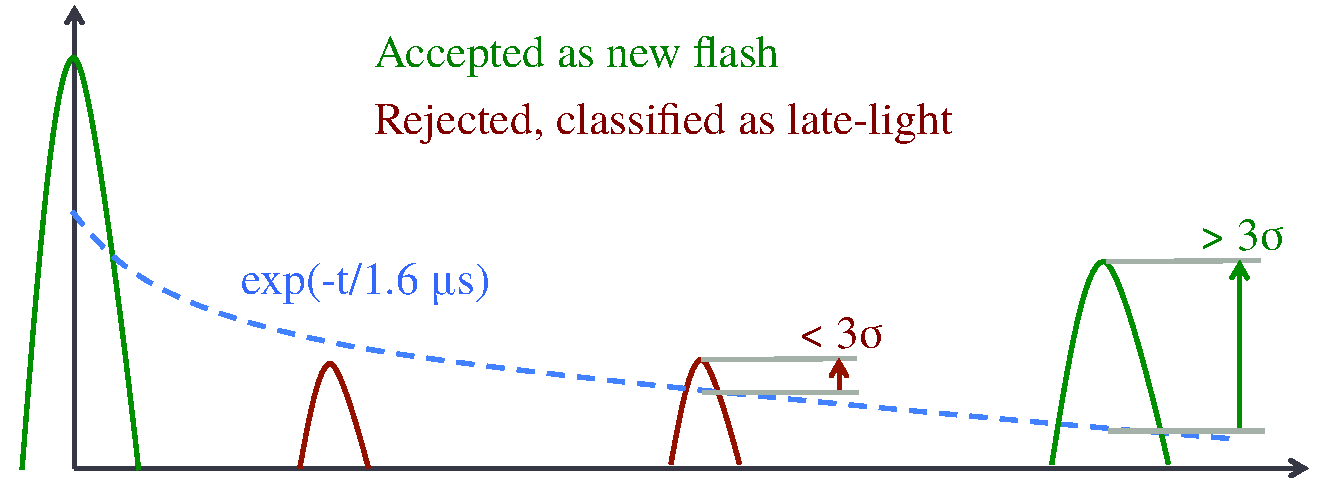
\includegraphics[width=1.0\textwidth]{images/FirstCCInclusive/FlashReconstruction.pdf}
    \caption[Flash or Late Scintillation Light Discrimination]{Shown here is a visual representation of the \gls{Flash} - late scintillation light safeguard discrimination algorithm. This graph is sourced and adapted from \cite{MicroBooNEFlashRecoIT1}.}
    \label{fig:FlashReconstruction}
\end{figure}
Moreover, a time distribution of optical \glspl{Flash}, reconstructed using \gls{bnb} unbiased-triggered events in which a clear excess in coincidence with the expected arrival time of neutrinos is expected, can be found in figure \ref{fig:BNBFlashes}. The information shown in this graph was produced with the same \gls{Flash} reconstruction tools used in this thesis, and serves as validation for this reconstruction tool. The thus reconstructed \gls{Flash} information, is stored in the \textbf{OpFlashSat} data product, an acronym for optical \gls{Flash} saturation-corrected.
\begin{figure}[htbp]
    \centering
    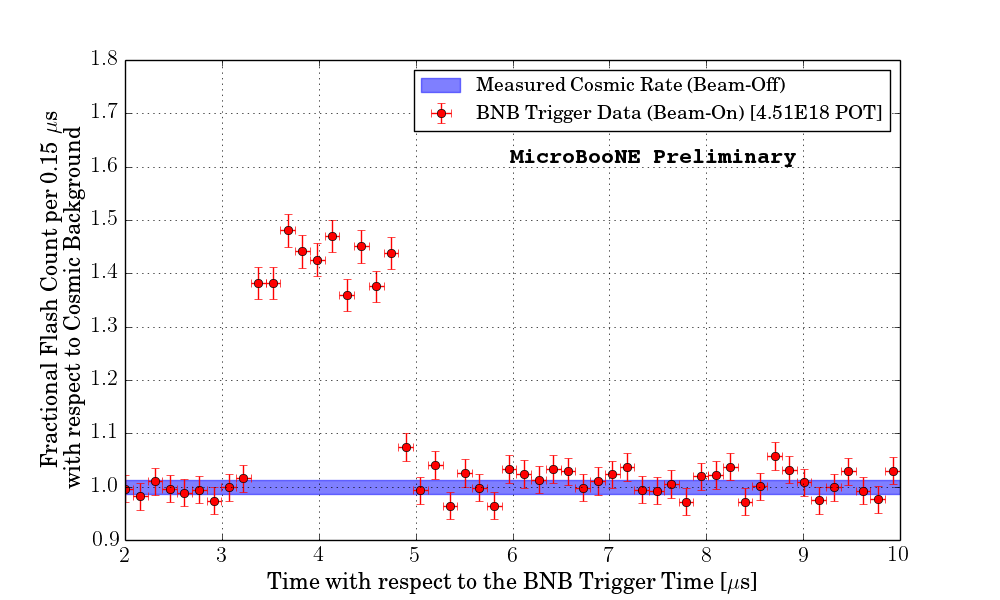
\includegraphics[width=0.9\textwidth]{images/FirstCCInclusive/BNBFlashes.png}
    \caption[Time Distribution of Reconstructed Optical Flashes]{Time distribution of reconstructed optical \glspl{Flash} with a \gls{pe} value of \num{50} or more (no optical trigger applied). A clear excess in coincidence with the \gls{bnb} pulses is observed. The passing rate for a \num{50} \gls{pe} threshold for the on-beam stream is around \SI{25}{\percent} (see tables \ref{tab:PassingRatesData}). The details of this analysis can be found in \cite{MicroBooNEFirstNuPN}.}
    \label{fig:BNBFlashes}
\end{figure}

Reconstruction of the charge signals is undoubtably the most challenging part of the whole reconstruction chain. The strategy is, to first reconstruct signals on single wires, so-called \textbf{hits}. Thereafter, these hits need to be clustered according to their perceived affiliation to one another. Finally, these \gls{2d} \glspl{Cluster} of every wire plane are used to generate a \gls{3d} depiction of the charged particle interaction. Figure \ref{fig:RecoChain} summarises the available charge readout reconstruction chains to be applied to the \gls{tpc} data and \gls{mc} samples used in this analysis.
\begin{figure}[htbp]
    \centering
    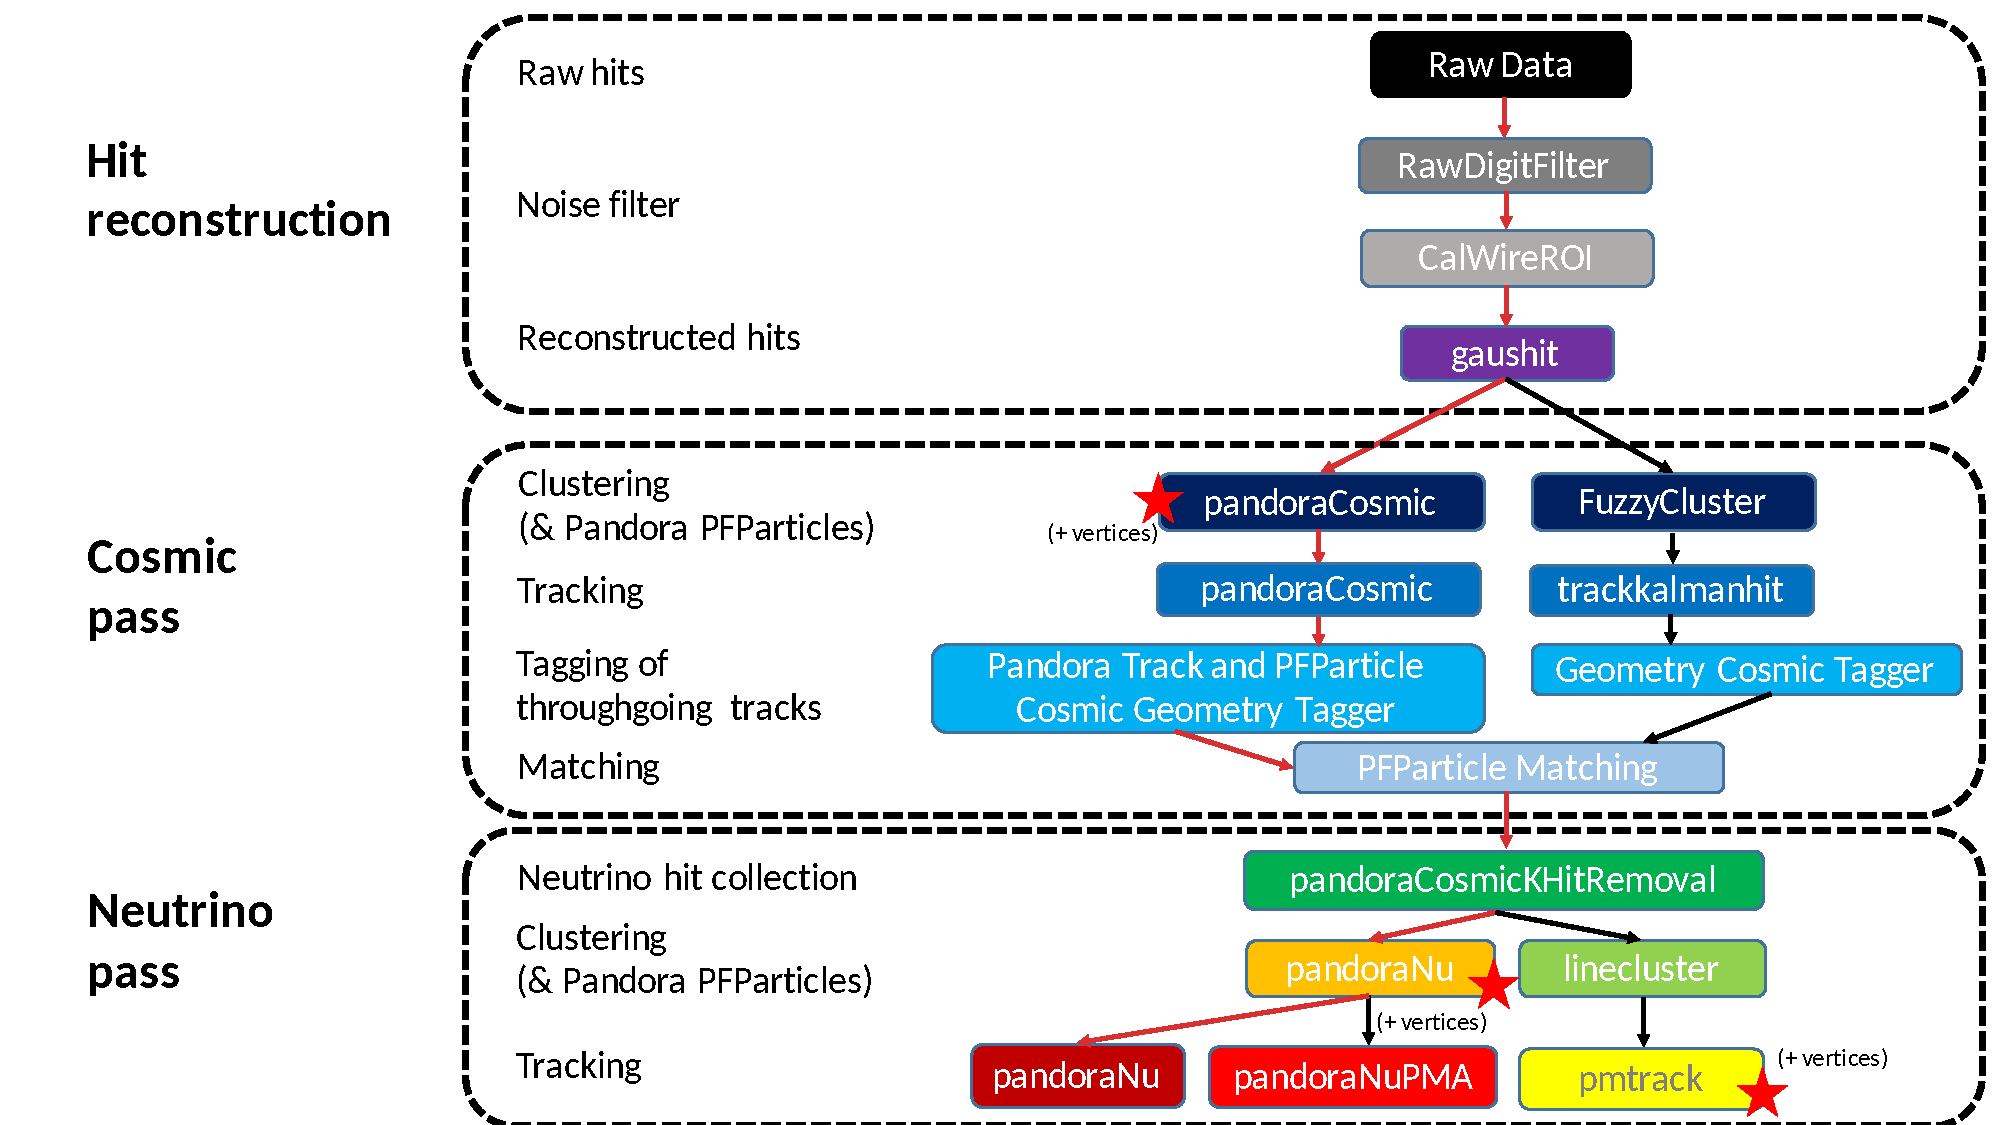
\includegraphics[width=1.0\textwidth]{images/FirstCCInclusive/RecoChart.pdf}
    \caption[Reconstruction Chain of \textbf{uboonecode} v05.08.00]{Depicted above are the full reconstruction chains available with \textbf{uboonecode} v05.08.00, featured in \cite{MicroBooNECCInclPN}. The red arrows indicate the reconstruction chain used in my analysis. The red stars on some of the boxes indicate that the algorithms return reconstructed \gls{3d} \glspl{Vertex}.}
    \label{fig:RecoChain}
\end{figure}

The charge readout wire signal waveforms (see section \ref{sec:ChargeReadout} and figure \ref{fig:WireSignals}) first passes a software noise filter tuned to each wire's specific noise levels and frequencies \cite{MicroBooNENoiseFilterPN}. As the input waveforms represent the largest single volume of data in a MicroBooNE event, this filter is also used to reduce the length of the waveforms from their input \num{9600} time samples (also called ticks) to \num{6400} time samples. After noise filtering the waveforms are passed to the deconvolution algorithm which aims to remove the effects of the charge carrier drift and electronics response in order to get a measurement of the number of \glspl{quasifreeelectron} created by the incident particles. At the same time, potential \gls{roi} in the waveforms are identified by using simple signal thresholds. These \gls{roi} then pass through a hit finding algorithm which identifies the peaks in the waveforms and attempts to fit them with a Gaussian distribution. If the fit quality is deemed sufficient, a hit is identified and its peak time and width is stored. In conclusion, a hit is a data product of a charge signal recorded on a single wire at a certain time and thus, features two dimensions given by the wire position and \gls{quasifreeelectron} drift, as shown in section \ref{sec:ChargeDrift}. 

In the next step, hits expected to be correlated in space and time are grouped into so-called \glspl{Cluster}. This clustering is done separately for each charge readout plane and the resulting \glspl{Cluster} create three \gls{2d} images. Thereafter, these \gls{2d} images are combined to reconstruct a \gls{3d} object. This is achieved with elaborate pattern recognition algorithms which use the common drift coordinates of the clustered hits from different planes. In the \gls{Pandora} framework the resulting \gls{3d} objects are called \textbf{PFParticles}. They are characterised either as track-like or shower-like according to the pattern of their \gls{2d} hits. These associated hits are also stored in the data and linked to by the PFParticle. This allows for multiple passes of different algorithms. Every PFParticle features a \gls{Vertex} position at the point of its first energy deposition. Moreover, the topological association between PFParticles are also used to identify parent-daughter relationships. These relationships are then collated into a particle hierarchy. In this way every particle can be associated to a primary \gls{Vertex}, \ie the primary particle interaction point \cite{PandoraLAr}. 

The \gls{3d} reconstruction process is staged in two different passes, employing different algorithms. The first is called \textbf{cosmic pass} or \textbf{pandoraCosmic}, whereby the applied algorithms are optimised for cosmic-ray muon reconstruction. This means, the algorithms are more track-oriented. Shower-like PFParticles are assumed to be correlated to delta rays and are hence declared as daughter particles by default. Furthermore, the primary \gls{Vertex} of every track-like PFParticles is positioned at the end point of the track with the highest $y$-coordinate value (see the detector coordinate system in figure \ref{fig:MicroBooNECoordinateSystem}). In this cosmic pass, tracks are flagged as unambiguous cosmic-rays if:
\begin{enumerate}
    \item some of the associated hits are apparently placed outside of the \gls{tpc} at the trigger time $t_0$, \ie they seem to be cosmic background pileup events (see section \ref{sec:CosmicPileup});
    \item the reconstructed trajectories are through-going, \ie their start and end points are both located at two \gls{tpc} boundaries.
\end{enumerate}
In the latter condition, tracks going through the upstream and downstream end simultaneously are an exception and not flagged unambiguous cosmic-rays, since they could be related neutrino events with a \gls{Vertex} outside of the active volume, so-called \textbf{dirt events}. All PFParticles with their associated hits, which are not flagged as unambiguous cosmic, are then subject to a second pass. This second reconstruction stage is called \textbf{neutrino pass} or \textbf{pandoraNu}. As the name implies, the reconstruction algorithms employed are optimised for neutrino interactions. They also ensure that each PFParticle emerging from a \gls{Vertex} is reconstructed as individuals. Finally, \gls{Pandora} adds a parent neutrino particle to the hierarchy \cite{MicroBooNECCInclPN,PandoraLAr}. Note, that both reconstruction passes also provide $\langle -dE/dx \rangle$ information, although this feature was not used in this analysis. In the upcoming selection process, only pandoraNu reconstructed data was used. In the case of \gls{mc} samples, it is vital to have access to the truth information of reconstructed tracks and showers. For this purpose, \gls{LArSoft} keeps track of a particle's true properties from simulation through reconstruction. This so-called \textbf{back tracker} is vital for background estimates, evaluating detector effects, and determining efficiencies.

As will be shown later in section \ref{sec:EventSelection}, my event selection requires muon track containment in order to reliably calculate muon momentum. The containment allows for the use of $\langle -dE/dx \rangle$ for track momentum reconstruction, see section \ref{sec:EnergyDissipationCharged}. For my analysis, I used an integrated form of $\langle -dE/dx \rangle$ (see equation \ref{eq:BetheBloch}). More precisely, the muon momentum for various total track lengths was determined by numerical integration. These data points were then interpolated by a 3\textsuperscript{rd} degree \gls{Spline} in order to provide a continuous conversion function shown figure \ref{fig:MomentumSpline}.
\begin{figure}[htbp]
    \centering
    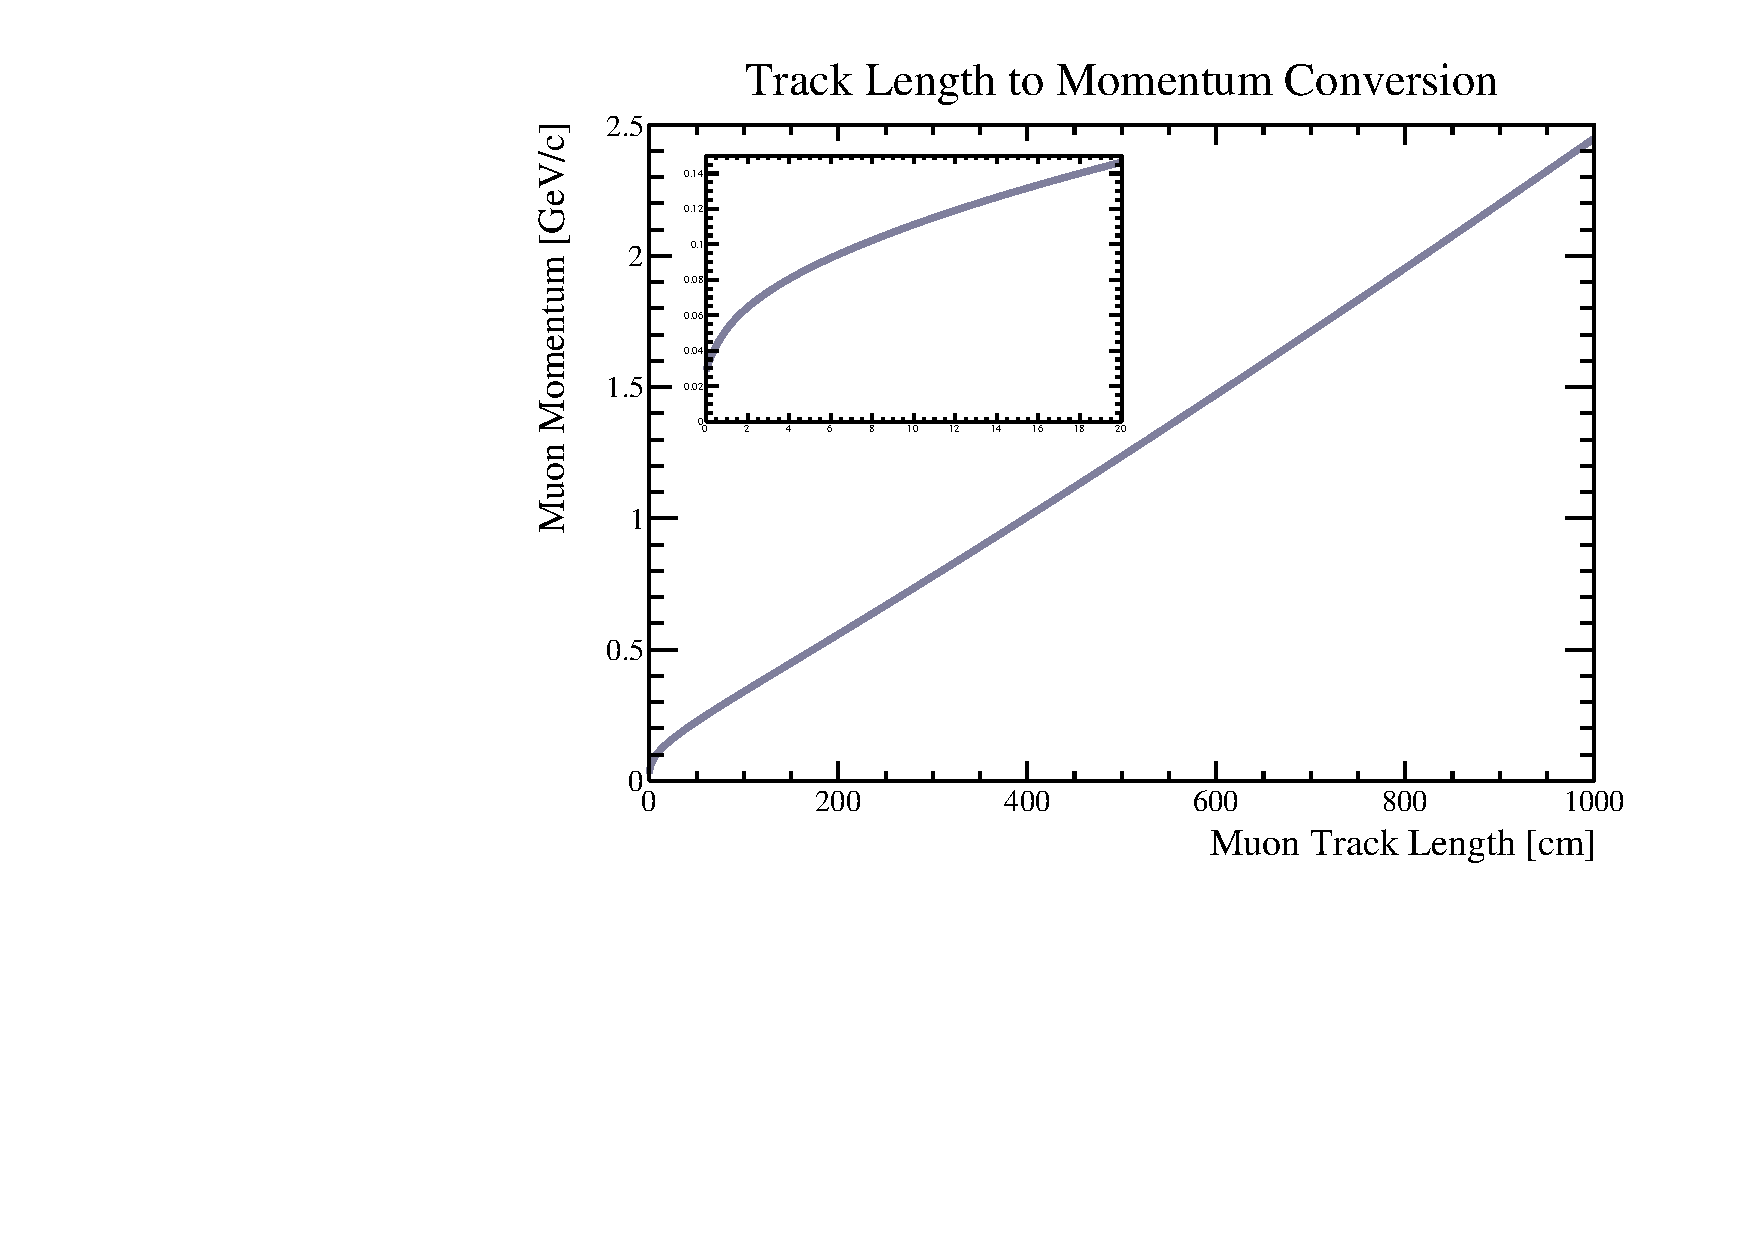
\includegraphics[width=1.0\textwidth]{images/FirstCCInclusive/TrackLengthMomentumRelation.pdf}
    \caption[Track Length to Momentum Conversion Function]{This graph shows the function (\gls{Spline}) for a track length to momentum conversion for a muon. The relation is almost linear for higher energies due to the \gls{mip} properties of the muon. A closeup graph in the upper left corner shows the steep drop at short track lengths which is related to the \textbf{Bragg peak}.}
    \label{fig:MomentumSpline}
\end{figure}
In the analysis, I simply evaluated the \gls{Spline} at the reconstructed track length and filled the momentum histograms with the result. 

\section{Event Selection} \label{sec:EventSelection}
An event selection aims to select as many signal events as possible, while avoiding as many background events as possible. These are mostly contradicting goals and therefore, keeping these analysis aims in mind, while developing the selection, is of great importance. For selecting $\nu_{\mu}$ we are first looking for a scintillation \gls{Flash} coinciding with the \gls{BeamGate}. The charge signal must feature at least one \gls{Vertex} with a single muon track, carrying most of the energy of the interaction. This means we are looking for a long \gls{mip} track within the \gls{tpc} in coincidence with a \gls{Flash}.

The \gls{cc} inclusive neutrino event selection method used in this analysis is based on a previous \gls{mc} performance study \cite{MCPerfPublicNote}. I further developed and refined said selection into an nine step process as summarised in the list below:
\begin{enumerate}
    \item At least one \gls{Flash} of $>$ \num{50} \gls{pe} within the \gls{BeamGate}.
    \item The beam gate \gls{Flash} with the highest \gls{pe} count is selected as \gls{Flash} candidate.
    \item At least one track originating within \SI{5}{\centi \metre} around a \gls{Vertex}.
    \item The \gls{Vertex} with the most forward going tracks is selected as the \gls{Vertex} candidate.
    \item The \gls{Vertex} candidate is located in the \gls{fv}.
    \item The longest track associated with the \gls{Vertex} is selected as muon track candidate.
    \item The track candidate is within \SI{80}{\centi \metre} of the \gls{Flash} ($z$-axis only).
    \item The track candidate is fully contained.
    \item The track candidate's range is greater than \SI{75}{\centi \metre}.
\end{enumerate}
Above sequence is described in more detail in the next paragraph. In general, my selection aims at identifying the muon from a \gls{cc} muon neutrino interaction and does not bias towards track multiplicity. However, in order to sufficiently reduce the cosmic background, the analysis is strongly biased towards forward-going tracks. At the time this selection was performed, the software tools to determine the muon momentum by multiple Coulomb scattering (see section \ref{sec:EnergyDissipationCharged}) were not yet advanced enough to be used. Hence, the selection requires muon track containment in the \gls{tpc}'s \gls{fv} for muon energy reconstruction purposes. All this limits the phase space and reduces the acceptance. The selection sequence itself can be divided into three parts: first, the scintillation \gls{Flash} candidate selection, second, the \gls{Vertex} candidate selection, and finally, the muon track candidate selection.
% TODO cut optimisation

The first step in my selection sequence is a cut requiring at least one light readout system \gls{Flash} in the event's \gls{BeamGate} with more than \num{50} \glspl{pe} on all \gls{pmt} photocathodes combined, see section \ref{sec:MicroBooNELightDetection}. If there are multiple \glspl{Flash}, the strongest is selected as \gls{Flash} candidate, \ie the one with the highest total \gls{pe} count. This already concludes the \gls{Flash} selection part of the sequence.

Then, all reconstructed \glspl{Vertex} featuring at least one track, originating within a distance \SI{5}{\centi\metre}, are selected. All reconstructed information of said \glspl{Vertex} and their associated tracks are then stored for further selections. For the next step, the \gls{Vertex} with the most forward directed tracks has to be determined. The forwardness of a track is measured by the product of the track range $R$ times the cosine of the incident angel $\theta$. The former is defined as the distance between the track's start and end points. As a reference for the latter, consider MicroBooNE's coordinate system shown in figure \ref{fig:MicroBooNECoordinateSystem}. The sum of all these products of every \gls{Vertex} associated track divided by the sum of their combined track range then gives the forwardness, $f$, \ie
\begin{equation} \label{eq:Forwardness}
    f = \frac{\sum_{i=0}^{N} R_i \cos\left( \theta_i \right)}{\sum_{i=0}^{N} R_i},
\end{equation}
with $N$ denoting the total number of tracks associated to the \gls{Vertex}. In other words, the forwardness is simply a weighted average of $\cos{(\theta)}$. Since the reconstruction of track directionality could not be trusted at that time, I actually used the absolute value of the forwardness, $|f|$. Thereafter, the \gls{Vertex} exhibiting the largest value of $|f|$ is selected as the primary neutrino \gls{Vertex} candidate and all other \glspl{Vertex} are discarded. Up to this point, the selection strategy was to find the most likely neutrino interaction candidate, before applying geometrical cuts. This procedure reduces the chance of the misidentification of cosmic events as \gls{bnb} related events and marks the main difference to the original scheme \cite{MCPerfPublicNote}. After the \gls{Vertex} candidate is selected, a \gls{fv} cut is applied. In this analysis the cut is set at \SI{20}{\centi\metre} from the top and bottom of the active volume on the $y$-axis and \SI{10}{\centi\metre} from every other side ($x$ and $z$ axis) of the active volume. This cut concludes the \gls{Vertex} selection process. 

From this point forward, only the tracks associated with the \gls{Vertex} candidate are considered. First, the track with the greatest track range is tagged as the muon track candidate. Next, said track candidate is matched to the before selected \gls{Flash} candidate employing a rudimentary \gls{1d} matching method. For this, the $z$-coordinate of the reconstructed \gls{Flash} centre is used as the point of reference. Now, only if the closest track point is within \SI{80}{\centi\metre} distance in $z$ from the \gls{Flash} centre, the track will pass the selection. As discussed in section \ref{sec:CosmicPileup}, the use of a \gls{Flash} matching process is rooted in the desire to remove cosmic pileup tracks from the selection. Thereafter, track containment of the candidate is required for muon momentum reconstruction purposes. Finally, as a last cut, a candidate track range of at least \SI{75}{\centi\metre} is required. This step was found optimal to reduce \gls{nc} events as well as additional cosmic background. Interestingly, it also cuts the drop-off in neutrino flux at energies below $\sim \SI{300}{\mega\electronvolt}$. The maximum neutrino energy is limited by the containment requirement to $\sim \SI{2.5}{\giga\electronvolt}$. Events surviving all nine selection steps, are considered to be muon neutrino \gls{cc} interactions.

Some of the cut values used in this selection were optimised for the maximum product of purity times efficiency (definition is in section \ref{sec:SelectionYields}). This is equivalent to finding the maximum of the metric $S/\sqrt{S+B}$, where $S$ denotes the number of signal events and $B$ the number of background events \cite{ProgressInNuMeasurements}. Naturally, the metric is calculated with \gls{mc} samples, since truth information is paramount for the background and signal determination. Then a variable cut value is applied to these \gls{mc} samples. In this process the values $S$ and $B$ are determined for every cut value and the metric $S/\sqrt{S+B}$ filled into a histogram. Two examples of these cut optimisation histograms are shown in figure \ref{fig:CutOptimisations}.
\begin{figure}[htbp]
    \centering
    \subfloat[][]
    {
        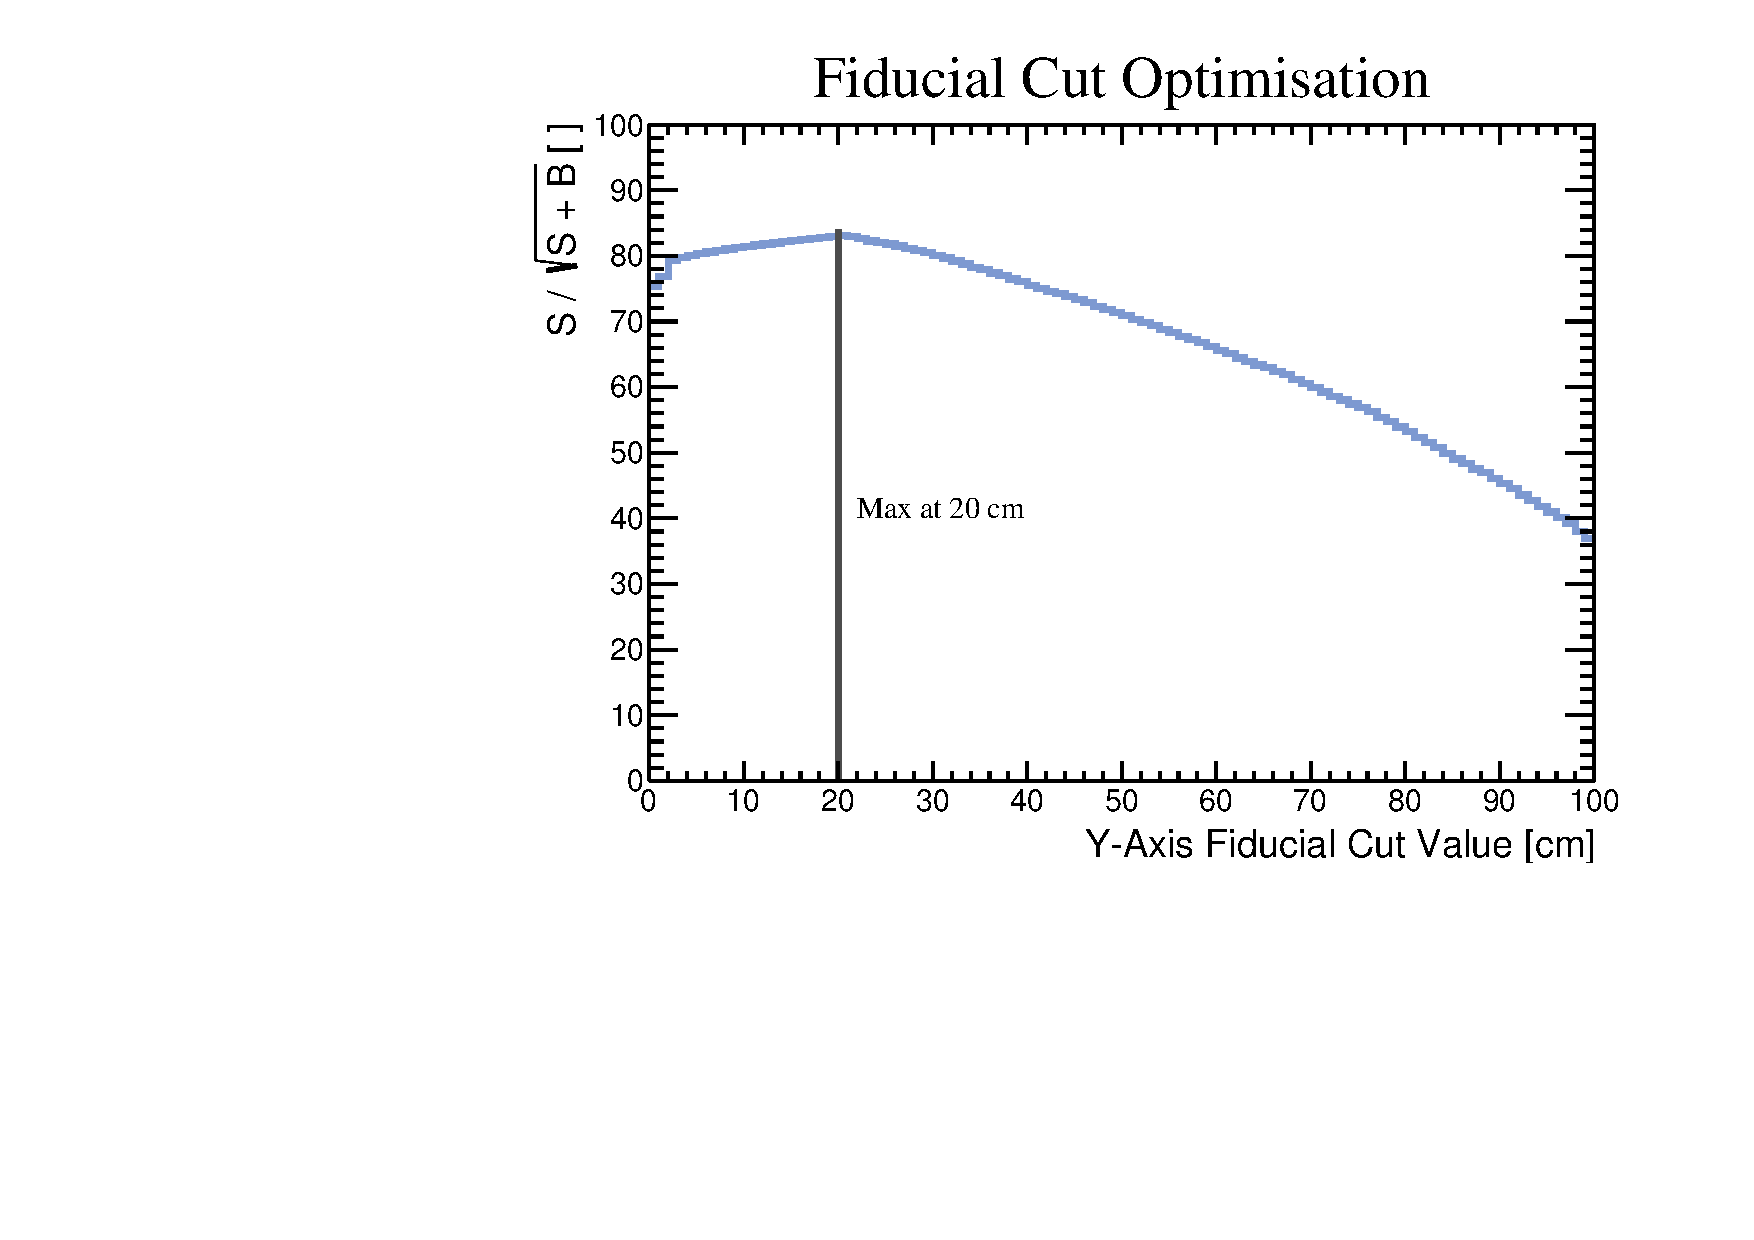
\includegraphics[width=0.5\textwidth]{images/FirstCCInclusive/CutOptFiducialY.pdf}
        \label{fig:CutOptFiducialY}
    }
    \subfloat[][]
    {
        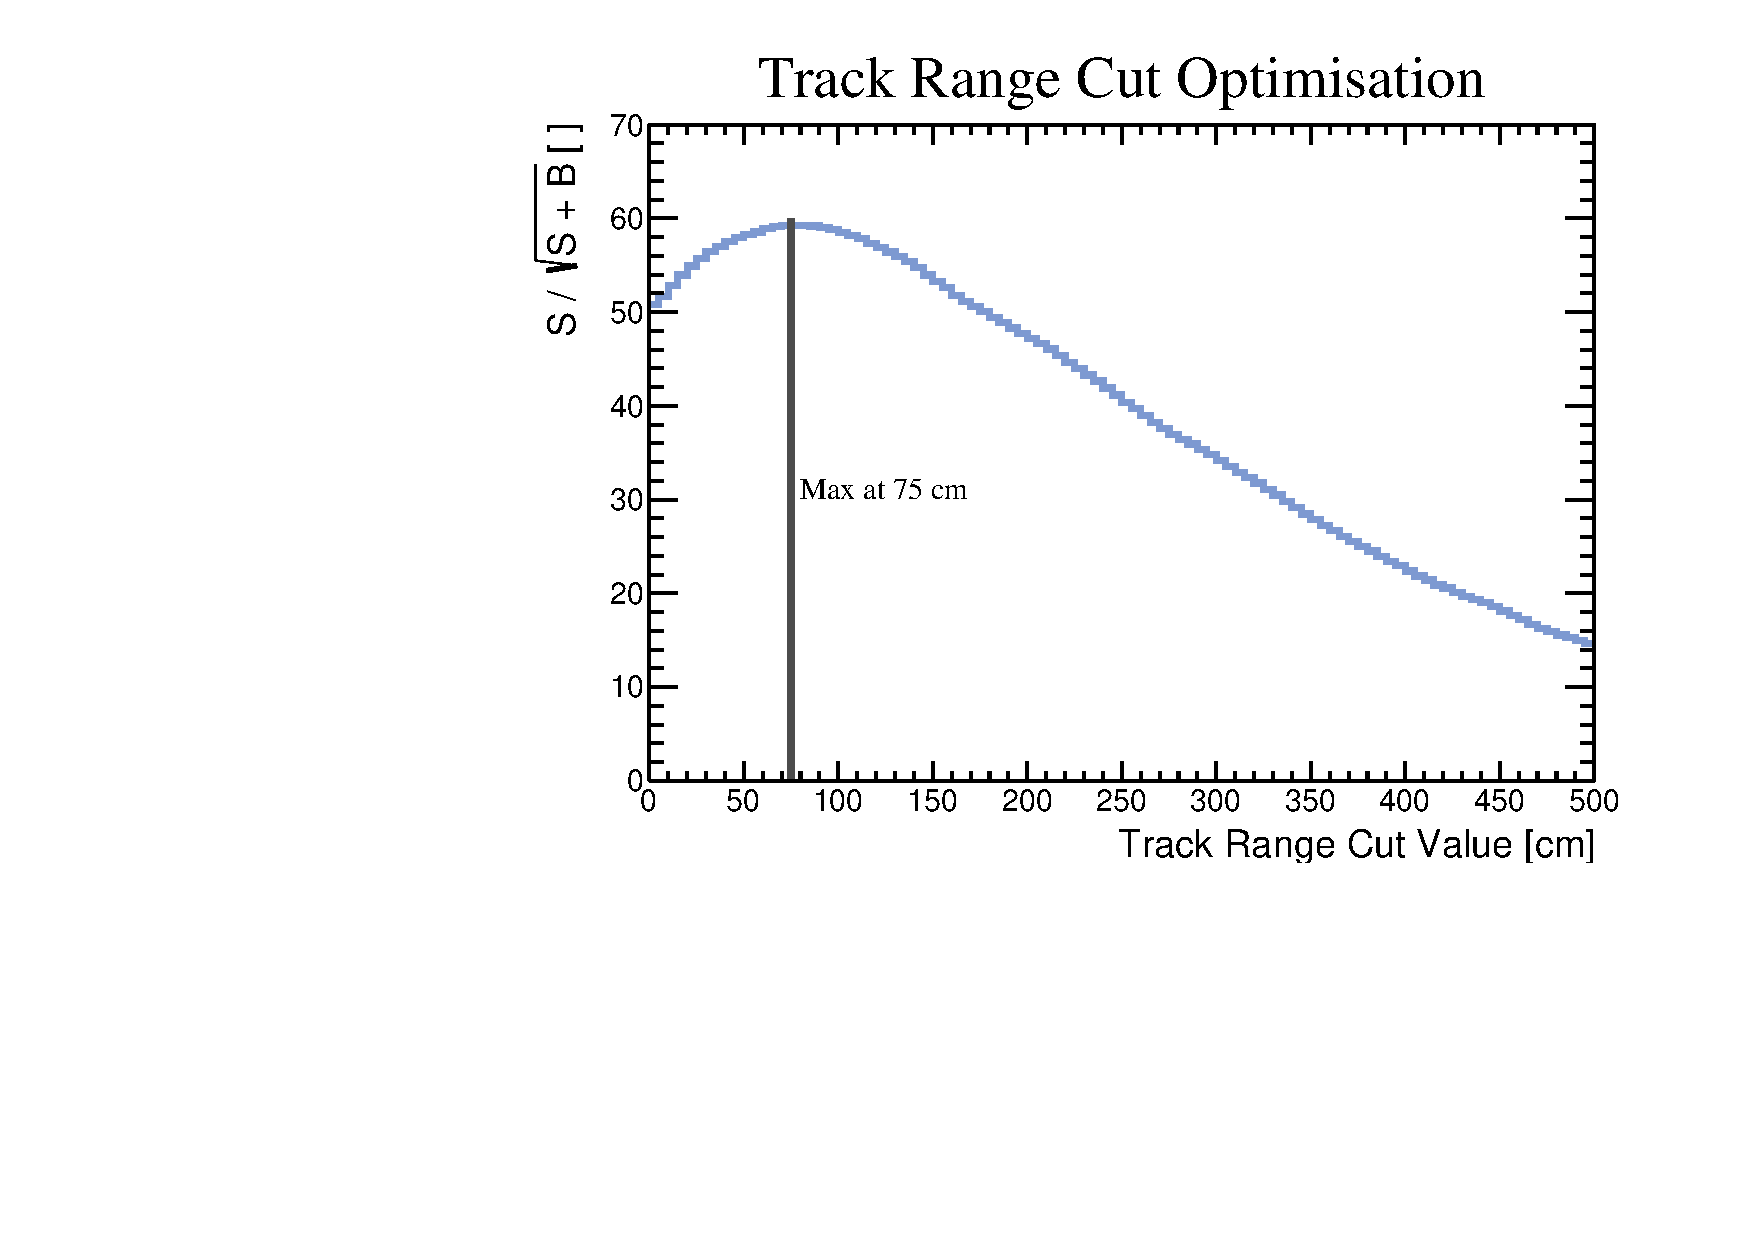
\includegraphics[width=0.5\textwidth]{images/FirstCCInclusive/CutOptTrackRange.pdf}
        \label{fig:CutOptTrackRange}
    }
    \caption[Cut Optimisation Graphs]{Above are two examples of the track optimisation performed for this analysis. \subref{fig:CutOptFiducialY} shows the metric $S/\sqrt{S+B}$ as a function of the $y$-axis fiducial cut value. \subref{fig:CutOptTrackRange} shows the same metric, but as a function of the minimal track range cut value.}
    \label{fig:CutOptimisations}
\end{figure}
However, the use of this metric is only allowed when the systematic uncertainty on the background can be neglected \cite{ProgressInNuMeasurements}. As I will show later, there were still many uncertainties concerning MicroBooNE's simulation and reconstruction tools at the time this analysis was performed. Hence, above-described procedure was only used for the \gls{fv} cut in all three axis, the track to \gls{Flash} distance cut, and the track range cut. The optimal \gls{Flash} intensity cut value of \num{50} \gls{pe}, for instance, was determined by direct measurements \cite{MicroBooNEFirstNuPN}. In contrast, the \gls{mc} samples suggest a value of \num{190} \gls{pe}, hinting at discrepancies between the \gls{Flash} simulation models and real \glspl{Flash}. Lastly, the metric of the track-to-\gls{Vertex} distance cut shows a maximum at \SI{0}{\centi\metre}. In order to account for slight discrepancies between \gls{mc} and \gls{tpc} data reconstruction, I set this cut value to \SI{5}{\centi\metre}. However, this selection step has very little influence on the number of selected events, as will be shown in tables \ref{tab:PassingRatesData} and \ref{tab:PassingRatesMC}.

\section{Event Rate and Cross Section Results} \label{sec:CrossSectionResults}
A result of this analysis was presented as part of a MicroBooNE public note with the title: ``Selection and kinematic properties of $\nu_\mu$ \gls{cc} inclusive events in \num{5e19} \gls{pot} of MicroBooNE data'' \cite{MicroBooNECCInclPN}. For this note we presented forward-folded kinematic distributions of $N^\text{Sel}_\nu$, \ie selected on-beam subtracted by the properly scaled selected off-beam data, see equation \ref{eq:NumberOfNu}. Back then, I was asked to normalise the data and \gls{mc} distributions by on-beam distributions' integral and not by their \gls{pot}. For this thesis, however, I would like to present \gls{pot} normalised numbers. Moreover, in view of the most recent results, I chose to present the kinematic distributions in a fully forward-folded form, where all backgrounds are added to the \gls{mc} sample. This includes the reducible cosmic background of the off-beam data set. This method allows for the comparison of the \gls{mc} models to the undeterred on-beam data, and hence, follows the true spirit of forward-folding. This leads to differential yield distributions as a function of the kinematic properties of the selected tracks and vertices which will be shown in section \ref{sec:KinematicDistributions}.

\subsection{Selection Rates and Yields} \label{sec:SelectionYields}
The influence of the various selection steps on both data samples (see section \ref{sec:MCSamples}) are shown in \ref{tab:PassingRatesData}, while the same is shown for the \gls{mc} \gls{bnb} Baseline sample (see section \ref{sec:MCSamples}) in table \ref{tab:PassingRatesMC}.
\begin{table}[htbp]
    \centering
    \caption[Selection Passing Yields for Data Samples]{This table shows passing yield for the previously described event selection, applied to on-beam and off-beam data. The numbers in brackets give the passing rate with respect to the step before (first percentage) and with respect to the generated events (second percentage). Note that the off-beam data stream is additionally presented as scaled by factor $N_\text{Gate}^\text{BNB} / N_\text{Gate}^\text{EXT} = \num{1.23}$ to normalise it to the on-beam data stream.}
    \begin{tabu}{lrl|rrl}
        \toprule
        \rowfont[c]{\bf} Selection Step & \multicolumn{2}{c|}{on-beam} & \multicolumn{3}{c}{off-beam} \\
        & & & Measured & Scaled & \\
        \midrule
        Triggered & 546910 & & 388471 & 477819 & \\
        $\ge$ 1 flash $\ge$ \num{50} \gls{pe} & 135923 & (25\%$\mid$25\%) & 78657 & 96748 & (20\%$\mid$20\%)\\
        $\ge$ 1 track - Vtx $\le$ \SI{5}{\centi \metre} & 134744 & (99\%$\mid$25\%) & 77868 & 95778 & (99\%$\mid$20\%)\\
        Vertex in \gls{fv} & 74827 & (55\%$\mid$14\%) & 41844 & 51468 & (54\%$\mid$11\%) \\
        Flash matching track & 22059 & (29\%$\mid$4.0\%) & 9946 & 12234 & (24\%$\mid$2.6\%)\\
        Track containment & 10722 & (49\%$\mid$1.9\%) & 4295 & 5283 & (43\%$\mid$1.1\%)\\
        Track range $\ge$ \SI{75}{\centi \metre} & 3213 & (30\%$\mid$0.6\%) & 1080 & 1328 & (25\%$\mid$0.3\%)\\
        \bottomrule
        \label{tab:PassingRatesData}
    \end{tabu}
\end{table}
\begin{table}[htbp]
    \centering
    \caption[Selection Passing Yields for the Baseline MC Sample]{The table below shows passing yield of the above-described event selection, applied to the \gls{mc} \gls{bnb} Baseline sample in the left column. This contains all events, not just $\nu_{\mu}$ \gls{cc} inclusive. In the right column, the yield of true $\nu_{\mu}$ \gls{cc} inclusive events are shown, including events outside of the \gls{fv}. Both yields correspond to \num{2.30e20} \gls{pot}. The numbers in brackets again give the passing rate with respect to the step before (first percentage) and with respect to the generated events (second percentage).}
    \begin{tabu}{lrl|rl}
        \toprule
        \rowfont[c]{\bf} Selection Step & \multicolumn{4}{c}{BNB Baseline} \\
        & \multicolumn{2}{c|}{Selection} & \multicolumn{2}{c}{True $\nu_\mu$ \gls{cc}} \\
        \midrule
        Generated events & 191362 & & 46820 &  \\
        $\ge$ 1 flash $\ge$ \SI{50}{PE} & 136219 & (71\%$\mid$71\%) & 44002 & (94\%$\mid$94\%) \\
        $\ge$ 1 track - Vtx $\le$ \SI{5}{\centi \metre} & 135830 & (99\%$\mid$71\%) & 43974 & (99\%$\mid$94\%)\\
        Vertex in \gls{fv} & 79112 & (58\%$\mid$41\%) & 34891 & (79\%$\mid$74\%) \\
        Flash matching track & 40267 & (51\%$\mid$21\%) & 25891 & (74\%$\mid$55\%) \\
        Track containment & 19391 & (48\%$\mid$10\%) & 11693 & (45\%$\mid$25\%) \\
        Track range $\ge$ \SI{75}{\centi \metre} & 6920 & (36\%$\mid$3.6\%) & 5780 & (50\%$\mid$13\%)\\
        \bottomrule
        \label{tab:PassingRatesMC}
    \end{tabu}
\end{table}
Considering the \gls{mc} selection results, it is striking that, the most effective step seems to be the cut of \glspl{Flash} below \num{50} \gls{pe}. It removes almost \SI{30}{\percent} of total number of event while only reducing the true $\nu_\mu$ \gls{cc} inclusive events by \SI{6}{\percent}. The track distance to \gls{Vertex} cut seems to exhibit quite a limited effect, as expected. Note, that it was introduced as a buffer, to mitigate expected differences in data and \gls{mc} \gls{Vertex} reconstruction. The \gls{fv} cut, also seems to reduce many background events with a event passing rate of \SI{58}{\percent} and a relatively low reduction of true signal events of \SI{21}{\percent}. Flash matching has a similar effect as the former step. Track containment removes almost the same percentage in total and true events alike. However, it is important to note, that this step was introduced for momentum reconstruction purposes and can thus not be circumvented. Lastly, the track range cut also boasts a relatively high efficacy with, \SI{36}{\percent} of total, and only \SI{50}{\percent} true reduction, respectively. Note, that the true $\nu_\mu$ \gls{cc} yields, listed in table \ref{tab:MCSamples}, contain events with true \gls{Vertex} positions outside of the \gls{fv}.

In order to calculate efficiency and purity of this selection, we have to define our signal first. For this, the signal event signature and the target properties have to be considered. The former is simple and already mentioned in the title of this very chapter, for we are only interested in $\nu_\mu$ \gls{cc} inclusive event signatures. For determining the target properties, however, the selection process itself is crucial. It has to be considered which steps change the target properties. The only cut this applies to, is the \gls{fv} cut. Therefore, we have our signal signature defined as: $\nu_\mu$ \gls{cc} inclusive events with a true \gls{Vertex} in the \gls{fv}. Hence, we also need to adapt the truth information of table \ref{tab:PassingRatesMC}. With this, we obtain \num{45266} generated signal events. When also requiring true \gls{Vertex} containment in \gls{fv} for the selected events, we get \num{5589} signal events. With both these numbers, we are able to calculate the overall efficiency, $\epsilon$, defined as 
\begin{equation}
    \epsilon \coloneqq \frac{\text{ Selected signal events }}{\text{ Generated signal events }} = \frac{\num{5589}}{\num{45266}} = \SI{12.3(14)}{\percent}.
\end{equation}

Furthermore, the truth information in the \gls{bnb} baseline \gls{mc} sample allows for the categorisation into selected signal and various background events. These categories are listed in table \ref{tab:SelectionBgrComposition}.
\begin{table}[htbp]
    \centering
    \caption[Selected Signal and Background Events of the Baseline MC Sample]{Listed in this table are the signal and background categories and their corresponding number of selected events. All events feature a true \gls{Vertex} inside of the \gls{fv} and the numbers remain unscaled, \ie they conform with \num{2.30e20} \gls{pot}. For this purpose, the off-beam data sample was scaled accordingly.}
    \begin{tabu}{llr}
        \toprule
        \rowfont[c]{\bf}Category & Description & Events \\
        \midrule
        Signal & $\nu_{\mu}$ \gls{cc} with true \gls{Vertex} in \gls{fv} & \num{5589} \\
        \midrule
        \multirow{7}{*}{Backgrounds}
        & Cosmic \gls{BeamGate} (off-beam) & \num{6172} \\
        & Cosmic pileup event & {688} \\
        & \gls{nc} events in \gls{fv} & \num{355} \\
        & Dirt events (out of \gls{tpc}) & \num{107} \\
        & Vertex out of \gls{fv} & {90} \\
        & $\bar \nu_{\mu}$ \gls{cc} events in \gls{fv} & \num{73} \\
        & $\nu_e$ and $\bar \nu_e$ \gls{cc} events in \gls{fv} & \num{18} \\
        \midrule
        & \textbf{Total backgrounds} & \num{7503} \\
        \bottomrule
        \label{tab:SelectionBgrComposition}
     \end{tabu}
\end{table}
In this table, the inclusion of the scaled number of selected off-beam events seems peculiar at first, but both, efficiency and purity, have to pertain to the selected on-beam events. As established in sections \ref{sec:DataSamples} and \ref{sec:MCSamples}, the direct compatibility of the on-beam and \gls{mc} samples are only given by either adding the off-beam to the \gls{mc} prediction or by subtracting it from the on-beam sample. The purity measures how many signal events are selected as a fraction of totally selected events and hence it is defined as,
\begin{equation}
    p \coloneqq \frac{\text{ Selected signal events }}{\text{Selected signal plus background events}} = \frac{\num{5589}}{\num{5589} + \num{7503} } = \SI{42.7(9)}{\percent}.
\end{equation}

\subsection{Kinematic Distributions} \label{sec:KinematicDistributions}
Figures \ref{fig:ForwardFoldedRangePhi} through \ref{fig:ForwardFoldedVertexPosition} show the distribution of kinematic quantities of the selected muon candidates. As mentioned before, these kinematic distributions are presented in forward-folded manner. This means that all backgrounds, including off-beam, are added to the \gls{mc} selection. Furthermore, all samples are scaled to \num{4.95e19} \gls{pot}. In this way, the combined \gls{mc} and background distributions become directly comparable to the unchanged on-beam selection distributions. To better exemplify the forward-folding method, the \gls{mc} plus background distributions, have their content broken down into \gls{mc} signal and various background categories, as introduced in table \ref{tab:SelectionBgrComposition}. The combined systematic and statistical uncertainties are added to the signal distribution as a partially transparent red band. The former will be discussed later in section \ref{sec:Systematics}. Every graph comes with its on-beam to \gls{mc} plus background ratio distribution. Moreover, all histograms feature \num{20} bins with constant bin size.

\begin{figure}[htbp]
    \centering
    \subfloat[][]
    {
        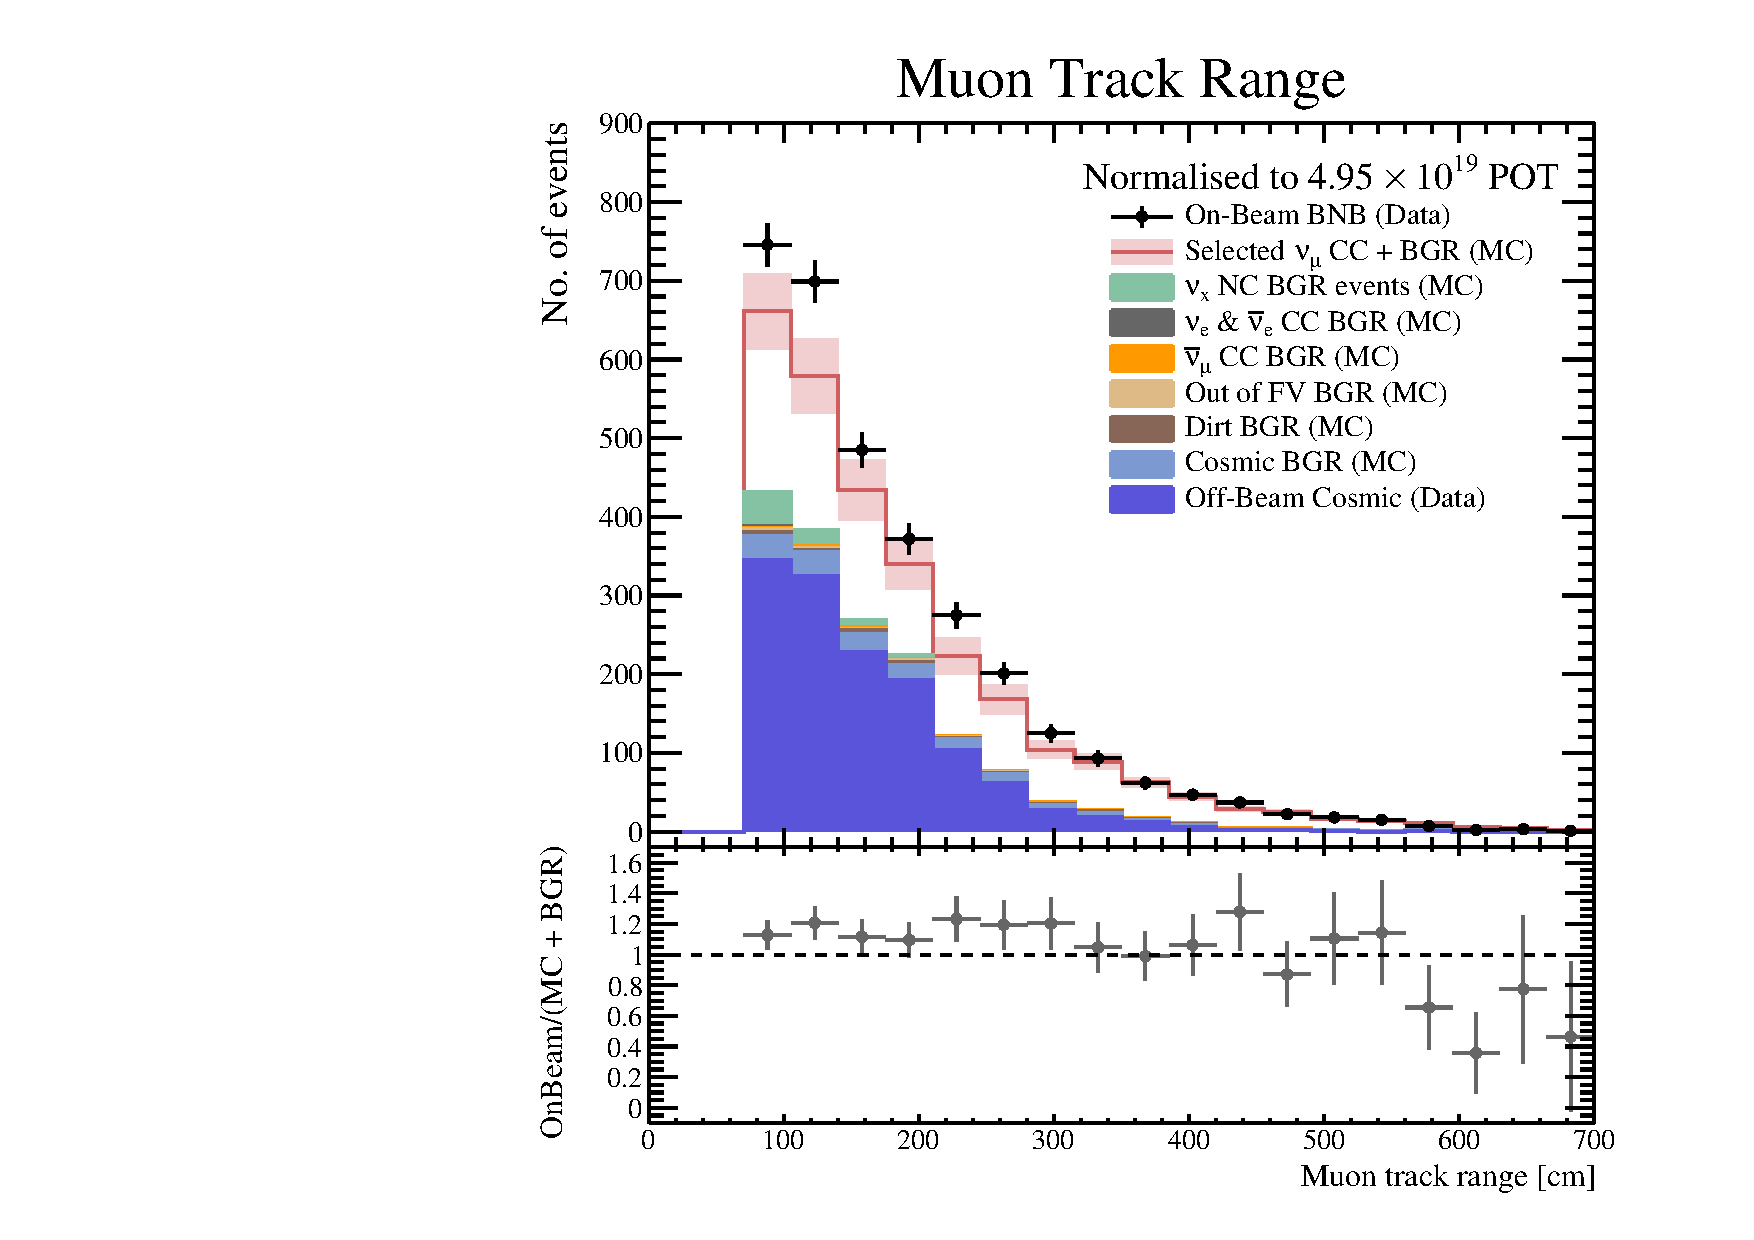
\includegraphics[width=0.5\textwidth]{images/FirstCCInclusive/Kinematic/ForwardFoldedTrackRange.pdf}
        \label{fig:ForwardFoldedTrackRange}
    }
    \subfloat[][]
    {
        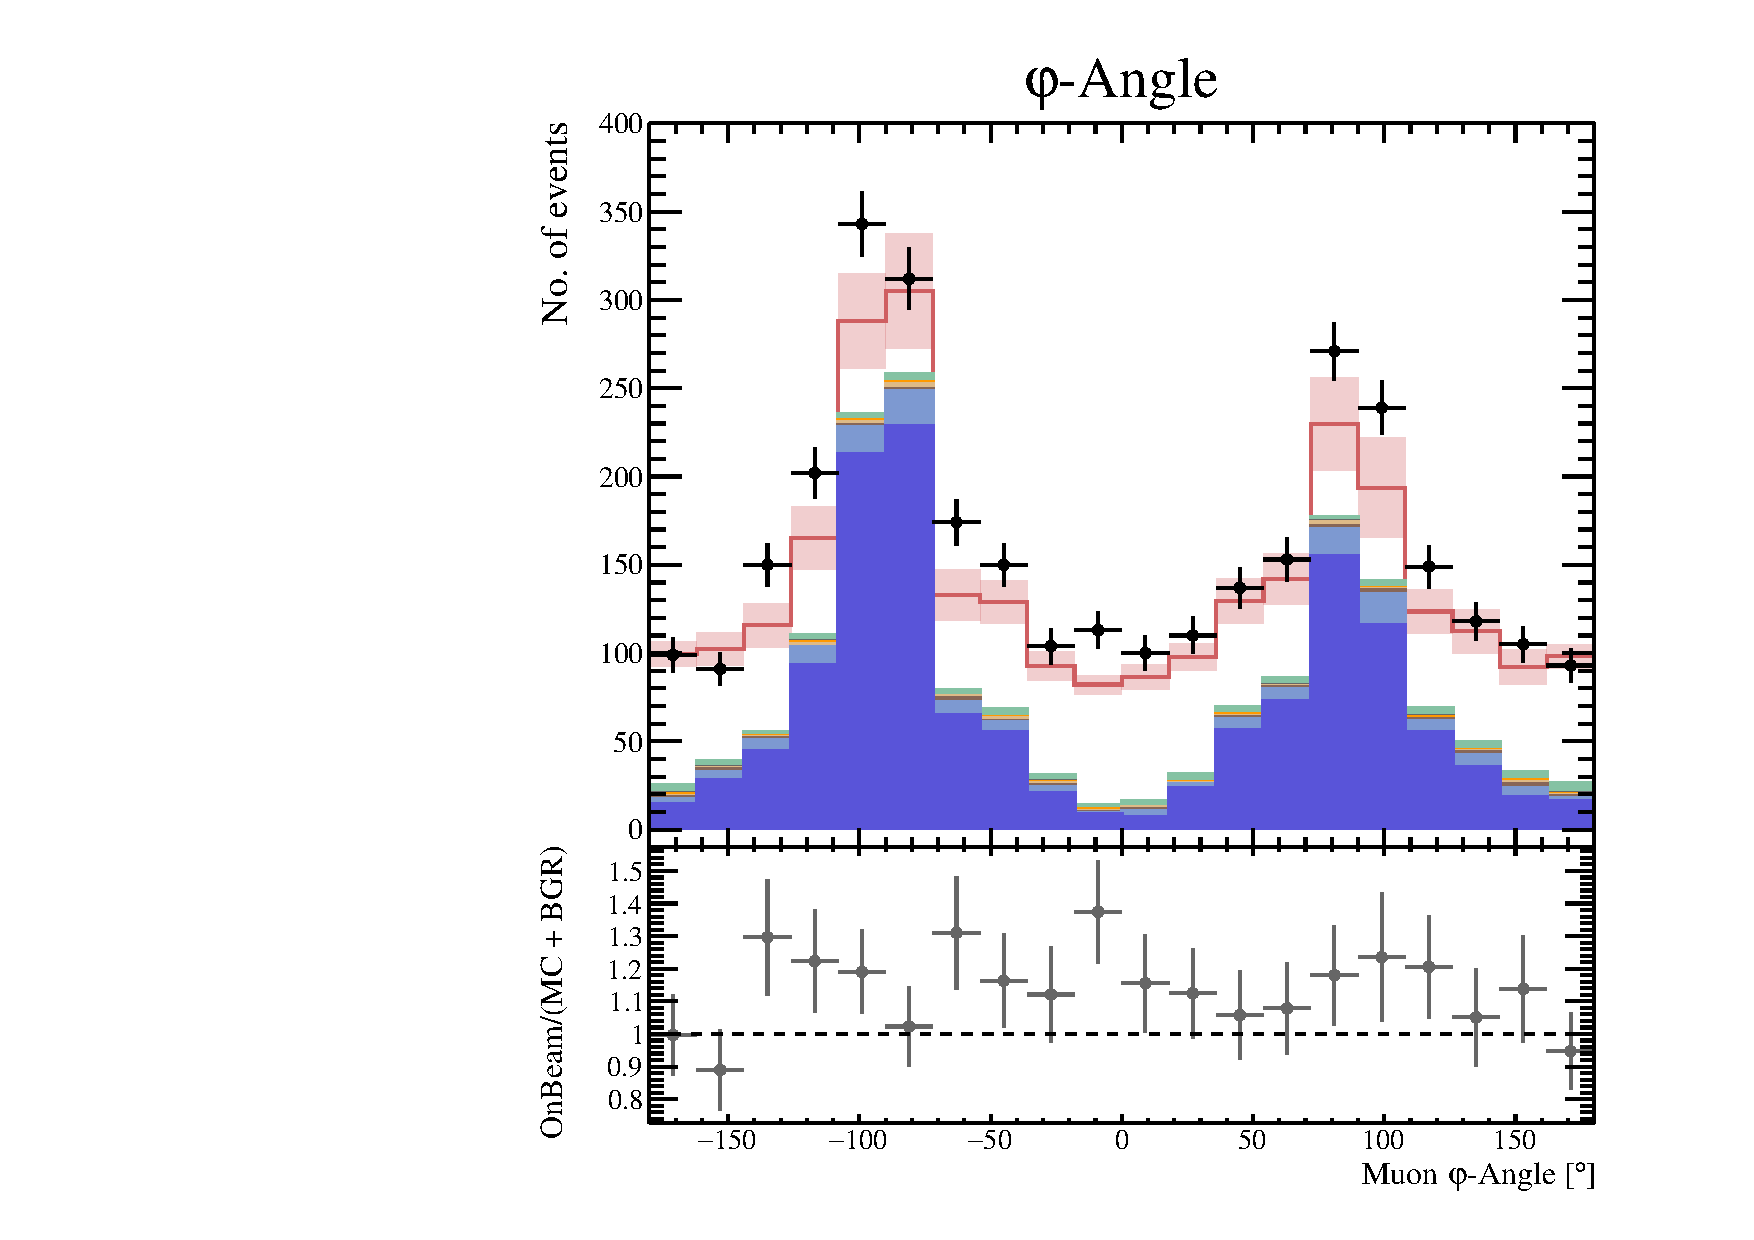
\includegraphics[width=0.5\textwidth]{images/FirstCCInclusive/Kinematic/ForwardFoldedPhi.pdf}
        \label{fig:ForwardFoldedPhi}
    }
    \caption[Forward-Folded Track Range and $\phi$-Angle Distributions]{Shown above are the forward-folded track range yield distribution \subref{fig:ForwardFoldedTrackRange}, and $\phi$-angle yield distributions \subref{fig:ForwardFoldedPhi}. The track range is depicted in the interval $[0,700] \si{\centi\metre}$ and $\phi$ in the range of $[-180,180] \si{\degree}$.}
    \label{fig:ForwardFoldedRangePhi}
\end{figure}
Figure \ref{fig:ForwardFoldedTrackRange} shows the forward-folded track range distribution. This is one of the graphs depicting a cut variable, wherefore there are no entries below \SI{75}{\centi\metre}. Interestingly, the dominant irreducible background for short track ranges seems to be caused by \gls{nc} neutrino interactions. This is expected, since \gls{nc} events usually do not feature any \glspl{mip}, but heavy hadrons with high stopping power. The on-beam to \gls{mc} plus background ratio shows a clear excess of on-beam events compared to the \gls{mc} prediction, especially in the high statistics bins. The forward-folded $\phi$-angle distribution in figure \ref{fig:ForwardFoldedPhi} also generally features an on-beam excess in almost all bins. Obviously, neutrino interactions should be isotropic in $\phi$, but cosmic interactions are not. Hence, the $\phi$ distribution is an interesting indicator for the cosmic background \gls{mc} model. Interestingly, there seems to be an excess of cosmic activity in the on-beam sample, indicated by the hump in the ratio graph around $\phi = \SI{90}{\degree}$, and to a minor extent slightly below \SI{-90}{\degree}. This cosmic feature is later discussed in section \ref{sec:Systematics}. Naturally, the shape of the forward-folded prediction is dominated by the two cosmic backgrounds at $\phi = \pm\SI{90}{\degree}$.

\begin{figure}[htbp]
    \centering
    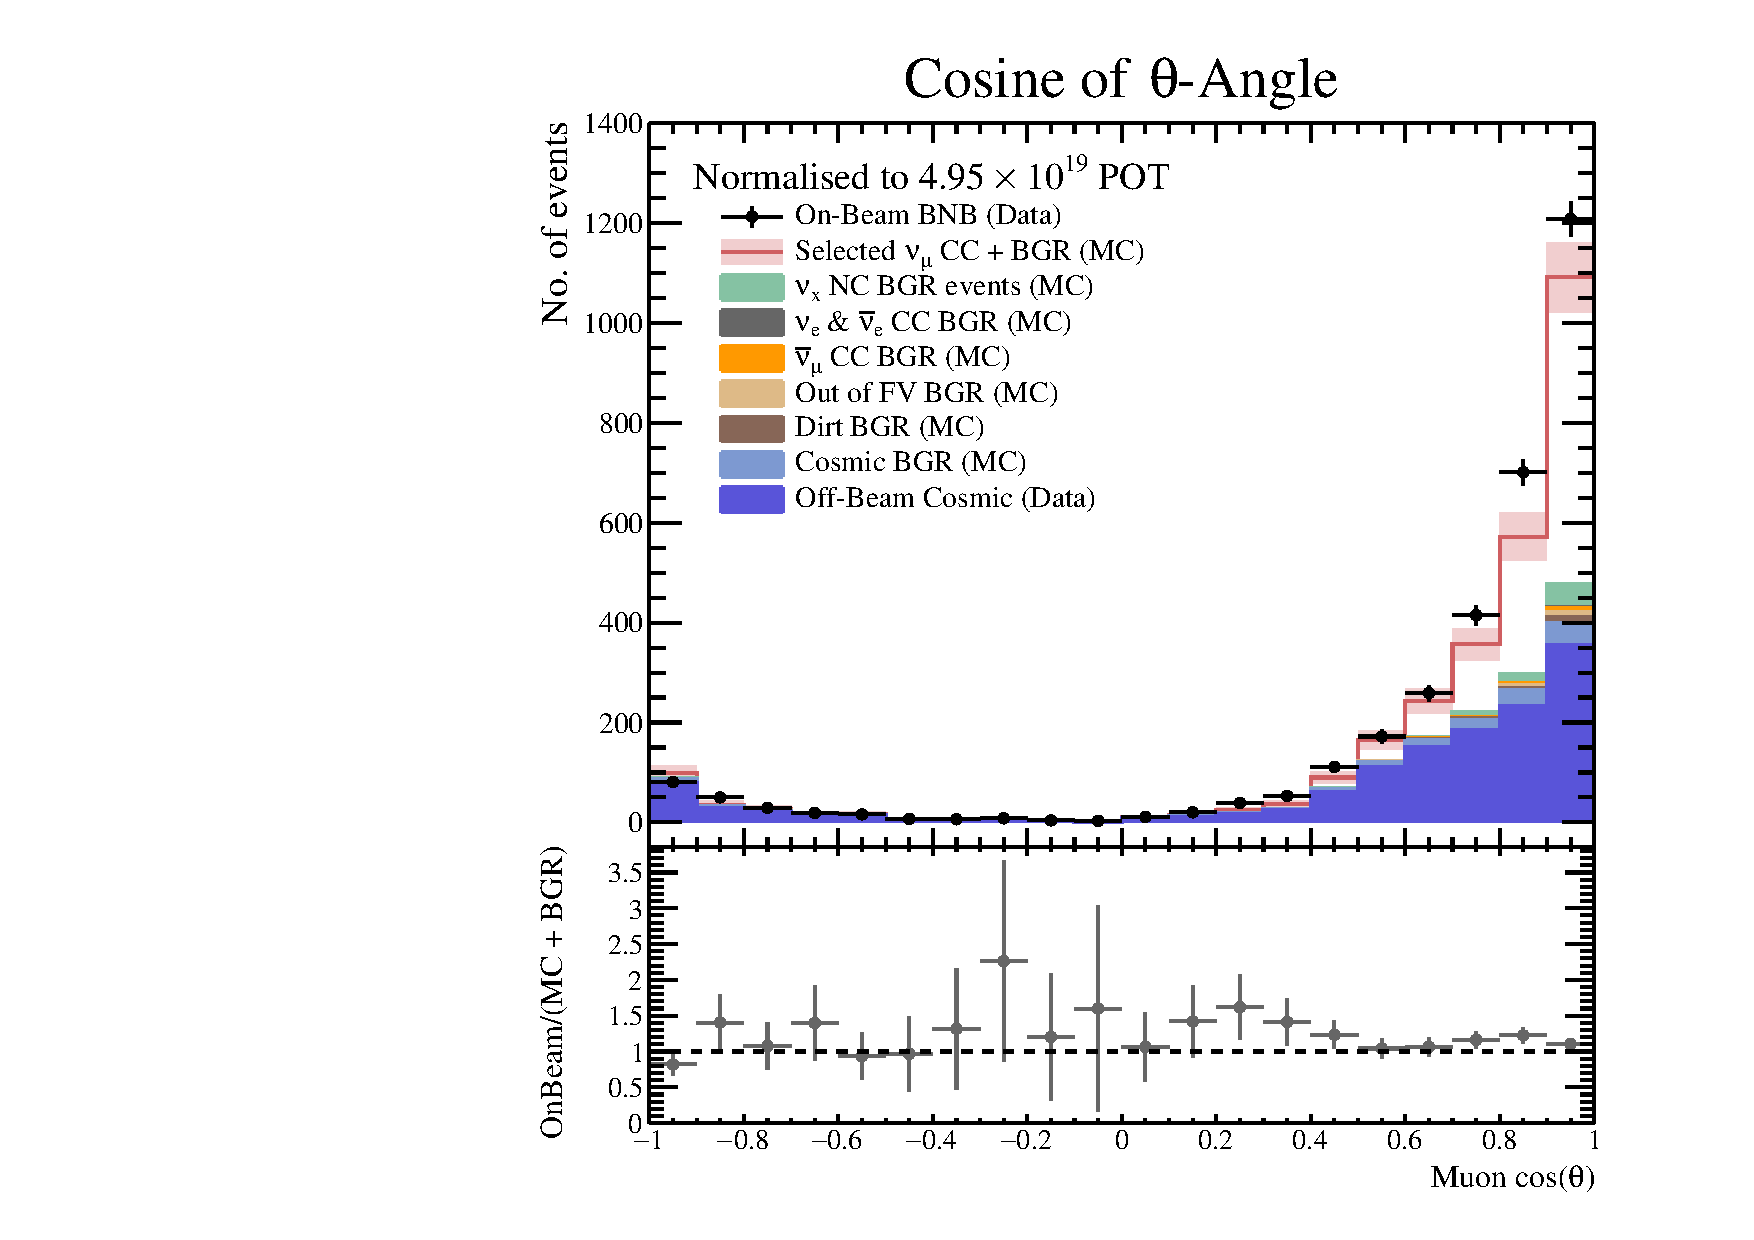
\includegraphics[width=0.8\textwidth]{images/FirstCCInclusive/Kinematic/ForwardFoldedCosTheta.pdf}
    \caption[Forward-Folded $\cos{(\theta)}$ Distribution]{Depicted here, is the forward-folded $\cos{(\theta)}$ yield distribution in the full interval $[-1,1]$.}
    \label{fig:ForwardFoldedCosTheta}
\end{figure}
\begin{figure}[htbp]
    \centering
    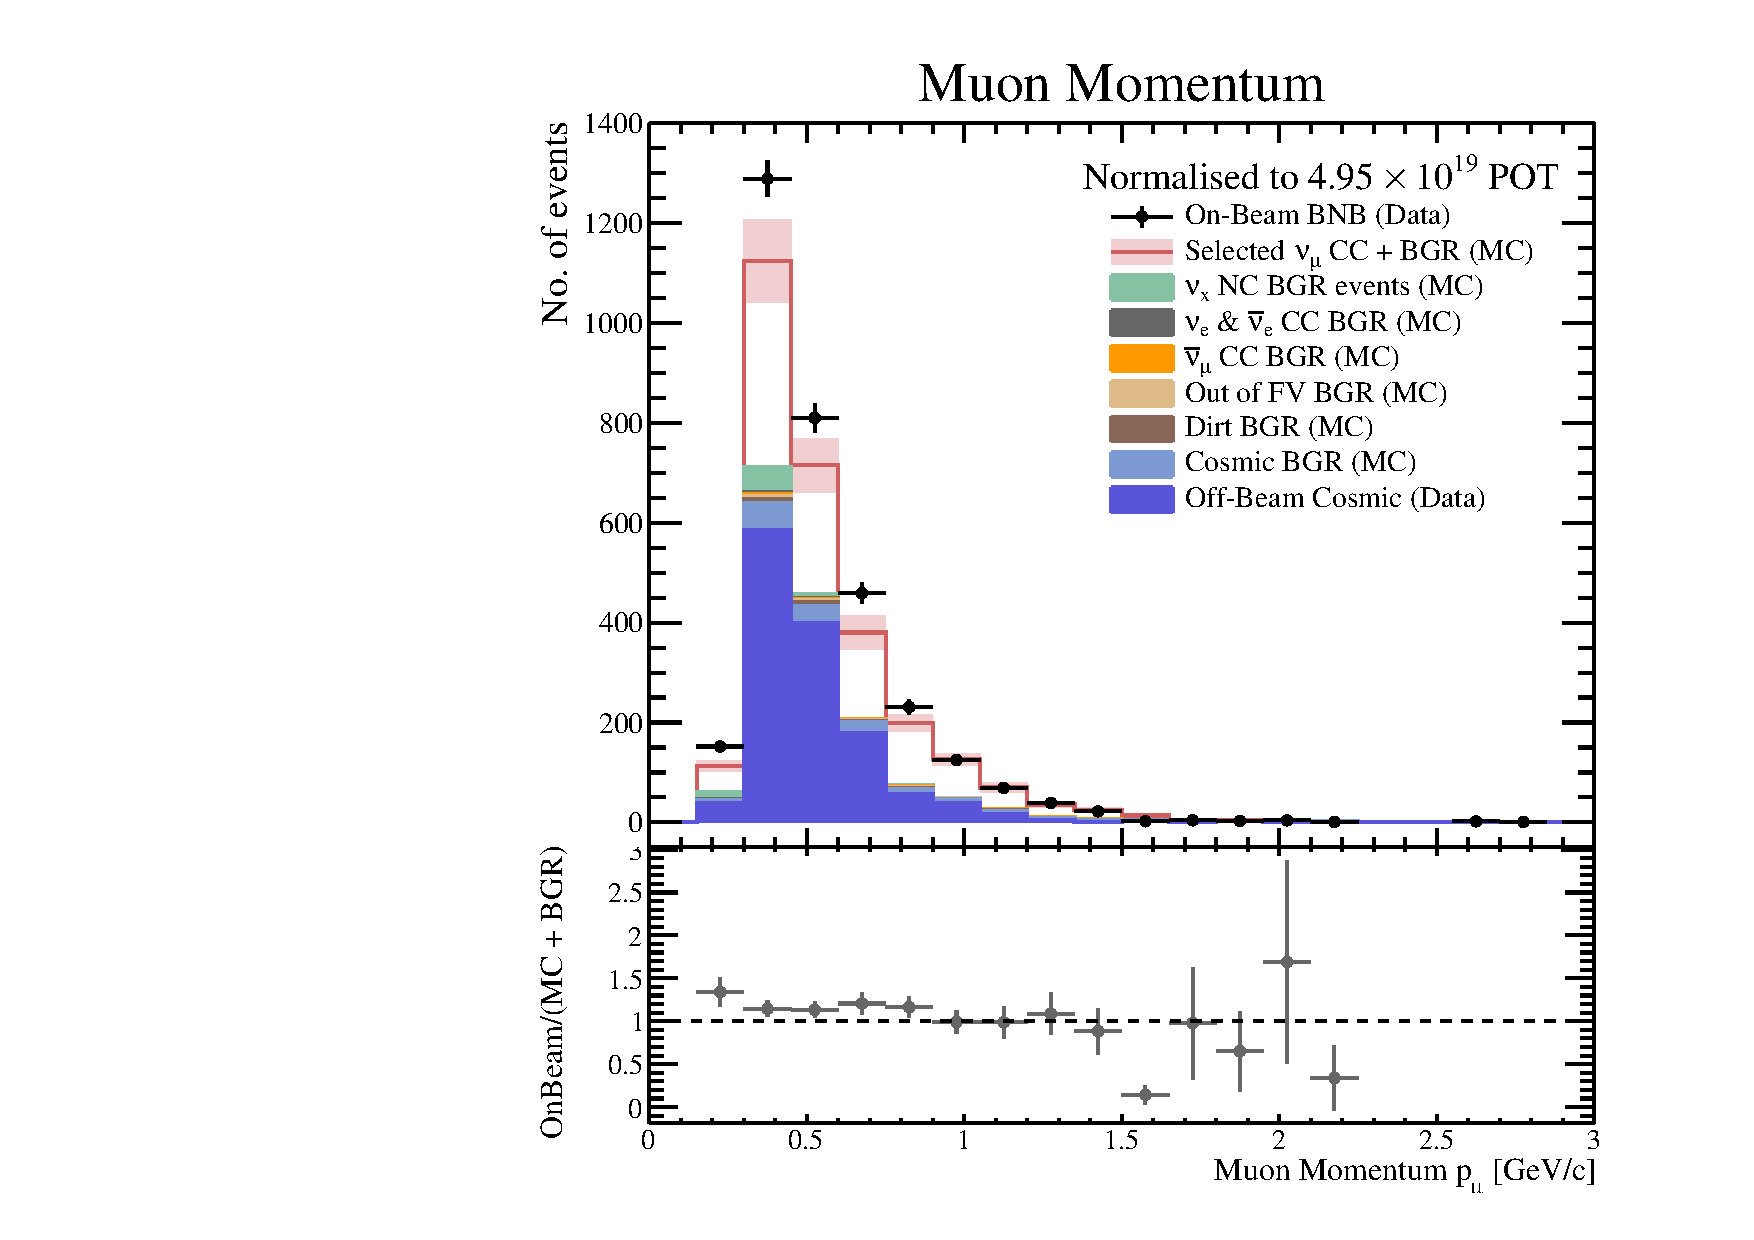
\includegraphics[width=0.8\textwidth]{images/FirstCCInclusive/Kinematic/ForwardFoldedMomentum.pdf}
    \caption[Forward-Folded Muon Momentum Distribution]{Depicted above we find the forward-folded muon momentum yield distribution in the interval $[0,3] \si{\giga\electronvolt}$.}
    \label{fig:ForwardFoldedMomentum}
\end{figure}
Figures \ref{fig:ForwardFoldedCosTheta} and \ref{fig:ForwardFoldedMomentum} show the two yield distributions which are commonly used to tune \gls{mc} generators like \gls{genie}. Namely, the $\cos{(\theta)}$ distribution and the muon momentum distribution. The $\cos{(\theta)}$ distribution also features an on-beam excess in the most forward bin, \ie towards $\cos{(\theta)} = 1$. These are also the bins with the highest statistics. It is also notable that the reducible and irreducible cosmic background is most dominant in the forward pointing bin. This is evidence that even rare cosmic-ray occurrences, like almost horizontal angles, are quite common compared to neutrino interactions in a neutrino beam. The muon momentum distribution is related to the track range distribution of figure \ref{fig:ForwardFoldedTrackRange}, although the transformation, from track range to track length and later on to momentum, is quite convoluted. Still, the two distributions bare some semblance. Also, here the bins with the most entries show an on-beam excess. 
%\textbf{Note to Michele: i should probably rebin the momentum distribution (1.5 to 3 GeV in one bin?). Advise is welcome!}

\begin{figure}[htbp]
    \centering
    \subfloat[][]
    {
        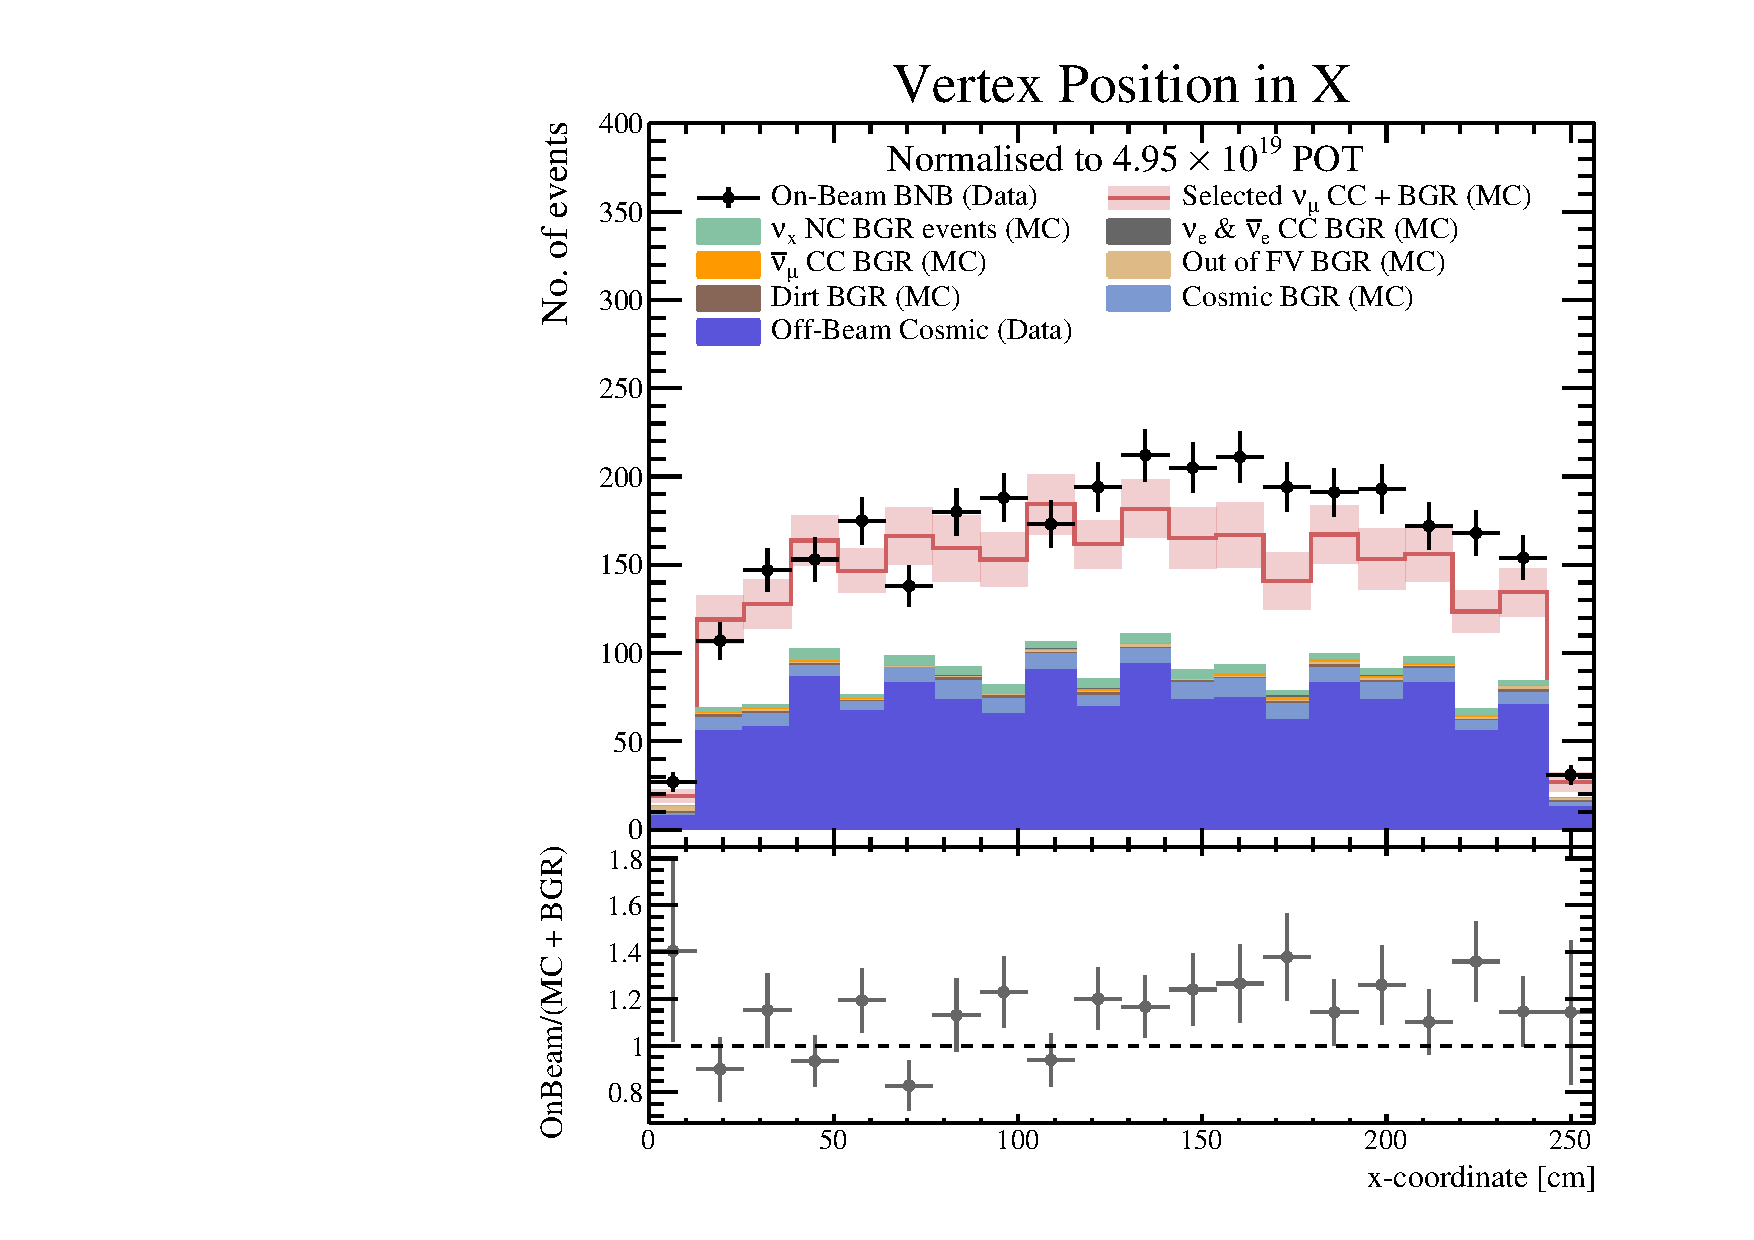
\includegraphics[width=0.32\textwidth]{images/FirstCCInclusive/Kinematic/ForwardFoldedXVtxPosition.pdf}
        \label{fig:ForwardFoldedXVtxPosition}
    }
    \subfloat[][]
    {
        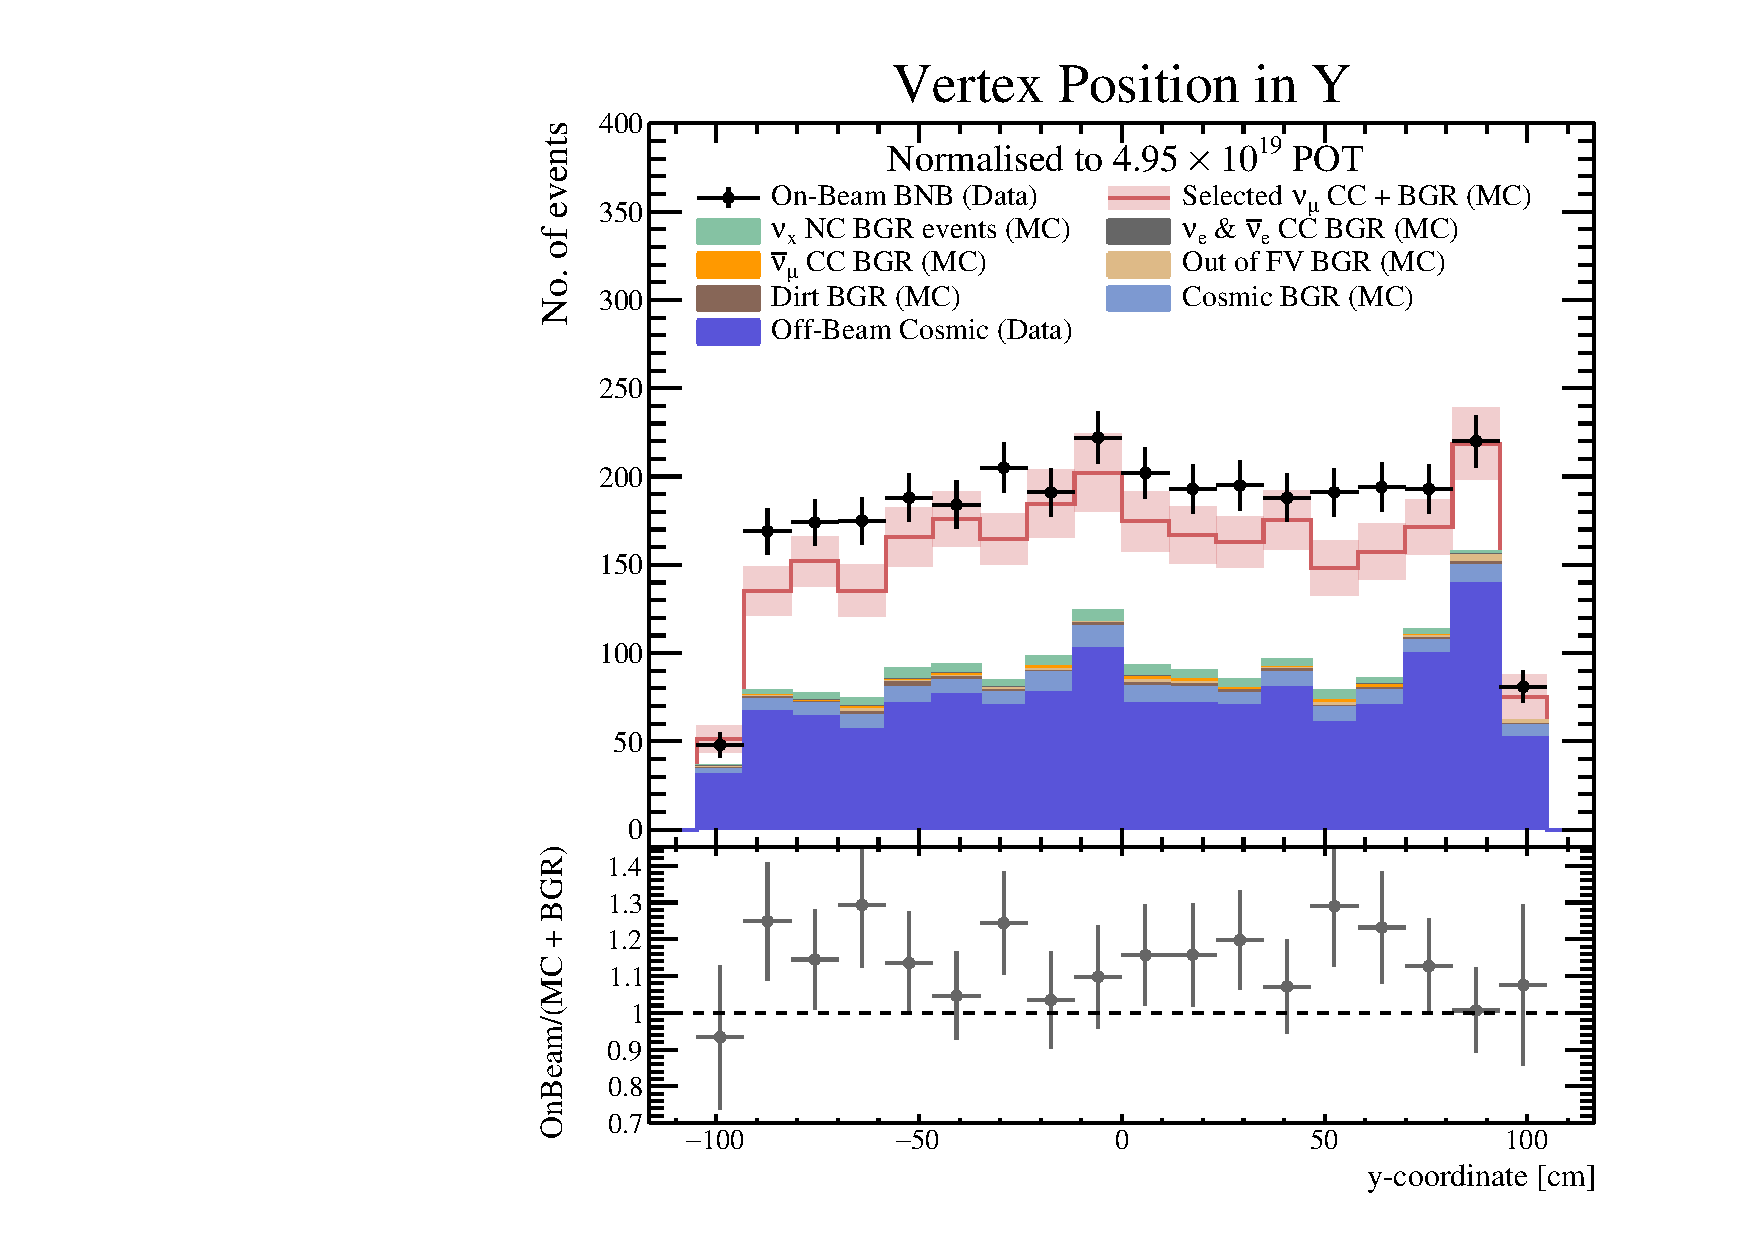
\includegraphics[width=0.32\textwidth]{images/FirstCCInclusive/Kinematic/ForwardFoldedYVtxPosition.pdf}
        \label{fig:ForwardFoldedYVtxPosition}
    }
    \subfloat[][]
    {
        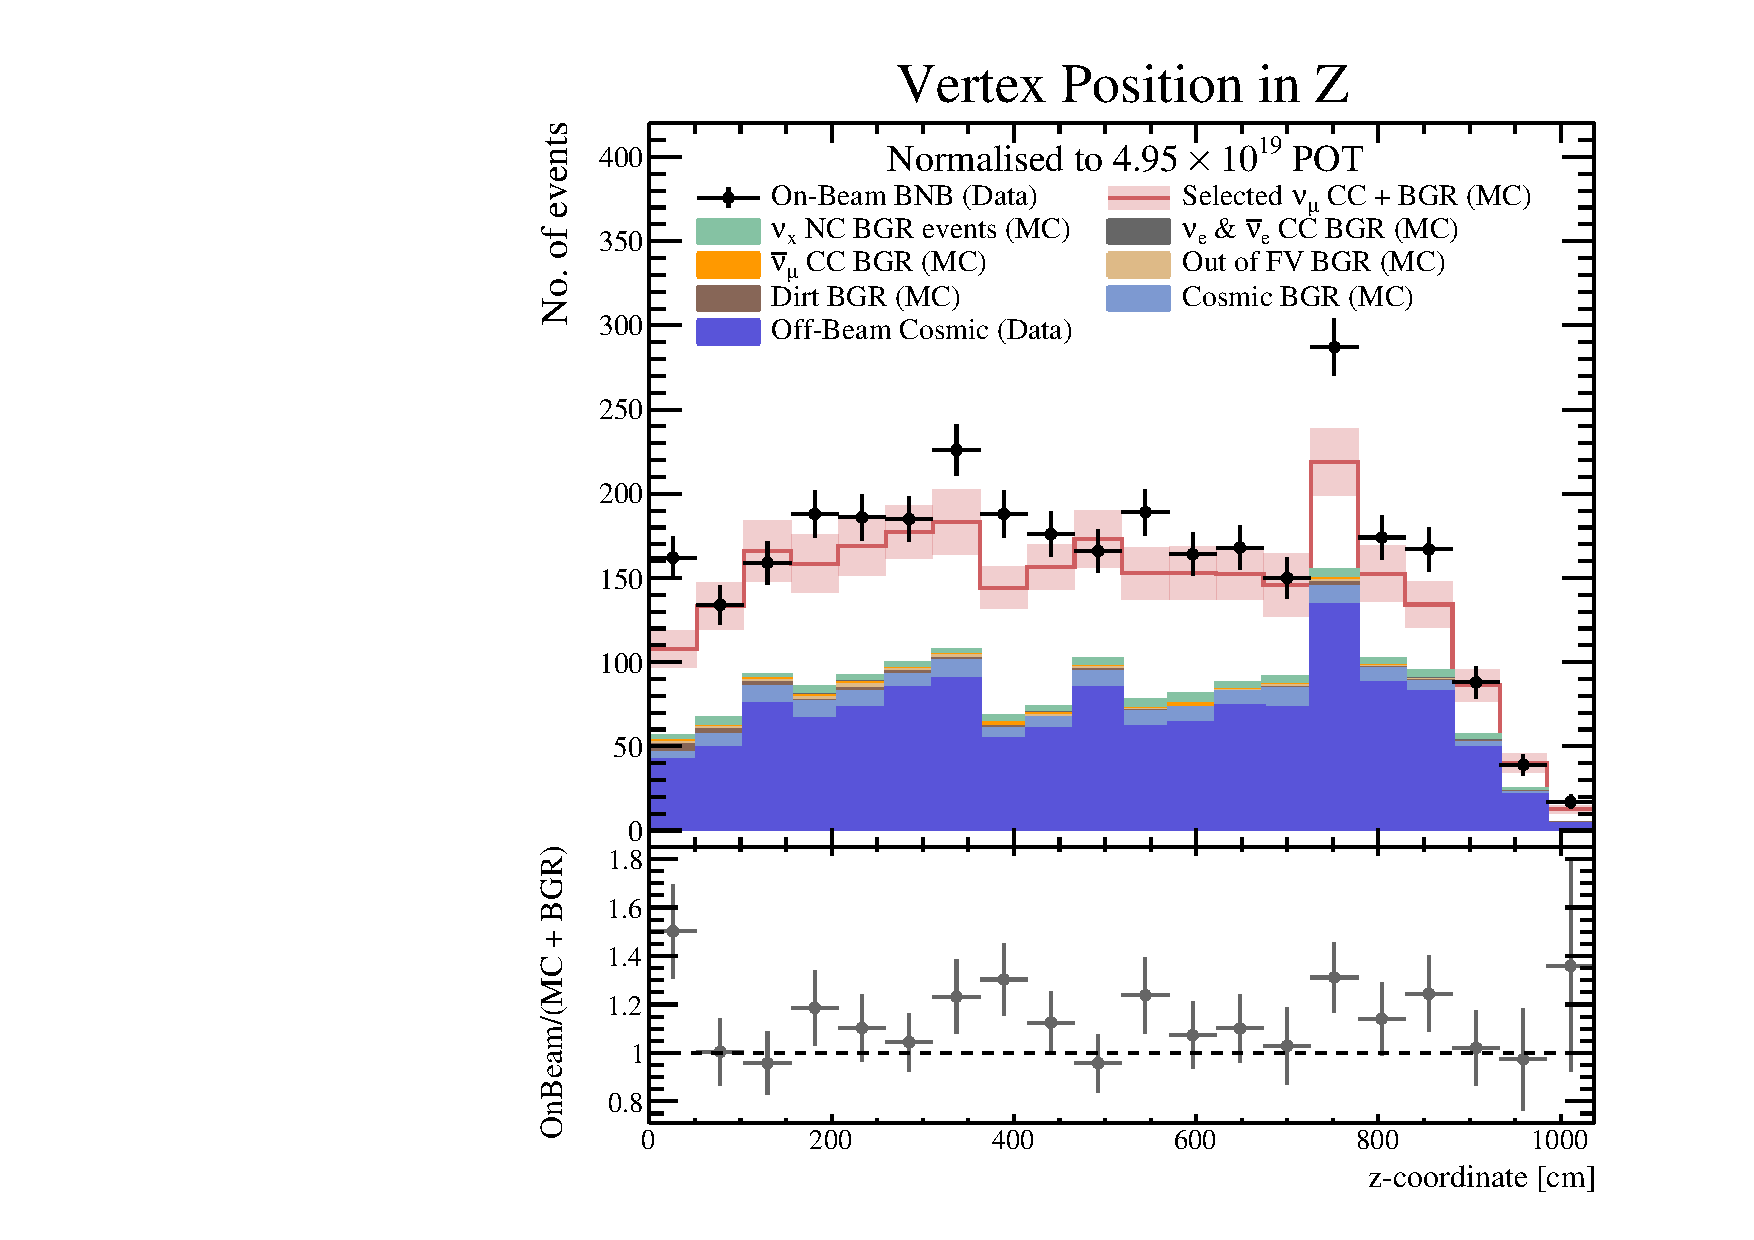
\includegraphics[width=0.32\textwidth]{images/FirstCCInclusive/Kinematic/ForwardFoldedZVtxPosition.pdf}
        \label{fig:ForwardFoldedZVtxPosition}
    }
    \caption[Forward-Folded Vertex Candidate Position Distributions]{Shown above are the forward-folded vertex candidate position distributions in all three dimensions. The respective histogram range is given by the active volume dimensions in the detector coordinates (see figure \ref{fig:MicroBooNECoordinateSystem}).}
    \label{fig:ForwardFoldedVertexPosition}
\end{figure}
Finally, the forward-folded vertex candidate position graphs are shown in figure \ref{fig:ForwardFoldedVertexPosition}. These are the cut variables of the \gls{fv} cut and hence feature bins with low content or even empty bins at both ends. The distributions of the $x$ and $z$ position coordinates are expected to be flat and their ratio plots are thus good indicators for the overall on-beam excess. The $y$ distribution, on the other hand, is expected to show increased cosmic activity towards the top. Another noteworthy feature of the $z$ distribution is the sudden increase of vertex candidates around $z=\SI{750}{\centi\metre}$, for on-beam as well as the \gls{mc} prediction. This can be attributed to a large dead wire region of the \gls{CollectionPlane} around the same coordinate, as shown in figure \ref{fig:DeadWires}. Tracks which traverse this area have a higher chance to be reconstructed as two tracks, because of the introduced discontinuity. The reconstruction software perceives a vertex at the start of the putative track, beginning at the dead wire gap.

Overall, it can be stated that the baseline \gls{mc} model is not an adequate representation of this measurement. But what about the other models? To answer this question I compared the on-beam sample to the forward-folded predictions of the \gls{bnb} \textbf{M\textsubscript{A}\num{1.35}}, \gls{bnb} \gls{esf}\&\gls{tem}, and \gls{bnb} \gls{mec} samples. In the following graphs, their distributions are overlayed with each other and the on-beam data. The forward-folded $\cos{(\theta)}$ is shown in figure \ref{fig:ModelComparisonCosTheta} and the forward-folded momentum distribution in figure \ref{fig:ModelComparisonMomentum}.

\begin{figure}[htbp]
    \centering
    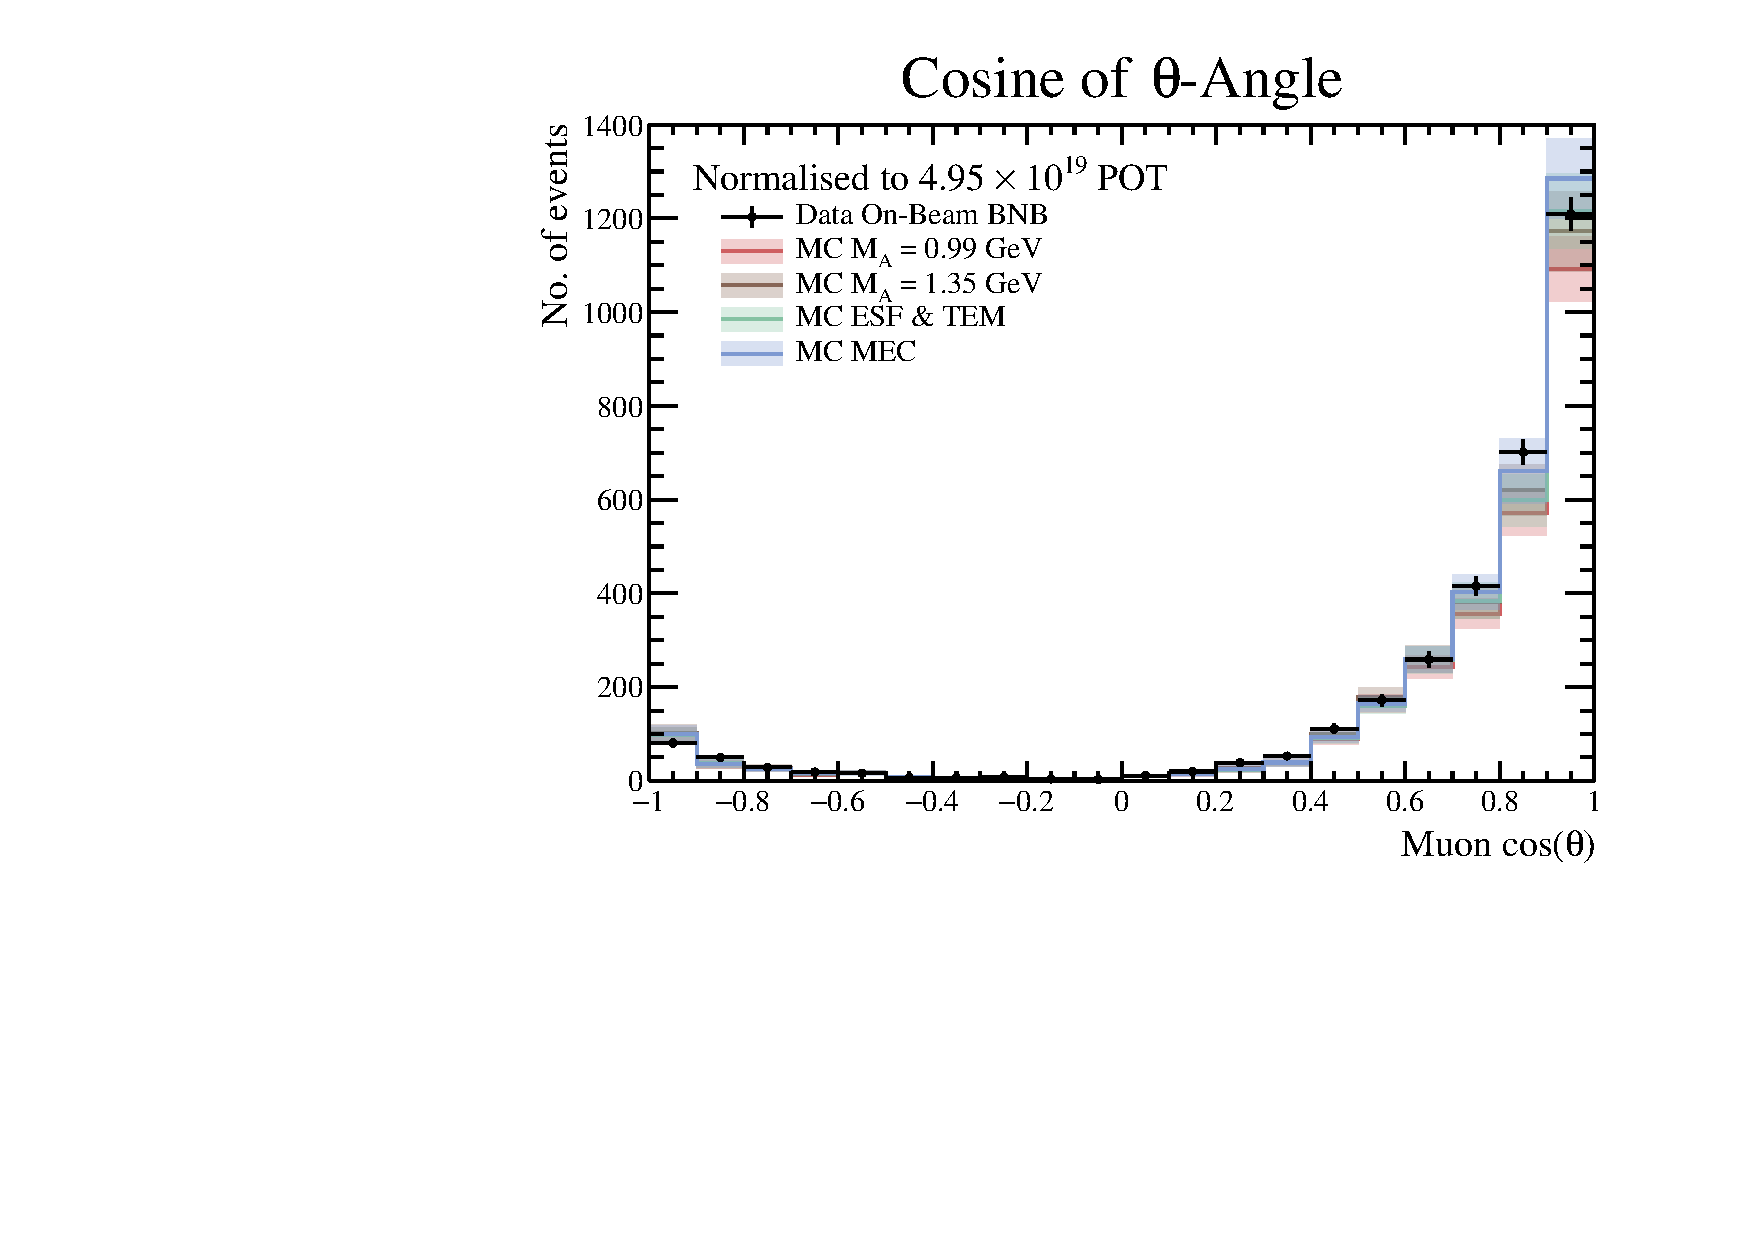
\includegraphics[width=0.8\textwidth]{images/FirstCCInclusive/ModelComparison/ModelComparisonCosTheta.pdf}
    \caption[Model Comparison $\cos{(\theta)}$ Distribution]{Depicted here, is the forward-folded $\cos{(\theta)}$ yield distribution in the full interval $[-1,1]$. The on-beam data is shown together with the four \gls{mc} models introduced in section \ref{sec:MCSamples}.}
    \label{fig:ModelComparisonCosTheta}
\end{figure}
\begin{figure}[htbp]
    \centering
    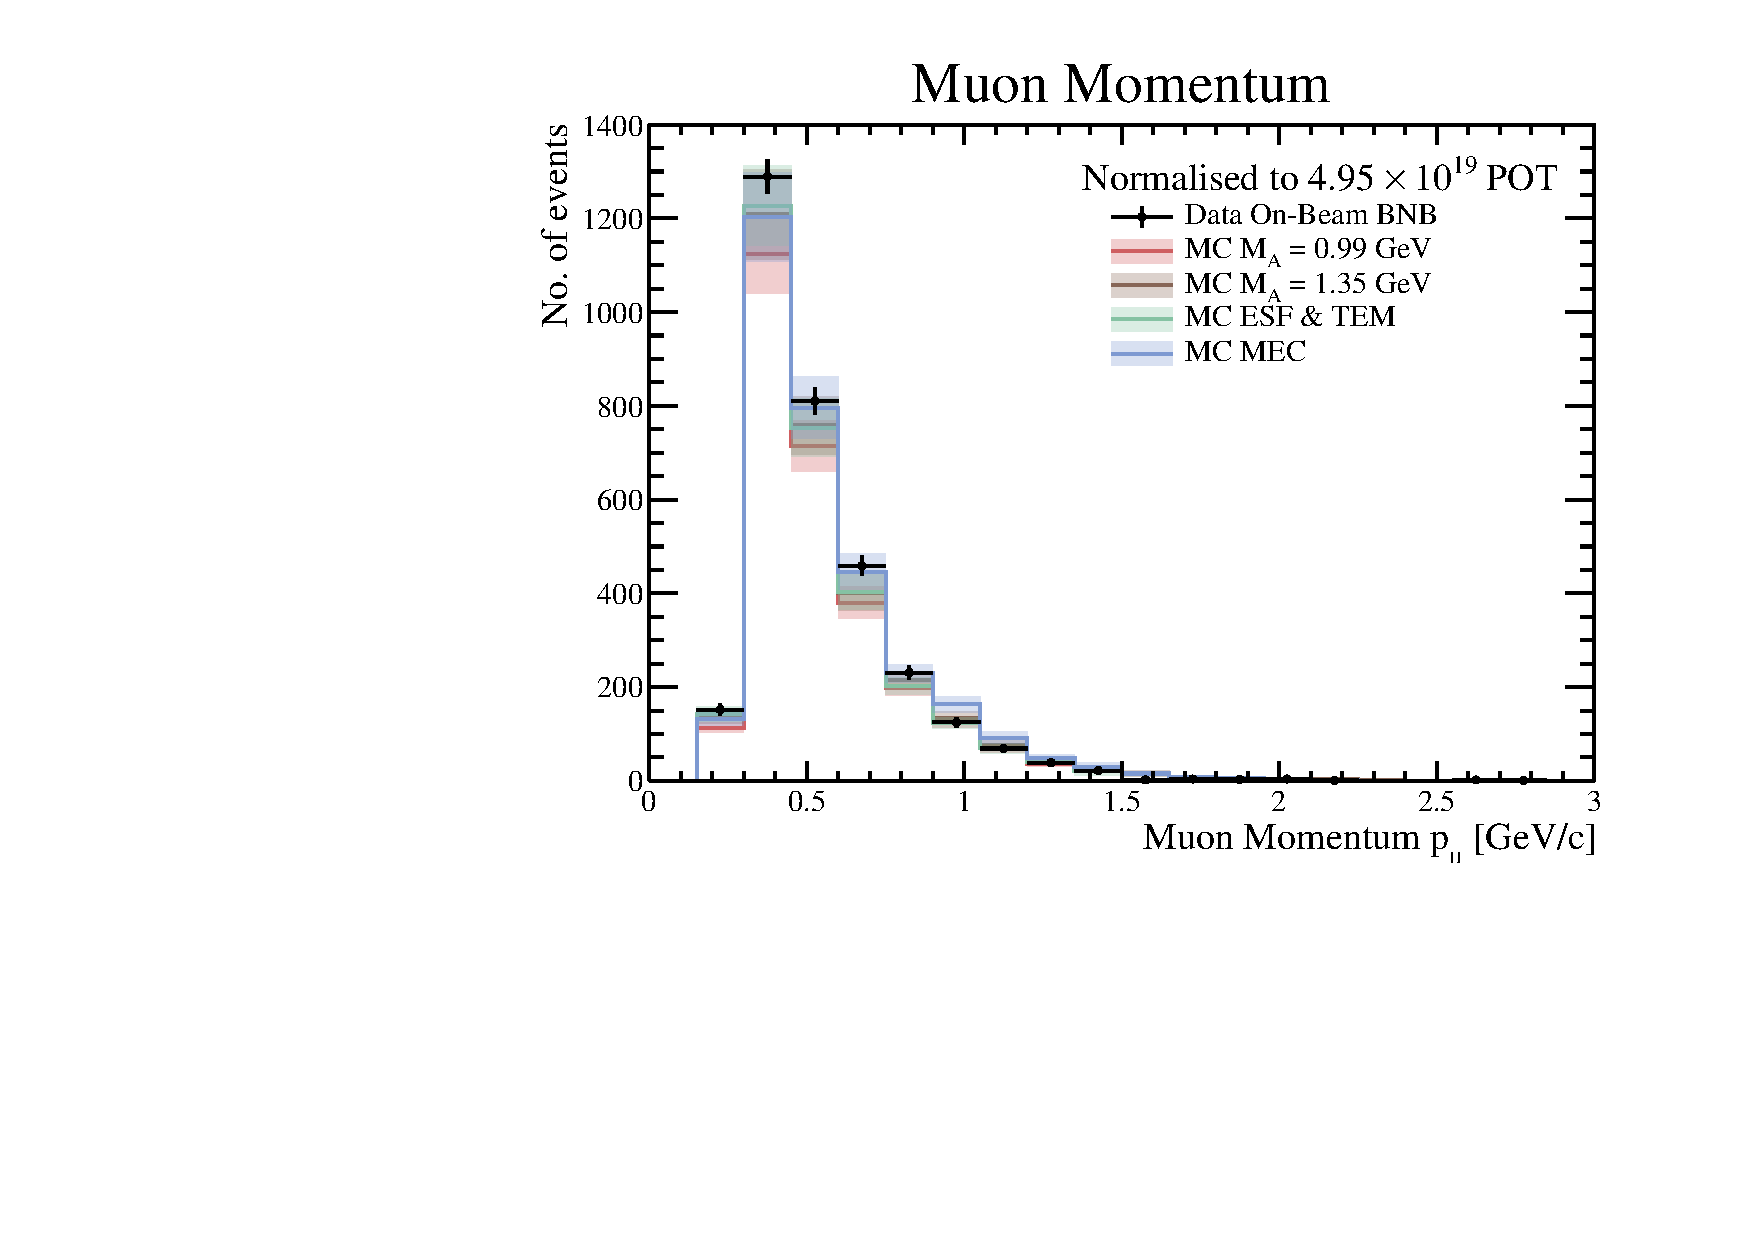
\includegraphics[width=0.8\textwidth]{images/FirstCCInclusive/ModelComparison/ModelComparisonMomentum.pdf}
    \caption[Model Comparison Muon Momentum Distribution]{Depicted above we find the forward-folded muon momentum yield distribution in the interval $[0,3] \si{\giga\electronvolt}$. Here, the on-beam data is compared to the four models used in this analysis (see in section \ref{sec:MCSamples}).}
    \label{fig:ModelComparisonMomentum}
\end{figure}
Generally, it can be stated that all additional models are in better agreement with the measurement than the baseline sample. The data points are almost all within reach of the respective error bands, except in the case of the baseline model. However, it is hard to make more qualitative statements, for the uncertainties of this analysis are too great. A list of $\chi^2/\text{NDF}$ is provided in table \ref{tab:ChiSquareTest}. They are calculated using a method of comparing unweighted (on-beam) to weighted (\gls{mc} prediction) histograms. This method is provided by ROOT and documented in \cite{ChiSquareTest1,ChiSquareTest2}. Using $\chi^2/\text{NDF}$ as quality of match indicator, the combined \gls{esf}\&\gls{tem} seems to be the best representation for the measured $\cos{(\theta)}$, while the $M_A=\num{1.35}$ model best matches the measured muon momentum distribution. Considering both distributions together, \gls{esf}\&\gls{tem} represents the best match for this measurement by far. Note, that due to the low statistics of this analysis the $\chi^2/\text{NDF}$ should not be used to assess the overall quality of the models.
\begin{table}[htbp]
    \centering
    \caption[$\chi^2$-Tests of MC Models]{Listed below are the $\chi^2/\text{NDF}$ of the different models. The values were calculated according to \cite{ChiSquareTest1,ChiSquareTest2}.}
    \begin{tabu}{lrrrr}
        \toprule
        \rowfont[c]{\bf} Distribution & Baseline & M\textsubscript{A}\num{1.35} & \gls{tem} & \gls{mec}\\
        \midrule
        Muon $\cos{(\theta)}$ & \num{0.79} & \num{0.48} & \num{0.98} & \num{0.94} \\
        Muon momentum & \num{1.36} & \num{0.89} & \num{1.15} & \num{2.09} \\
        \bottomrule
        \label{tab:ChiSquareTest}
    \end{tabu}
\end{table}

\subsection{Detector Smearing} \label{sec:DetectorSmearing}
The detector and reconstruction effects can be visualised by so-called \textbf{smearing matrices}, $U$. A smearing matrix serves as an instrument to translate true into reconstructed kinematic distributions. This is done in a linear way,
\begin{equation}
    \nu_i = \sum_{j=1}^{n} U_{ij} \mu_j,
\end{equation}
with $\nu_i$ denoting the content of reconstruction bin $i$, and $\mu$ the content of true bin $j$. The matrix elements $U_{ij}$ is given by the probability of a true bin entry to be observed as a certain reconstructed bin entry, \ie
\begin{equation}
    U_{ij} = P\left( \text{observed in bin } i \mid \text{true value in bin } j\right).
\end{equation}
In this analysis, the smearing matrices are created as \gls{2d} histograms. Said histograms are filled with the reconstructed and true properties of the selected events provided by the \gls{mc} baseline sample. Naturally, the matrices are conceived in the dimensions $n \times n$, with $n$ being the same as the number of bins of their associated kinematic distribution. A range of notable smearing matrices is shown below in figures \ref{fig:DiagonalSmearing} through \ref{fig:SmearingMatrixMomentum}.
\begin{figure}[htbp]
    \centering
    \subfloat[][]
    {
        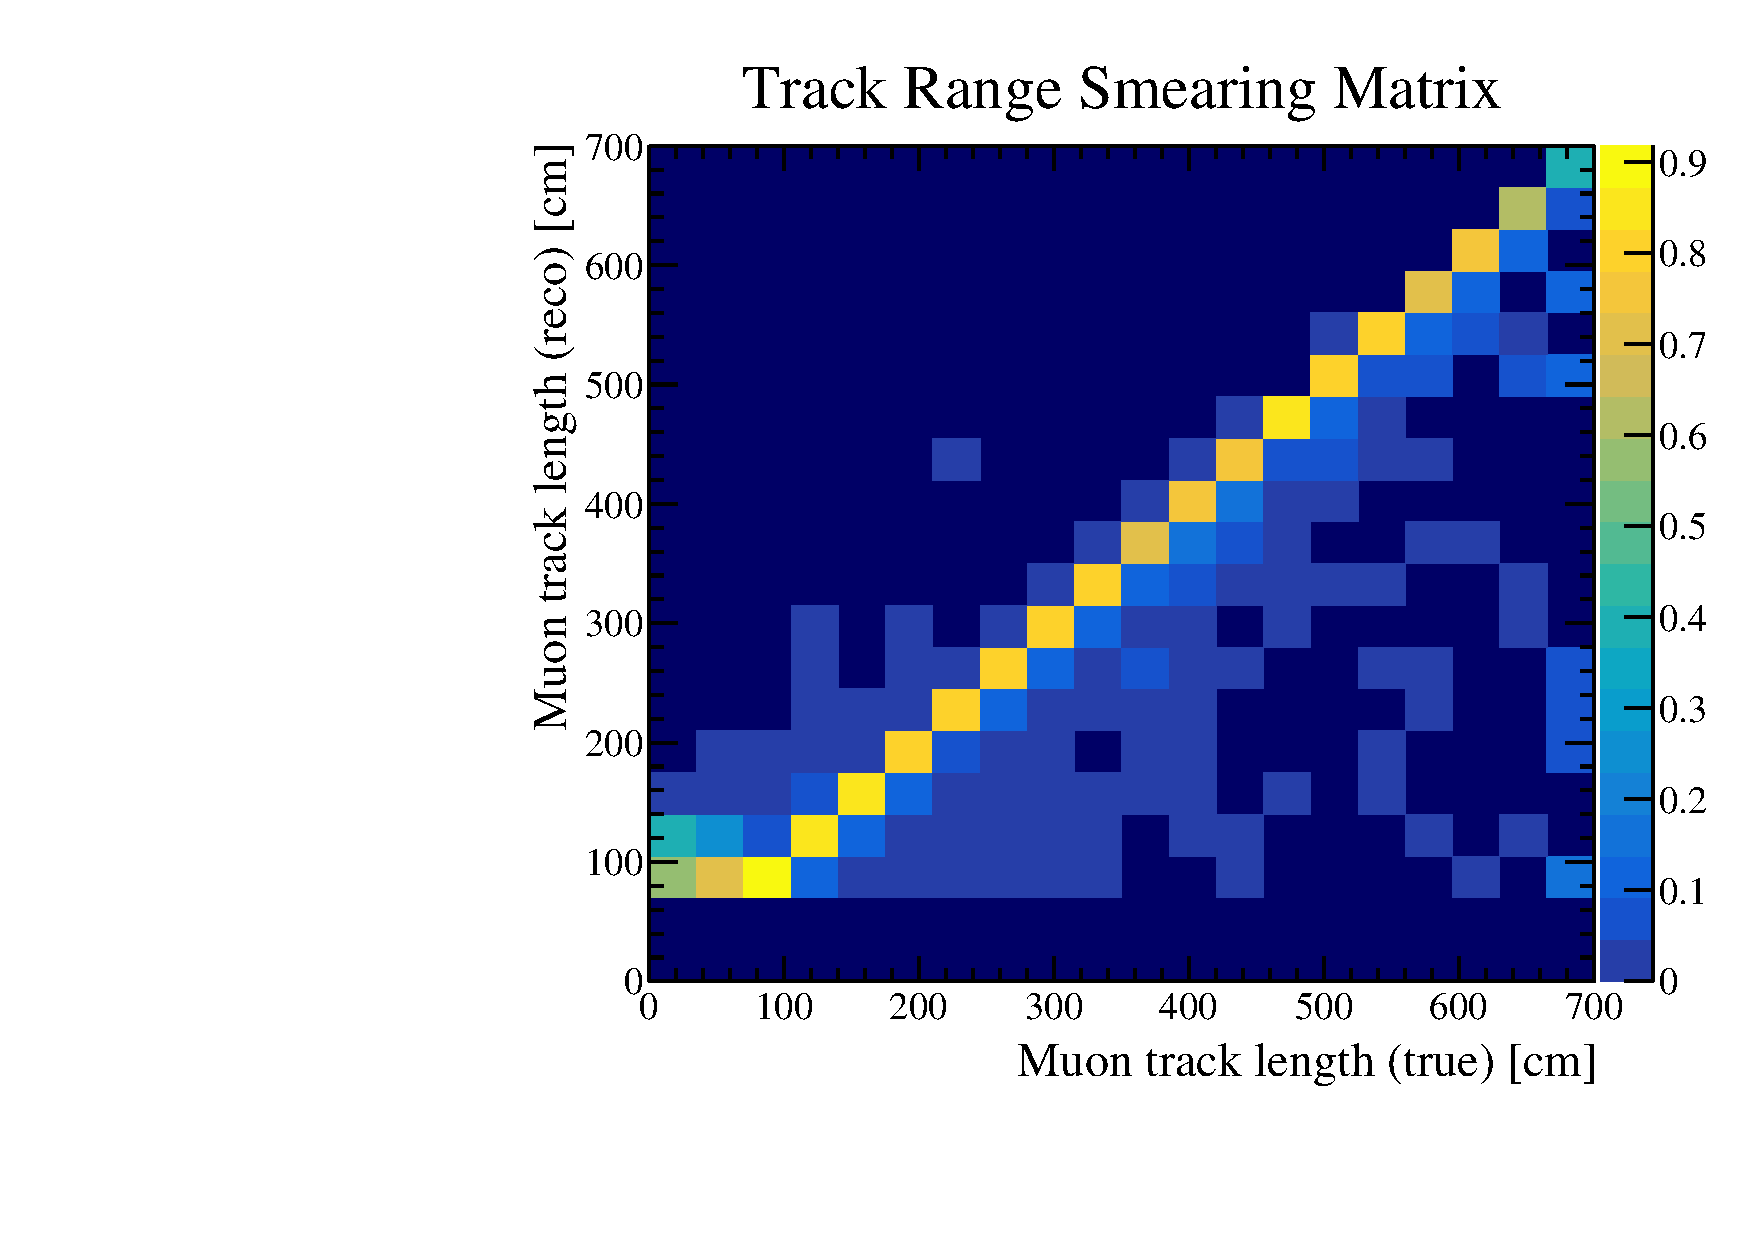
\includegraphics[width=0.48\textwidth]{images/FirstCCInclusive/Smearing/SmearingMatrixTrackRange.pdf}
        \label{fig:SmearingMatrixTrackRange}
    }
    \subfloat[][]
    {
        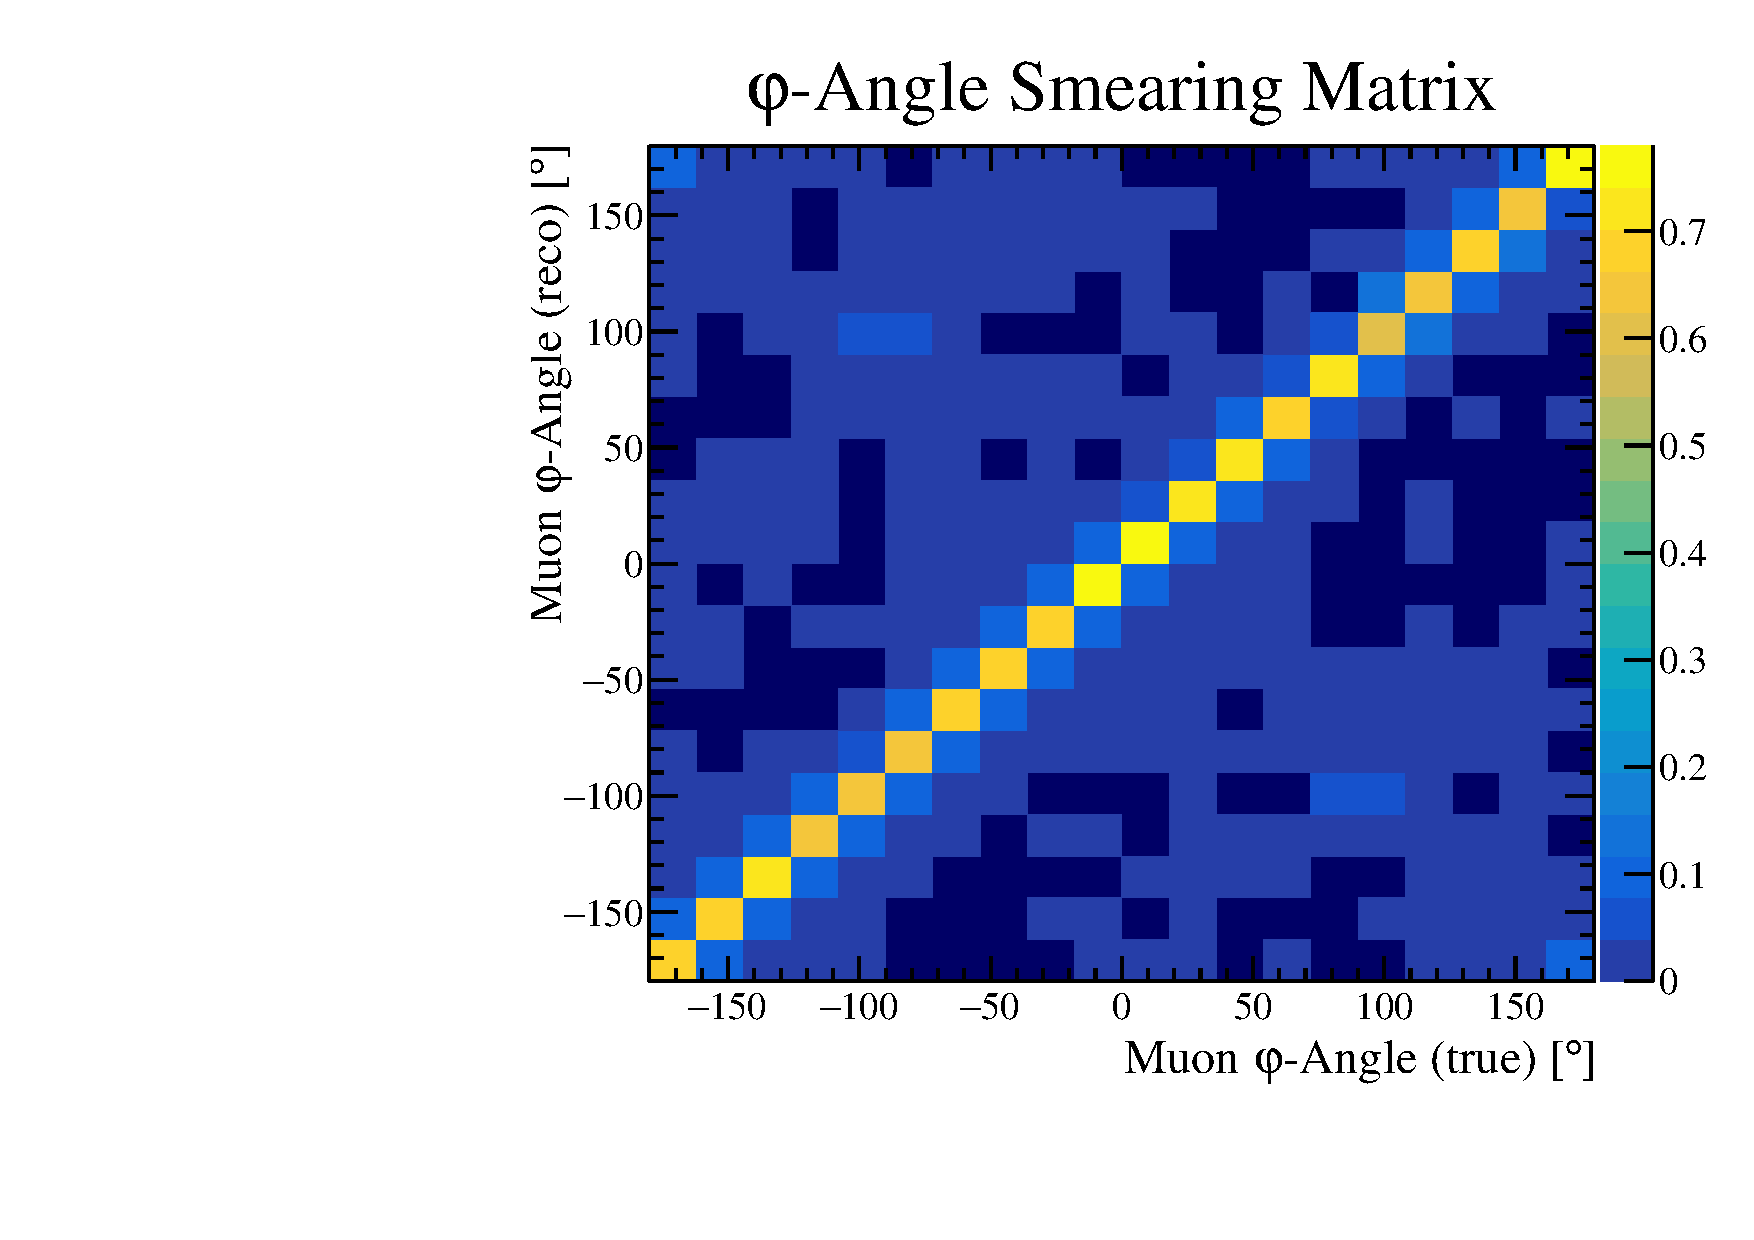
\includegraphics[width=0.48\textwidth]{images/FirstCCInclusive/Smearing/SmearingMatrixPhi.pdf}
        \label{fig:SmearingMatrixPhi}
    }
    \caption[Smearing Matrices of Track Range and $\phi$ Distributions]{Shown above are the smearing matrices of the track range distribution \subref{fig:SmearingMatrixTrackRange}, and $\phi$-angle distributions \subref{fig:SmearingMatrixPhi}. Both matrices show diagonal behaviour, although there is strong smearing at low track ranges. Moreover, the track range cut causes zero entries in the first two reconstruction bins.}
    \label{fig:DiagonalSmearing}
\end{figure}

Ideally, these matrices should be almost diagonal, as this is an indicator for high reconstruction and selection coherence. In this analysis, diagonality can be observed in the vertex positions (not shown in any figures), the $\phi$-angle in figure \ref{fig:SmearingMatrixPhi}, and to a lesser degree also for the track range smearing matrices \ref{fig:SmearingMatrixTrackRange}. The latter shows strong smearing for ranges below \SI{100}{\centi\metre}. The $\cos{(\theta)}$ matrix in figure \ref{fig:SmearingMatrixCosTheta} shows an interesting V-shaped feature. It seems that the muon track candidates get preferably reconstructed in forward direction, even if they are directed backwards. This effect is not caused by the selection, since the value of $\theta$ is given by \gls{Pandora}. At last, the muon momentum smearing matrix is shown in figure \ref{fig:SmearingMatrixMomentum}. This matrix is mostly diagonal between \SIlist[per-mode = symbol]{0.3;1.5}{\giga\electronvolt\per\lightspeed}. Below this range, the smearing shows similar behaviour as in the track range matrix. Above  \SI[per-mode = symbol]{1.5}{\giga\electronvolt\per\lightspeed} the momenta get completely misreconstructed to the point where one could barely call it smearing anymore. However, it has to be stated, that these atypical occurrences are seen in areas with very low statistics and are dominated by cosmic activity. For reference, consider the corresponding forward-folded distribution in figure \ref{fig:ForwardFoldedMomentum}.
\begin{figure}[htbp]
    \centering
    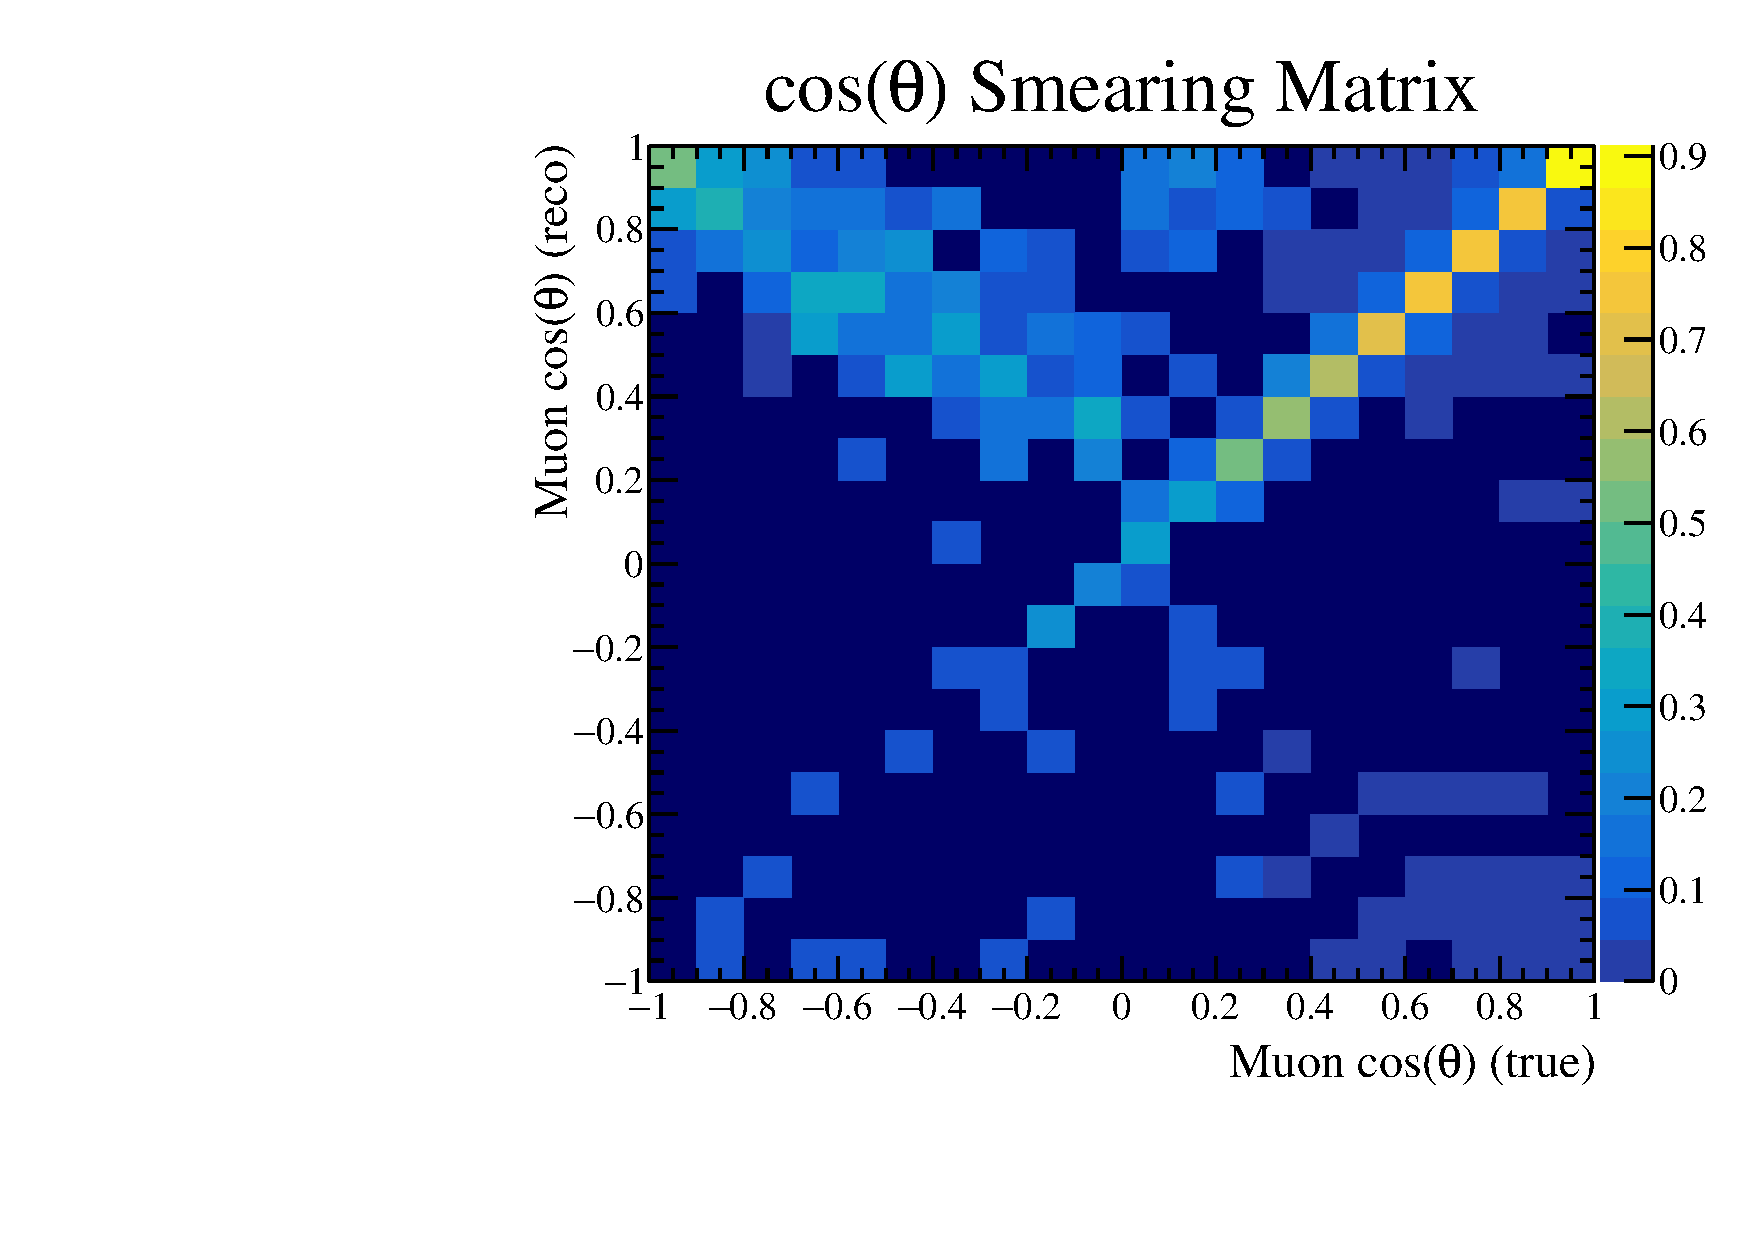
\includegraphics[width=0.8\textwidth]{images/FirstCCInclusive/Smearing/SmearingMatrixCosTheta.pdf}
    \caption[Smearing Matrices of the $\cos{(\theta)}$ Distribution]{The smearing matrix of the $\cos{(\theta)}$ distribution is presented here. This matrix features a v-shaped due to \gls{Pandora}'s preference of forward reconstructing tracks.}
    \label{fig:SmearingMatrixCosTheta}
\end{figure}
\begin{figure}[htbp]
    \centering
    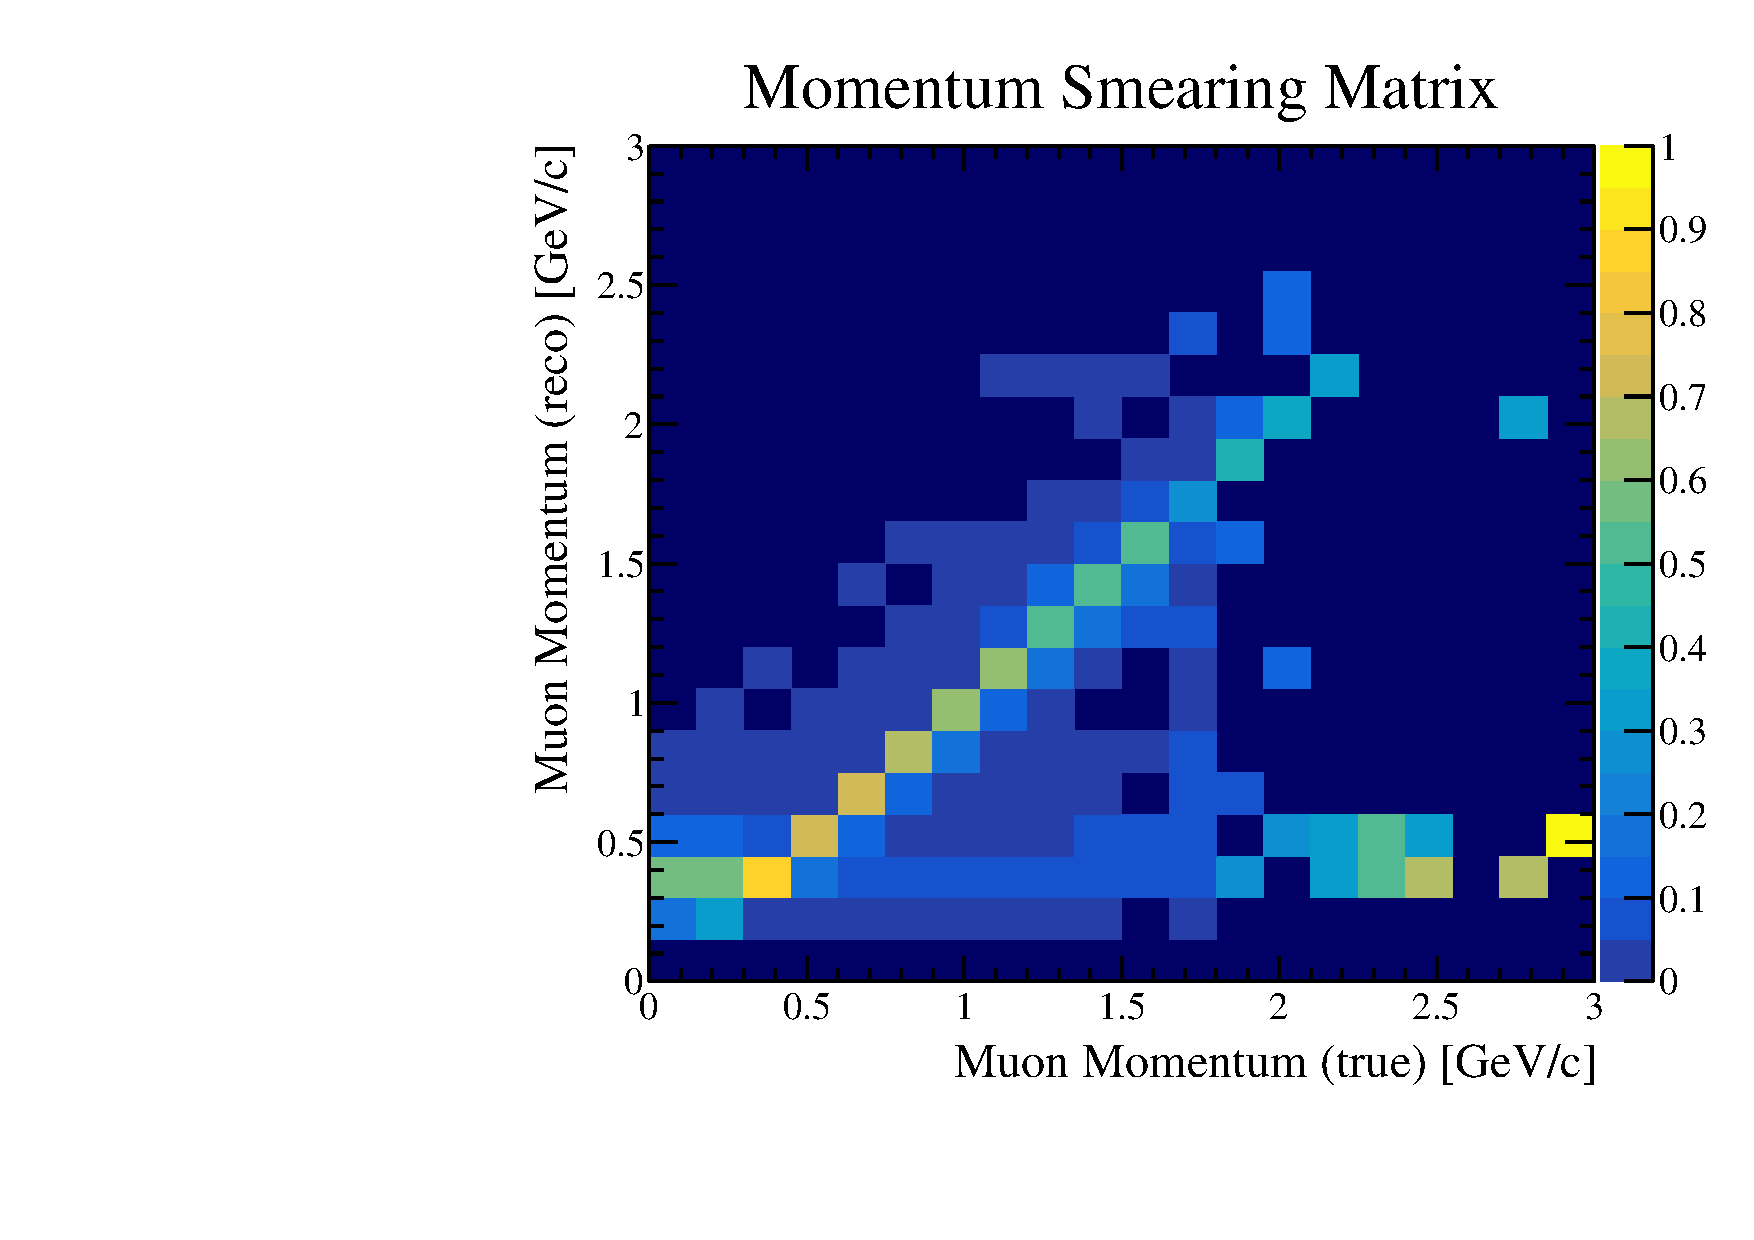
\includegraphics[width=0.8\textwidth]{images/FirstCCInclusive/Smearing/SmearingMatrixMomentum.pdf}
    \caption[Smearing Matrices of the Momentum Distribution]{Depicted above, is the smearing matrix of the momentum distribution. This matrix seems to be diagonal between \SIrange[per-mode = symbol]{0.3}{1.5}{\giga\electronvolt\per\lightspeed}. However, there are a lot of true high-momentum events which reconstructed at quite low momenta. This is mostly due to cosmic background, where the track is not fully contained within the active volume.}
    \label{fig:SmearingMatrixMomentum}
\end{figure}

\subsection{Systematic Uncertainties} \label{sec:Systematics}
Early in this analysis, we recognised remnants of cosmic-ray related event signatures \cite{MicroBooNECCInclIN}. This was most prominently prevalent in the shape of the $\phi$ and $\theta$ distributions. My modifications to the selection process reduced these cosmic features, although it is still notable in the kinematic $\phi$ in figure \ref{fig:ForwardFoldedPhi}. There, an increase in on-beam events with $\phi \approx \pm \SI{90}{\degree}$ can be observed. These signatures are linked to the simulated cosmic pileup background, which seems to exhibit notable differences to real measured cosmic events. This prompted me to investigate these distributions further, using a subset of off-beam data and the \gls{mc} inTime cosmic sample. Both these samples are meant to be equivalent and can thus be scaled by their respective number of events. Furthermore, I considered both reconstruction passes, pandoraCosmic and pandoraNu (for reference consult section \ref{sec:EventReconstruction}). A simple comparison of the track reconstruction yield per event, listed in table \ref{tab:CosmicTrackReco}, already shows discrepancies. The difference between off-beam and inTime samples is almost \SI{20}{\percent} in pandoraCosmic, while in pandoraNu said difference at around \SI{5}{\percent} seems comparatively marginal.
\begin{table}[htbp]
    \centering
    \caption[Cosmic-Ray Track Reconstruction Yields]{Listed below are the tack reconstruction yields of the off-beam BNBEXT and inTime cosmic after the pandoraCosmic and pandoraNu reconstruction passes. The yield shows how many tracks are reconstructed per trigger event.}
    \begin{tabu}{lrr}
        \toprule
        \rowfont[c]{\bf} Sample Name & pandoraCosmic & pandoraNu \\
        \midrule
        off-beam BNBEXT & \num{39.1(12)} & \num{6.36(21)} \\
        inTime cosmic & \num{47.6(7)} & \num{6.60(10)} \\
        \bottomrule
        \label{tab:CosmicTrackReco}
    \end{tabu}
\end{table}
This seems very odd, but track reconstruction is also a very convoluted process, able to show non-linear behaviour. In the end, we are interested in distributions in order to quantify the uncertainty caused by data-\gls{mc} differences. The most crucial ones, regarding cosmic activity, are the angular distributions. These are shown in figures \ref{fig:CosmicRecoPhi} and \ref{fig:CosmicRecoCosTheta}.
\begin{figure}[htbp]
    \centering
    \subfloat[][]
    {
        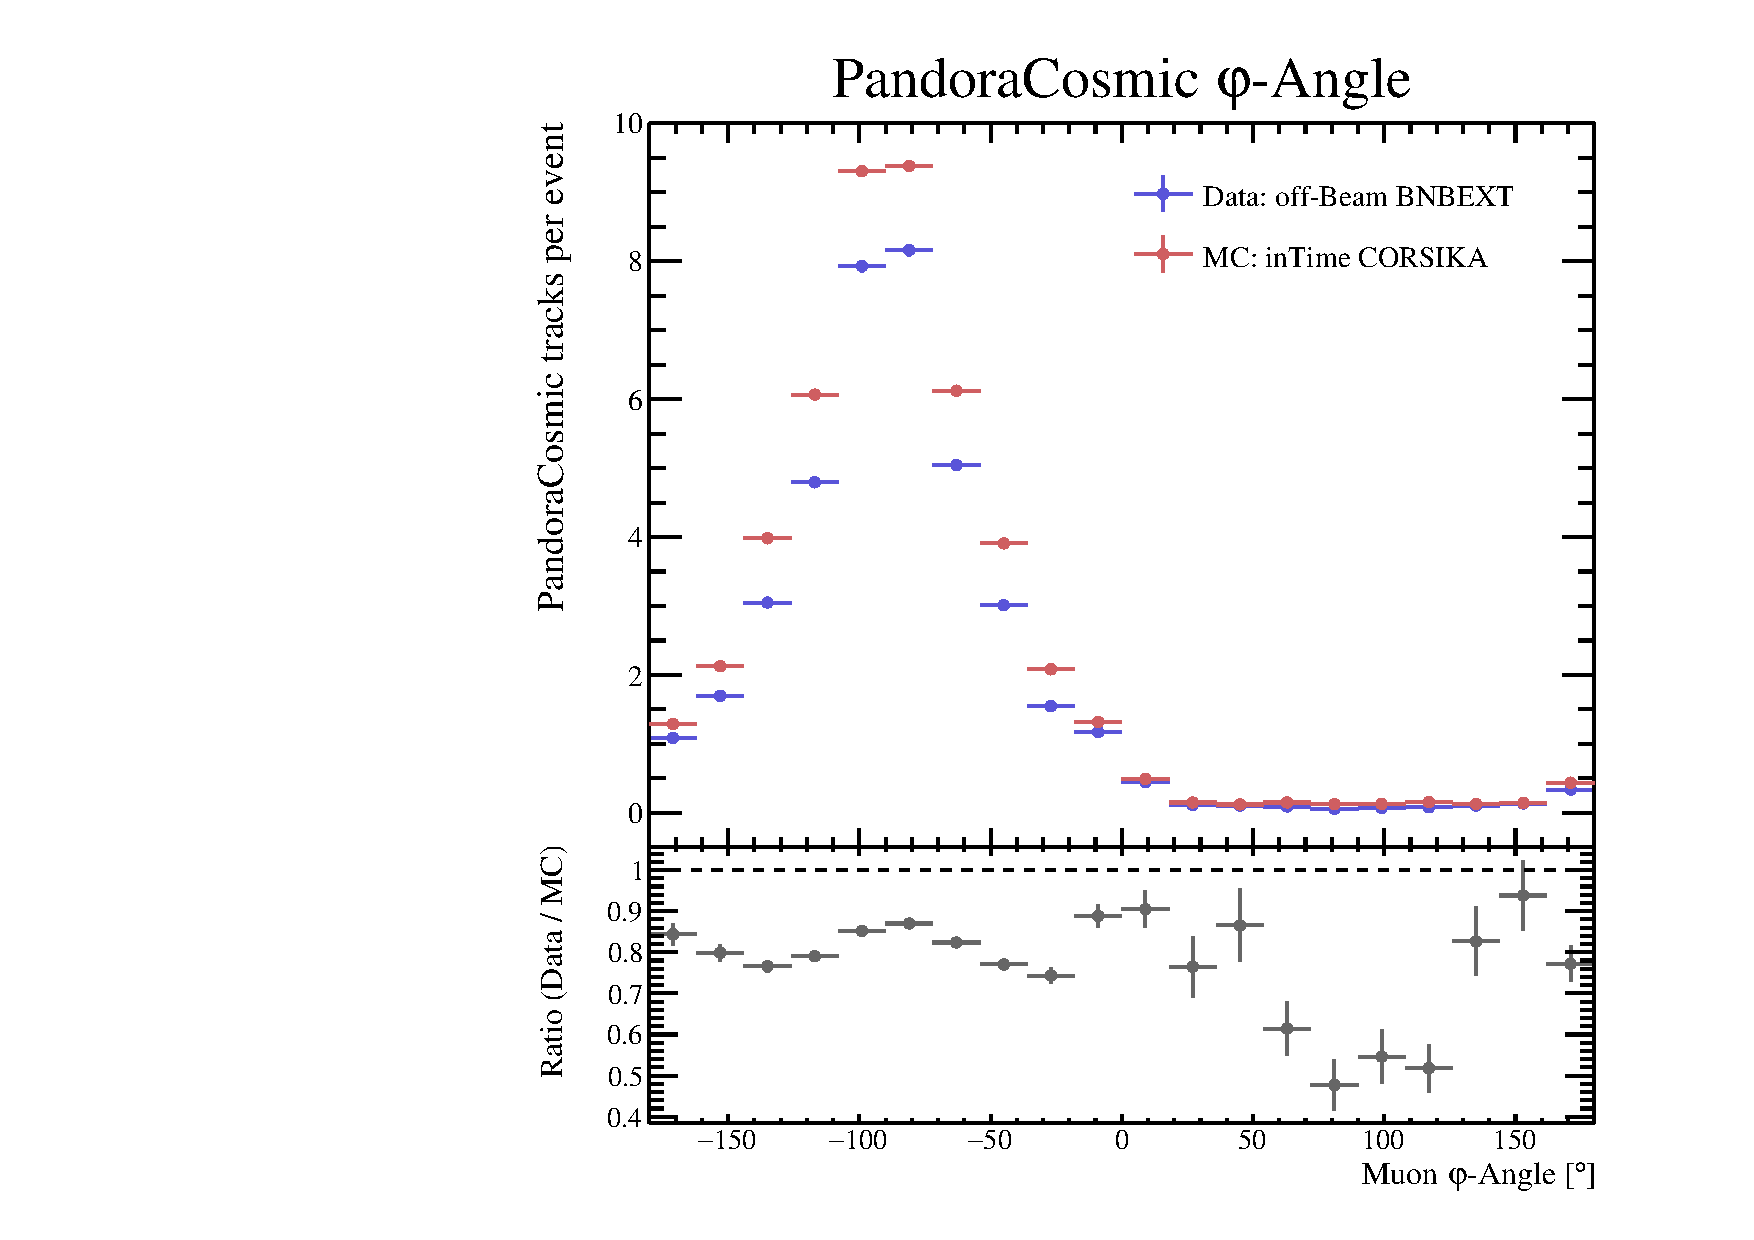
\includegraphics[width=0.5\textwidth]{images/FirstCCInclusive/CosmicBackground/CosmicPhiPandoraCosmic.pdf}
        \label{fig:PhiPandoraCosmic}
    }
    \subfloat[][]
    {
        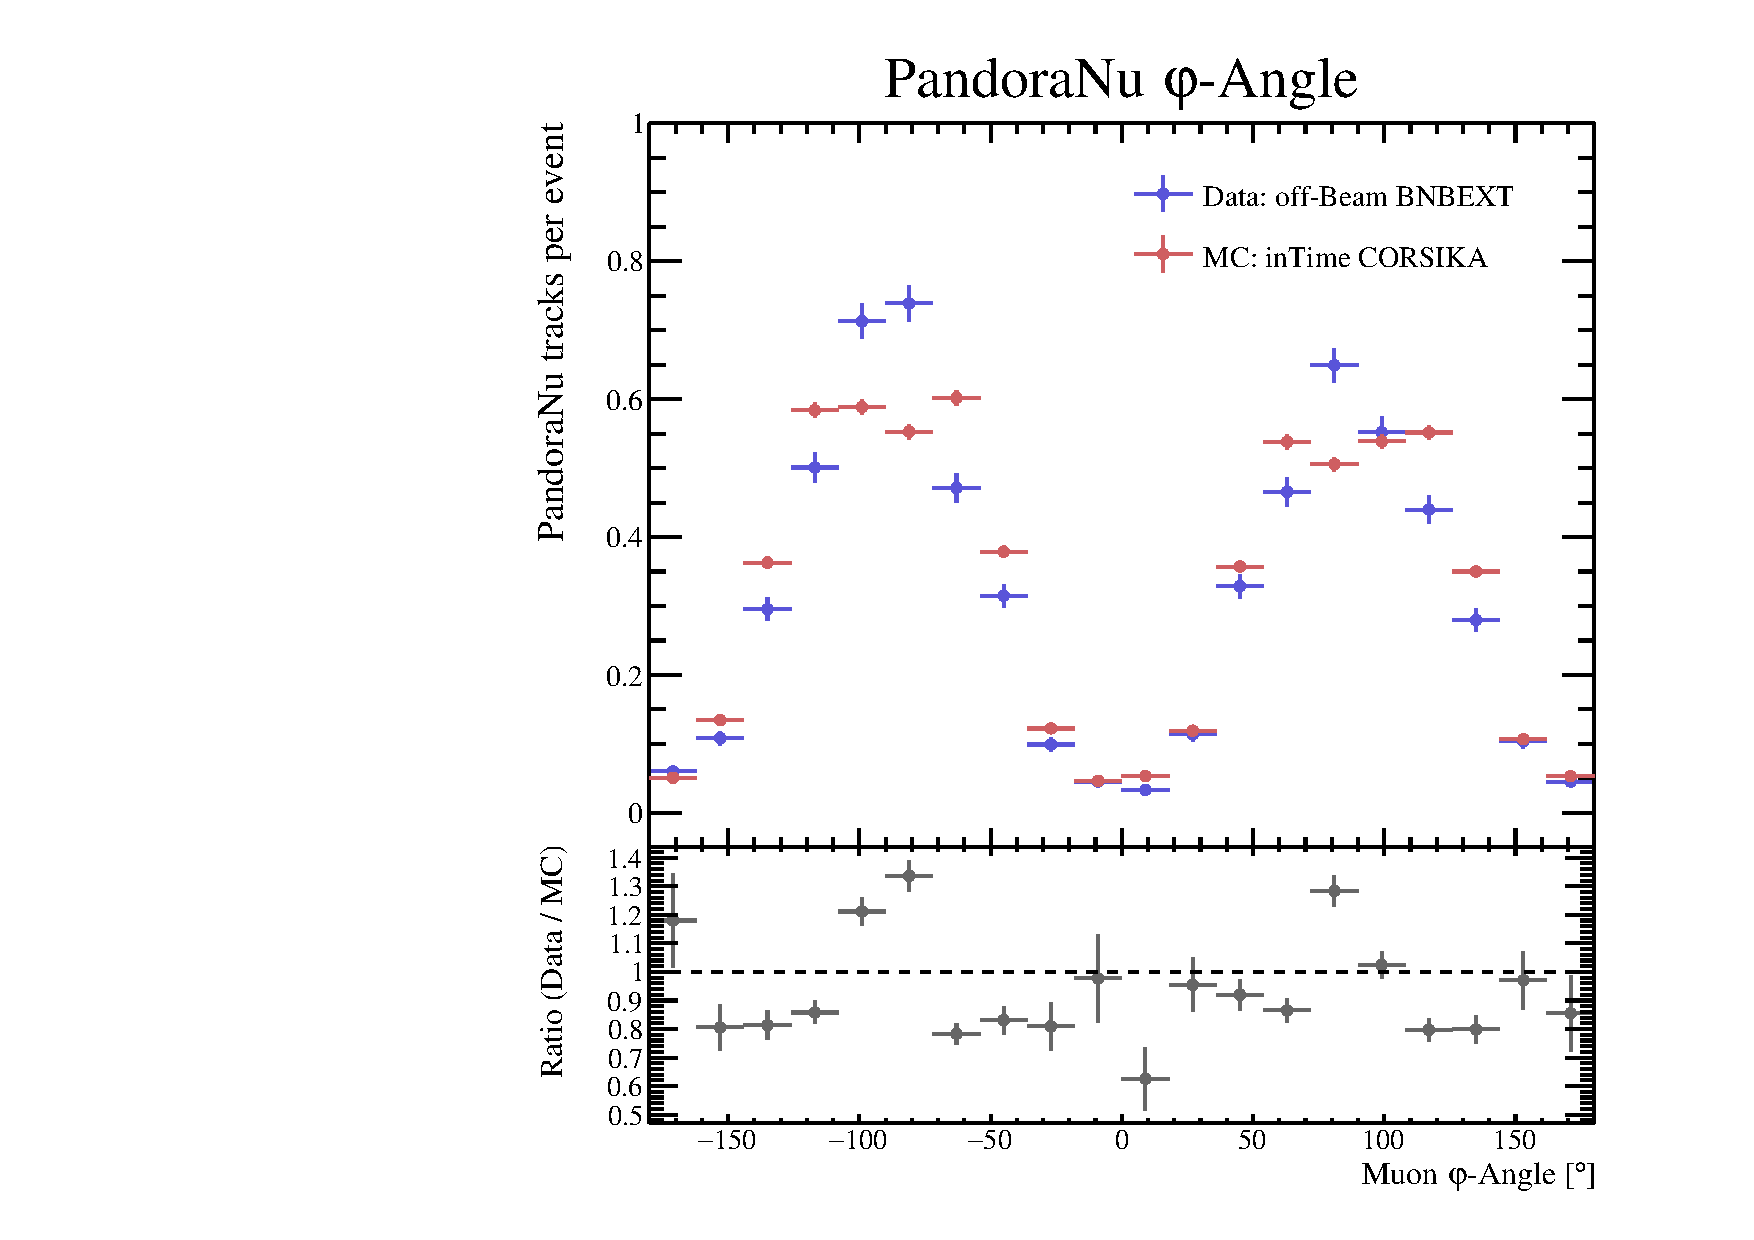
\includegraphics[width=0.5\textwidth]{images/FirstCCInclusive/CosmicBackground/CosmicPhiPandoraNu.pdf}
        \label{fig:PhiPandoraNu}
    }
    \caption[Cosmic-Ray Reconstruction $\phi$-Angle Distributions]{These two graphs depict $\phi$-angle distributions of the inTime cosmic \gls{mc} sample and the off-beam data set. In \subref{fig:PhiPandoraCosmic} the pandoraCosmic pass distributions are shown, while \subref{fig:PhiPandoraNu} depicts the distributions of the pandoraNu pass of the data reconstruction. Note that pandoraCosmic always assumes the tracks as downwards pointing, hence, there is only one peak around $\phi = \SI{-90}{\degree}$.}
    \label{fig:CosmicRecoPhi}
\end{figure}
\begin{figure}[htbp]
    \centering
    \subfloat[][]
    {
        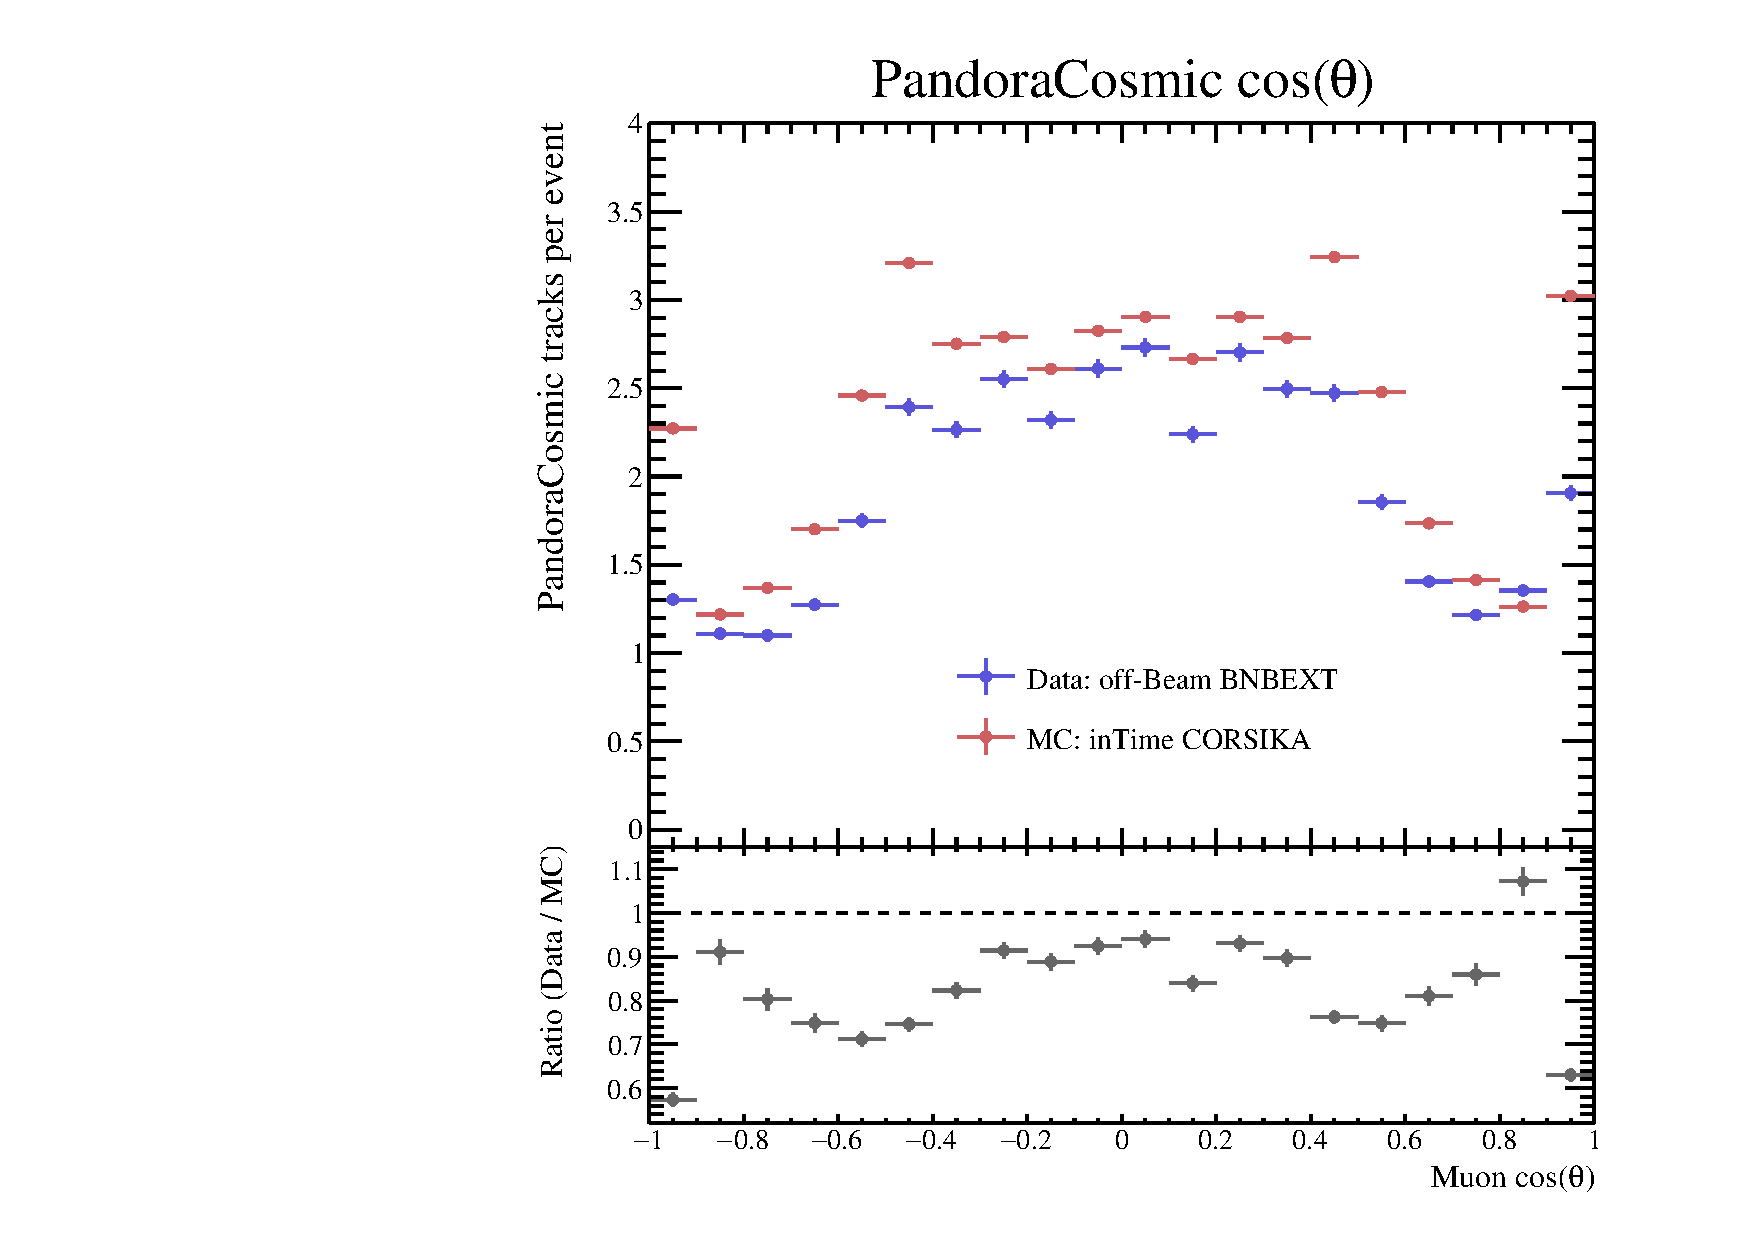
\includegraphics[width=0.5\textwidth]{images/FirstCCInclusive/CosmicBackground/CosmicCosThetaPandoraCosmic.pdf}
        \label{fig:CosThetaPandoraCosmic}
    }
    \subfloat[][]
    {
        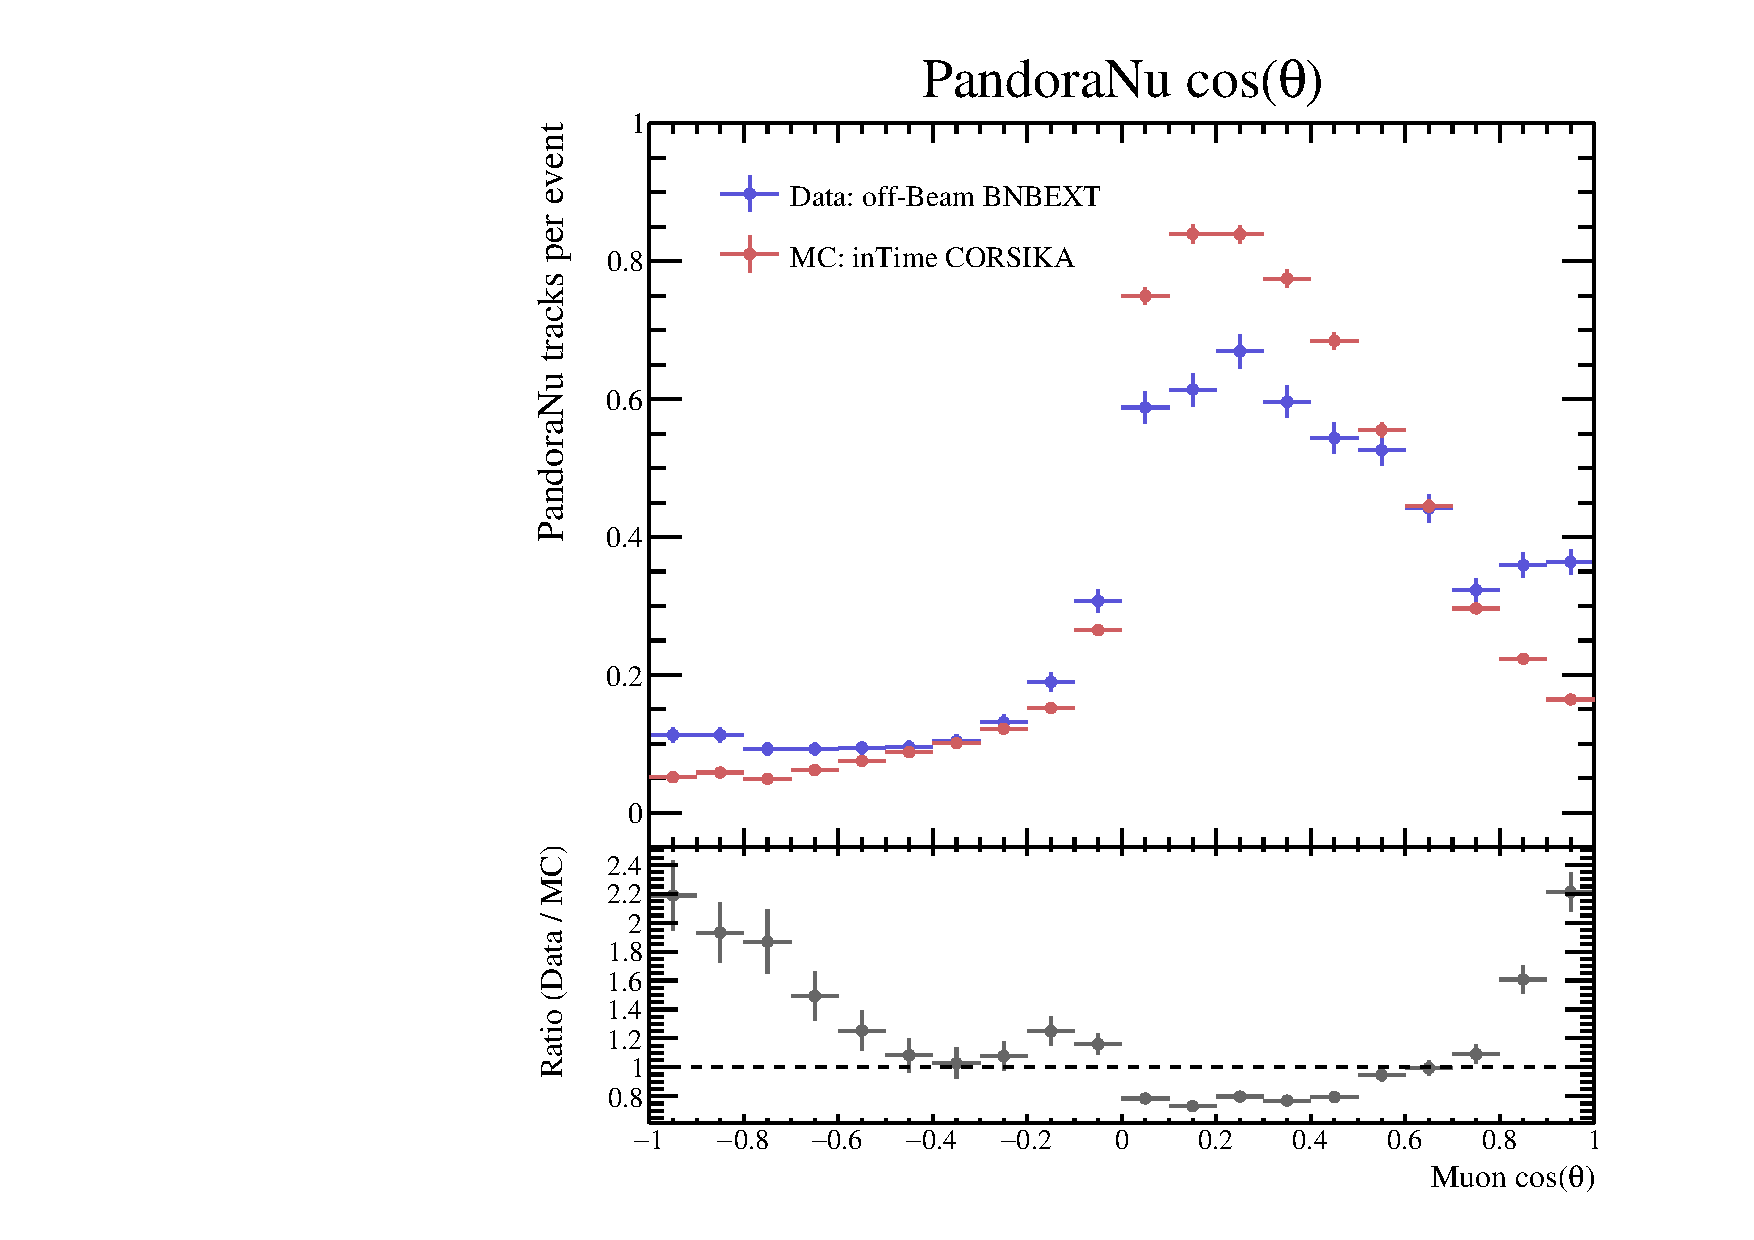
\includegraphics[width=0.5\textwidth]{images/FirstCCInclusive/CosmicBackground/CosmicCosThetaPandoraNu.pdf}
        \label{fig:CosThetaPandoraNu}
    }
    \caption[Cosmic-Ray Reconstruction $\cos{(\theta)}$ Distributions]{These two graphs depict $\cos{(\theta)}$ distributions of the inTime cosmic \gls{mc} sample and the off-beam data set. In \subref{fig:PhiPandoraCosmic} the pandoraCosmic pass distributions are shown, while \subref{fig:PhiPandoraNu} depicts the distributions of the pandoraNu pass of the data reconstruction. Note that pandoraNu prefers to reconstruct tracks as forward pointing, hence, the bias for $\cos{(\theta)} > 0$.}
    \label{fig:CosmicRecoCosTheta}
\end{figure}
Interestingly, when comparing the pandoraNu $\phi$-angle distributions, two peaks of the off-beam sample at around \SI{-90}{\degree} and \SI{90}{\degree} are quite prominent. A very similar effect is seen in the ratio kinematic distribution of $\phi$ in figure \ref{fig:ForwardFoldedPhi}. When comparing the $\cos{(\theta)}$ distributions in figure \ref{fig:CosmicRecoCosTheta}, it can be seen that the off-beam histogram exceeds the inTime histogram at crucial locations around $\cos{(\theta)} \approx \pm 1$. I call this crucial because of the selection process which relies heavily on forwardness, \ie $\abs{\cos{(\theta)}} \approx 1$ (see section \ref{sec:EventSelection}). In these most critical bins, the off-beam pandoraNu reconstructed track count exceeds the inTime \gls{mc} by a factor of two, as is shown in the ratio graph in figure \ref{fig:CosThetaPandoraNu}. Therefore, the relative systematic uncertainty of the \gls{mc} cosmic pileup background is chosen to be \SI{100}{\percent}.

Note, that the above-described discrepancies of the $\phi$-angle and $\cos{(\theta)}$ distributions in the pandoraNu reconstruction pass were also seen by a MicroBooNE study with larger sample size. The authors of said study concluded, that the distributions: \cite[\textit{generally show very good agreement between data and MC simulation}]{MicroBooNECosmicMCPN}. Personally, I strongly disagree with this statement, because the discrepancies, although small and localised, are inconveniently located in selection critical bins. Moreover, in regard of the ratios and their uncertainties shown in figures \ref{fig:CosmicRecoPhi} and \ref{fig:CosmicRecoCosTheta}, the claim of a ``\textit{very good agreement}'' seems far fetched. Such problems with simulated cosmic events later prompted the MicroBooNE collaboration to use measurement based cosmic-ray overlays for the \gls{bnb} \gls{mc} samples, instead of relying on cosmic generators and the \gls{LArSoft} detector simulation chain.

Other systematic uncertainties are introduced by the neutrino flux predictions, which are fed into \gls{genie}. Said systematic uncertainties and their origin is already discussed in detail in section \ref{sec:BNB}. The uncertainties of the integrated flux are listed in table \ref{tab:BNBFluxComposition} and the energy dependent flux uncertainties are depicted in figure \ref{fig:BNBFlux}. Moreover, they are also discussed in \cite{BNBBeamFlux,BNBBeamUncertainty}. Since the event yield, \ie the bin entries of the kinematic distribution, and the flux are in a linear relation, the relative uncertainties of the flux are directly applicable to the yield. Therefore, the uncertainty of every selected \gls{mc} event is determined based on the true neutrino energy and flavour using the beam uncertainty information. These are then individually added up for every bin, thus creating a weighted average of a bin's flux systematic uncertainty. This is done for every \gls{mc} related signal and background category. However, there is one exception: the dirt background is hard to model correctly due to the different materials involved and hence, a relative uncertainty of \SI{100}{\percent} is used. This is in accordance with MicroBooNE's other \gls{cc} inclusive measurements \cite{CRTThomasPhD,MicroBooNEFirstCCInclPublished}.

All the above introduced systematic uncertainties are included in the error bars of the kinematic distributions in section \ref{sec:KinematicDistributions}. There, the systematic variances are simply added to the statistical variances. For the upcoming total flux integrated cross section, the same aforementioned procedures are used to determine the systematic uncertainties. In this case, however, the measurement can be thought of, as having just one bin.

\subsection{Total Flux Integrated Cross Section}
The $\nu_\mu$ \gls{cc} inclusive total flux integrated cross section is defined as follows:
\begin{equation} \label{eq:TotalCrossSection}
    \sigma = \frac{N_\text{BNB}-N_\text{BGR}}{\epsilon \cdot T \cdot \Phi_{\nu_{\mu}}},
\end{equation}
with $N_\text{BNB}$ denoting the number of selected on-beam events, $N_\text{BGR}$ the number of background events (off-beam and simulated), $\epsilon$ the selection efficiency, $T$ the total number of target nucleons, and $\Phi_{\nu_{\mu}}$ the total integrated muon neutrino flux of the \gls{bnb}. At this point, this thesis provides almost all of the numbers used in this equation. The values for $N_\text{BNB}$ and $N_\text{BGR}$ can be found in section \ref{sec:SelectionYields}, but mostly need to be scaled to the appropriate \gls{pot} number. All these numbers, scaled to \num{4.95e19} \gls{pot}, are listed in table \ref{tab:ScaledBackgroundAndSignal}.
\begin{table}[htbp]
    \centering
    \caption[Total Cross Section Selection Variables]{Listed here, are the selection yields, introduced in section \ref{sec:SelectionYields}, scaled to \num{4.95e19} \gls{pot}. Furthermore, the respective statistical and systematic uncertainties are also listed. These values, \ie $N_\text{BNB}$ and $N_\text{BGR}$, are used to calculate the total cross section.}
    \begin{tabu}{llrrr}
        \toprule
        \rowfont[c]{\bf}Symbol & Description & Amount & Stat. & Syst. \\
        \midrule
        $N_\text{BNB}$ & \textbf{Selected on-beam events} & \num{3213} & $\pm \num{56.7}$ & \\
        \midrule
        $N_\text{EXT}$ & Cosmic \gls{BeamGate} (off-beam) & \num{1328.4} & $\pm \num{40.4}$ & \\
        $N_\text{Cosmic}$ & Cosmic pileup event & \num{148.1} & $\pm \num{5.65}$ & $\pm \num{148.1}$\\
        $N_\text{NC}$ & \gls{nc} events in \gls{fv} & \num{76.4} & $\pm \num{4.06}$ & $\pm \num{6.98}$ \\
        $N_\text{Dirt}$ & Dirt events (out of \gls{tpc}) & \num{23.0} & $\pm \num{2.23}$ & $\pm \num{23.0}$ \\
        $N_\text{outFV}$ & Vertex out of \gls{fv} & \num{19.4} & $\pm \num{2.04}$ & $\pm \num{1.56}$ \\
        $N_{\bar \nu_{\mu}}$ & $\bar \nu_{\mu}$ \gls{cc} events in \gls{fv} & \num{15.7} & $\pm \num{1.84}$ & $\pm \num{1.37}$ \\
        $N_{\nu_e}$ & $\nu_e$ and $\bar \nu_e$ \gls{cc} events in \gls{fv} & \num{3.87} & $\pm \num{0.91}$ & $\pm \num{0.36}$ \\
        \midrule
        $N_\text{BGR}$ & \textbf{Sum of Backgrounds} & \num{1614.9} & $\pm \num{41.1}$ & $\pm \num{150.0}$ \\
        \bottomrule
        \label{tab:ScaledBackgroundAndSignal}
     \end{tabu}
\end{table}
The integrated $\nu_\mu$ flux can be derived from table \ref{tab:BNBFluxComposition} and the selection efficiency was also calculated in section \ref{sec:SelectionYields}. The only variable left to be calculated, is the number of target nucleons, $T$. It can be easily derived using the equation
\begin{equation}
    T = \rho V_\text{fid} N_\text{nuc} \frac{N_A}{A}.
\end{equation}
Here, $\rho$ is the \gls{lar} density (see table \ref{tab:LArProperties}), $V_\text{fid}$ the \gls{fv}, $N_\text{nuc} = 40$ the number of nucleons per atom, $N_A$ the Avogadro constant, and $A$ the atomic mass of argon (see also table \ref{tab:LArProperties}). The result of above equation, alongside with the efficiency and the integrated $\nu_\mu$ flux for \num{4.95e19} \gls{pot}, are listed in table \ref{tab:TotCrossSectionVariables}.
\begin{table}[htbp]
    \centering
    \caption[Total Cross Section Detector Variables]{Below, the detector variables used to determine the total flux integrated cross section are listed.}
    \begin{tabu}{llrl}
        \toprule
        \rowfont[c]{\bf} Variable name & Symbol & Value & Unit \\
        \midrule
        Integrated $\nu_\mu$ flux & $\Phi_{\nu_{\mu}}$ & \num{3.55(45)e10} & \si{\per\centi\metre\squared} \\
        Number of target nucleons & $T$ & \num{3.904e31} & \\
        Selection efficiency & $\epsilon$ & \num{12.34(14)} & \si{\percent}\\
        \bottomrule
        \label{tab:TotCrossSectionVariables}
    \end{tabu}
\end{table}

Using the values in tables \ref{tab:ScaledBackgroundAndSignal} and \ref{tab:TotCrossSectionVariables} and applying them to equation \ref{eq:TotalCrossSection}, leads to a $\nu_\mu$ \gls{cc} inclusive total flux integrated cross section of:
\begin{equation}
    \sigma_{\nu_{\mu}} = ( \num{0.933} \pm 0.045 (\text{stat.}) \pm 0.146 (\text{syst.}) ) \times \SI{e-38}{\centi\metre\squared}.
\end{equation}
Said number is in agreement with the most recent MicroBooNE measurement at $( \num{0.770} \pm 0.005 (\text{stat.}) \pm 0.113 (\text{syst.}) ) \times \SI{e-38}{\centi\metre\squared}$ \cite{CRTThomasPhD}.

\subsection{Event Views} \label{sec:EventViews}
In this section, some event views of selected $\nu_{\mu}$ \gls{cc} candidate events from the on-beam data stream are presented. Figures \ref{fig:sel1_r5326} to \ref{fig:sel1_r5499} show an assortment of events selected in my analysis. The candidate interaction is shown in all three event views, and additionally in a \gls{3d} event display showing the reconstructed pandoraNu tracks. These events were cherry-picked to include examples for various event signatures \cite{MicroBooNECCInclPN}.

\begin{figure}[htbp]
\begin{adjustwidth}{-1cm}{-1cm}
\centering
\subfloat[][Collection plane (Y)]
   {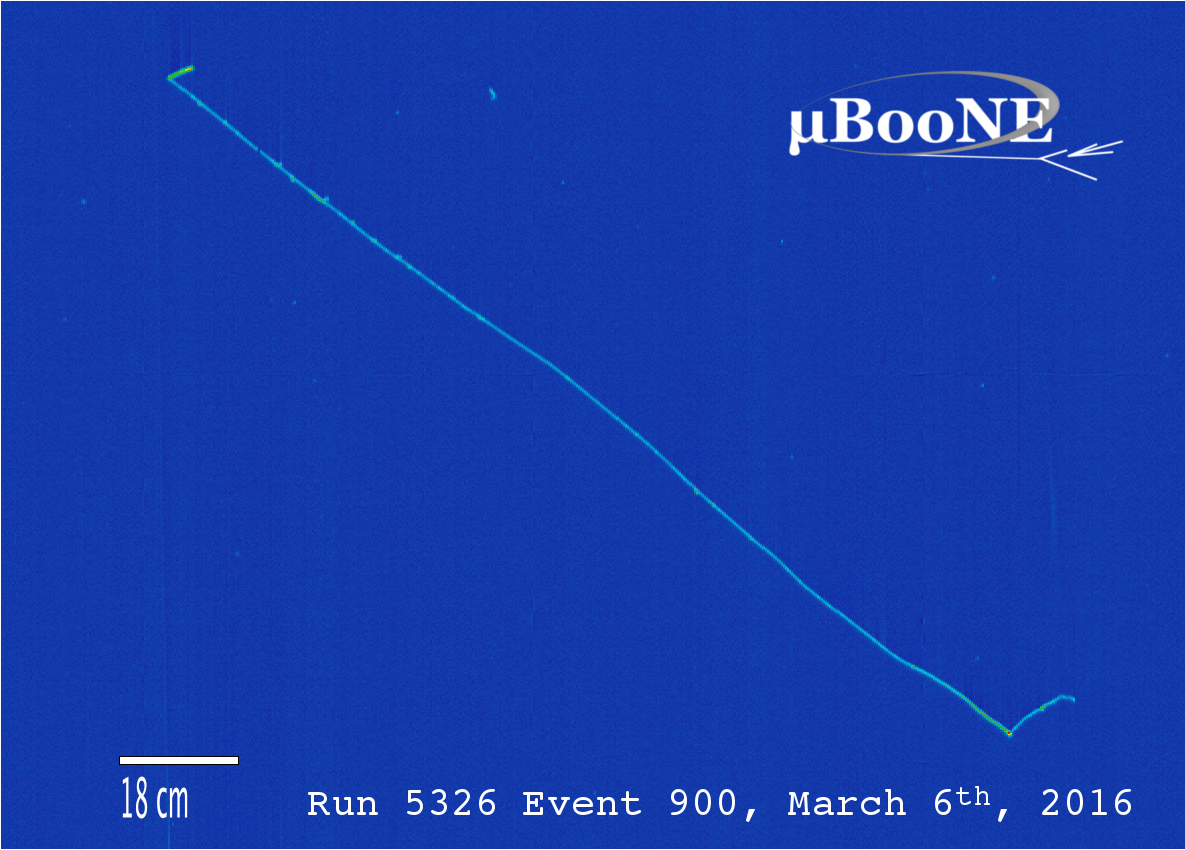
\includegraphics[width=0.5\textwidth + 1cm]{images/FirstCCInclusive/r5326_s17_ev900/plane2.png}
   \label{fig:sel1_r5326_2}}
\subfloat[][Reconstructed 3D image (Y plane projection)]
   {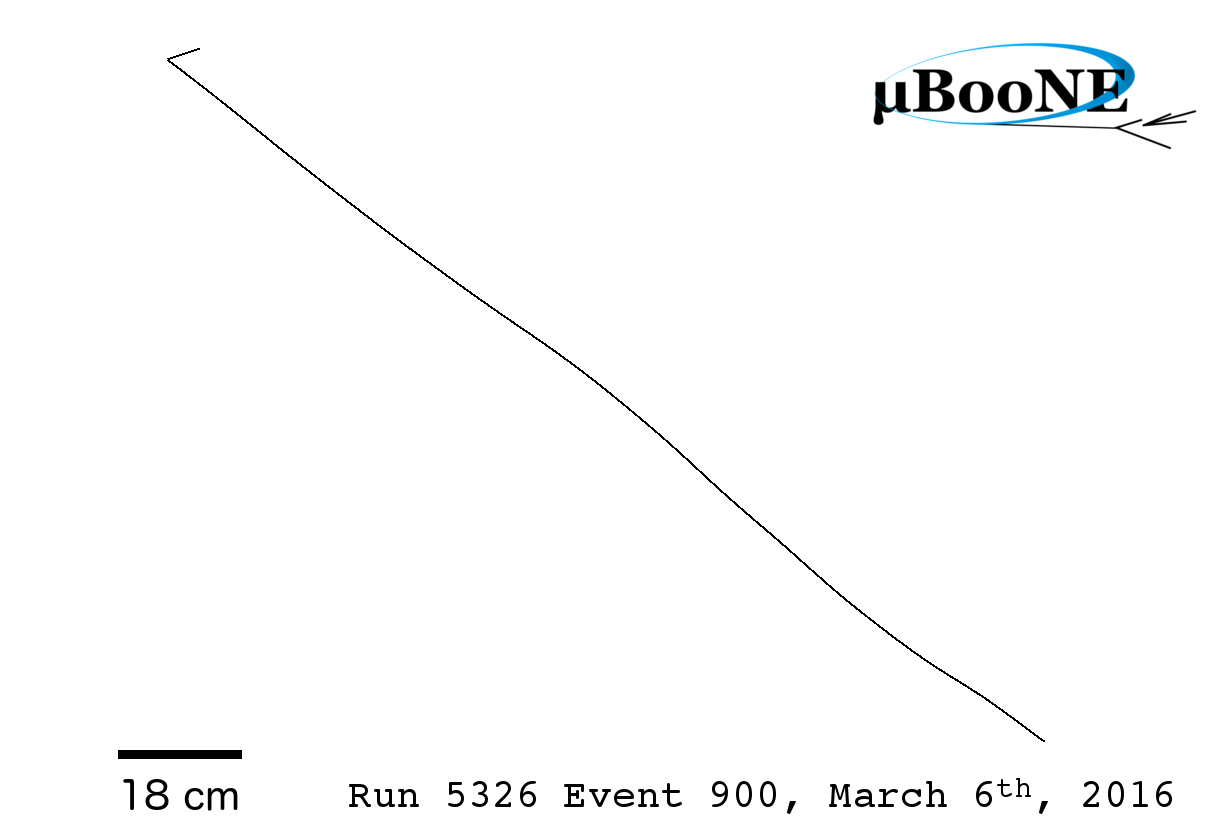
\includegraphics[width=0.5\textwidth + 1cm]{images/FirstCCInclusive/r5326_s17_ev900/plane2_reco.png}
   \label{fig:sel1_r5326_2_reco}} \\
   
\subfloat[][Induction plane (U)]
   {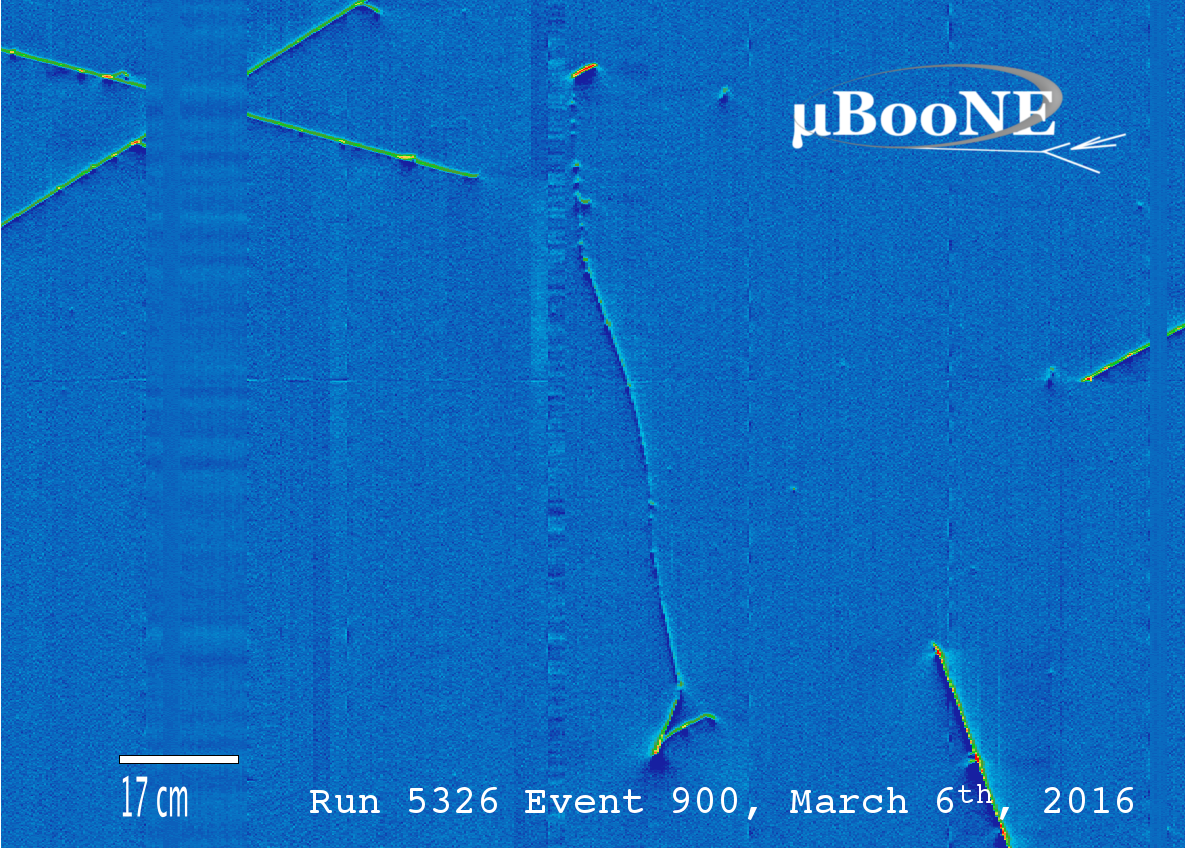
\includegraphics[width=0.5\textwidth + 1cm]{images/FirstCCInclusive/r5326_s17_ev900/plane0.png}
   \label{fig:sel1_r5326_0}} 
\subfloat[][Reconstructed 3D image (U plane projection)]
   {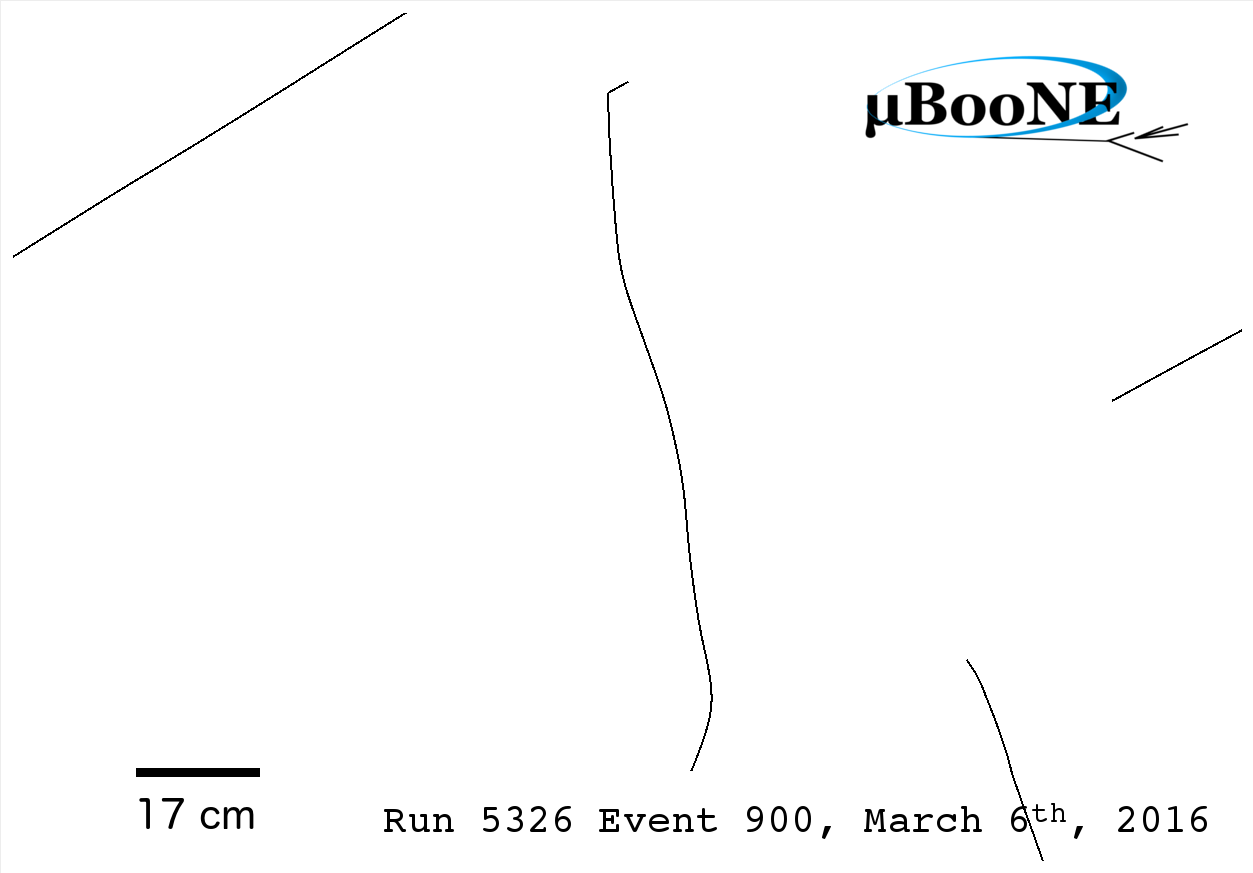
\includegraphics[width=0.5\textwidth + 1cm]{images/FirstCCInclusive/r5326_s17_ev900/plane0_reco.png}
   \label{fig:sel1_r5326_0_reco}} \\   
   
\subfloat[][Induction plane (V)]
   {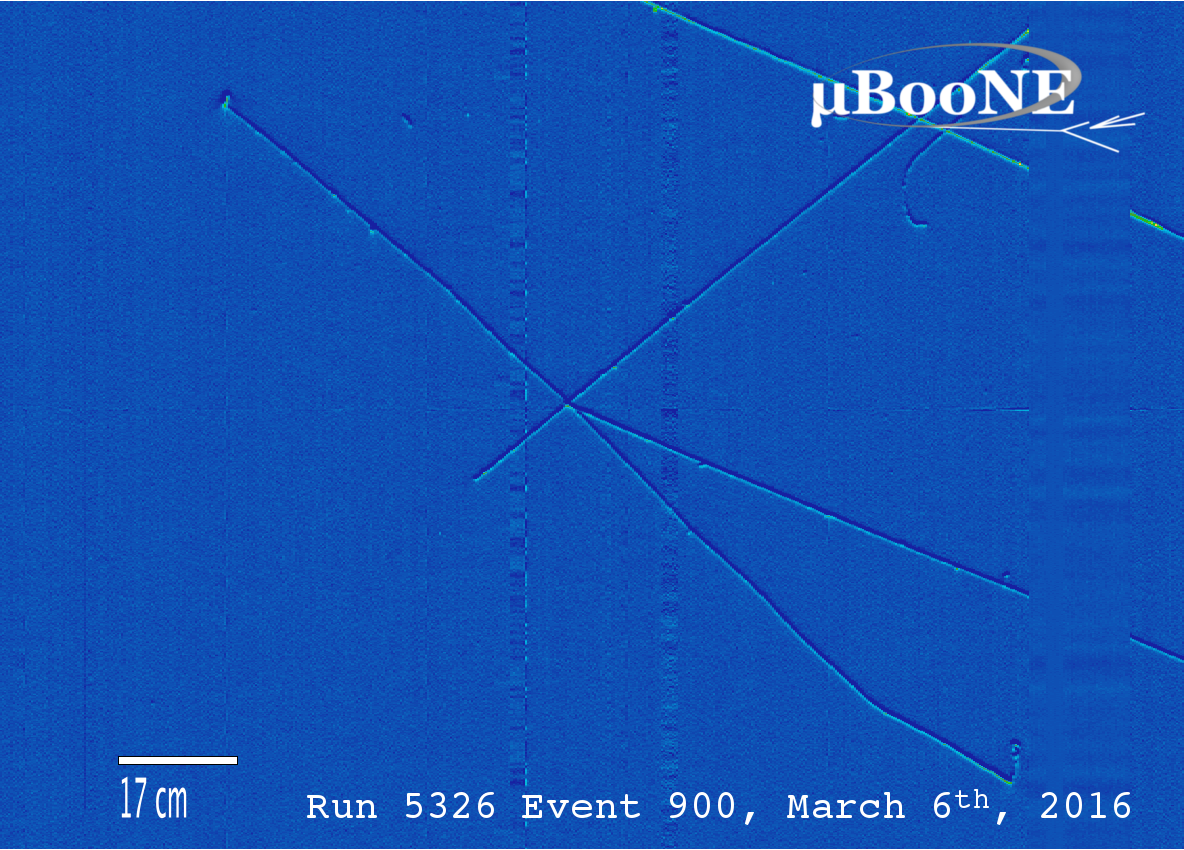
\includegraphics[width=0.5\textwidth + 1cm]{images/FirstCCInclusive/r5326_s17_ev900/plane1.png}
   \label{fig:sel1_r5326_1}} 
\subfloat[][Reconstructed 3D image (V plane projection)]
   {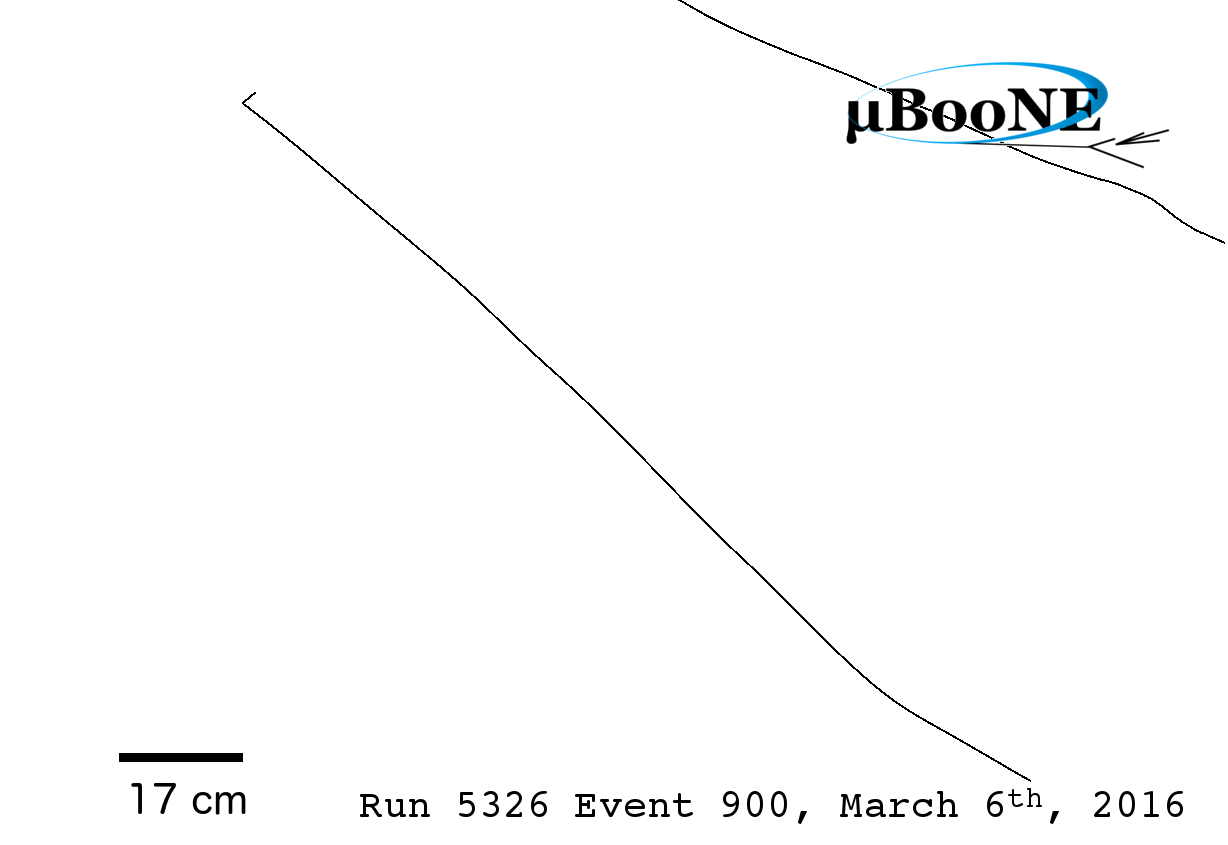
\includegraphics[width=0.5\textwidth + 1cm]{images/FirstCCInclusive/r5326_s17_ev900/plane1_reco.png}
   \label{fig:sel1_r5326_1_reco}} \\  
\caption[Event View for Run 5326, Event 900]{Event view for run 5326, event 900, selected by this analysis. The plots on the left show the event view in all three wire planes. The induction planes show features of gaps of unresponsive wires and noise (see e.g.~left hand side of~\ref{fig:sel1_r5326_1}). The plots on the right show the \gls{3d} reconstructed image projected onto each wire plane. The track reconstruction algorithm shown is pandoraNu. All figures have the same scale (indicated by the bar in the bottom left) and aspect ratio. Sourced from \cite{MicroBooNECCInclPN}.}
\label{fig:sel1_r5326}
\end{adjustwidth}
\end{figure}

\begin{figure}[htbp]
\begin{adjustwidth}{-1cm}{-1cm}
\centering
\subfloat[][Collection plane (Y)]
   {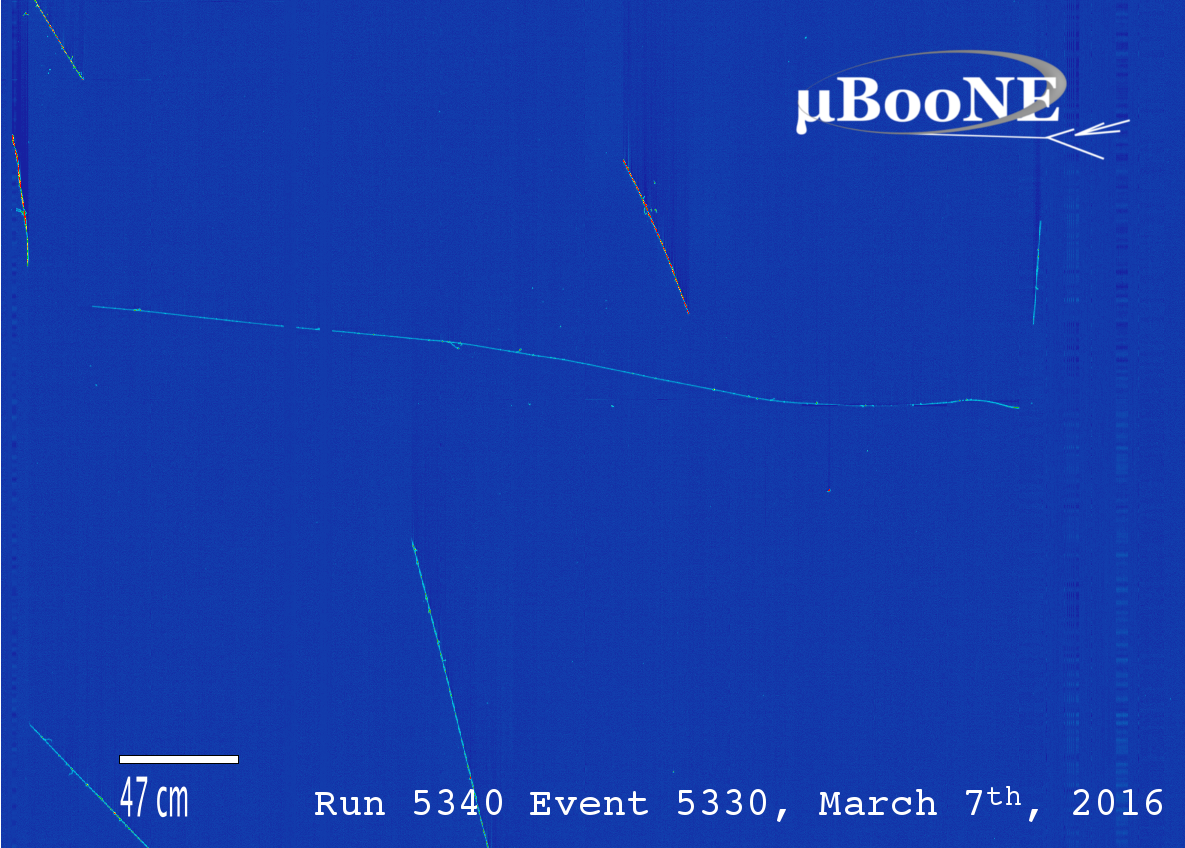
\includegraphics[width=0.5\textwidth + 1cm]{images/FirstCCInclusive/r5340_s106_ev5330/plane2.png}
   \label{fig:sel1_r5340_2}}
\subfloat[][Reconstructed 3D image (Y plane projection)]
   {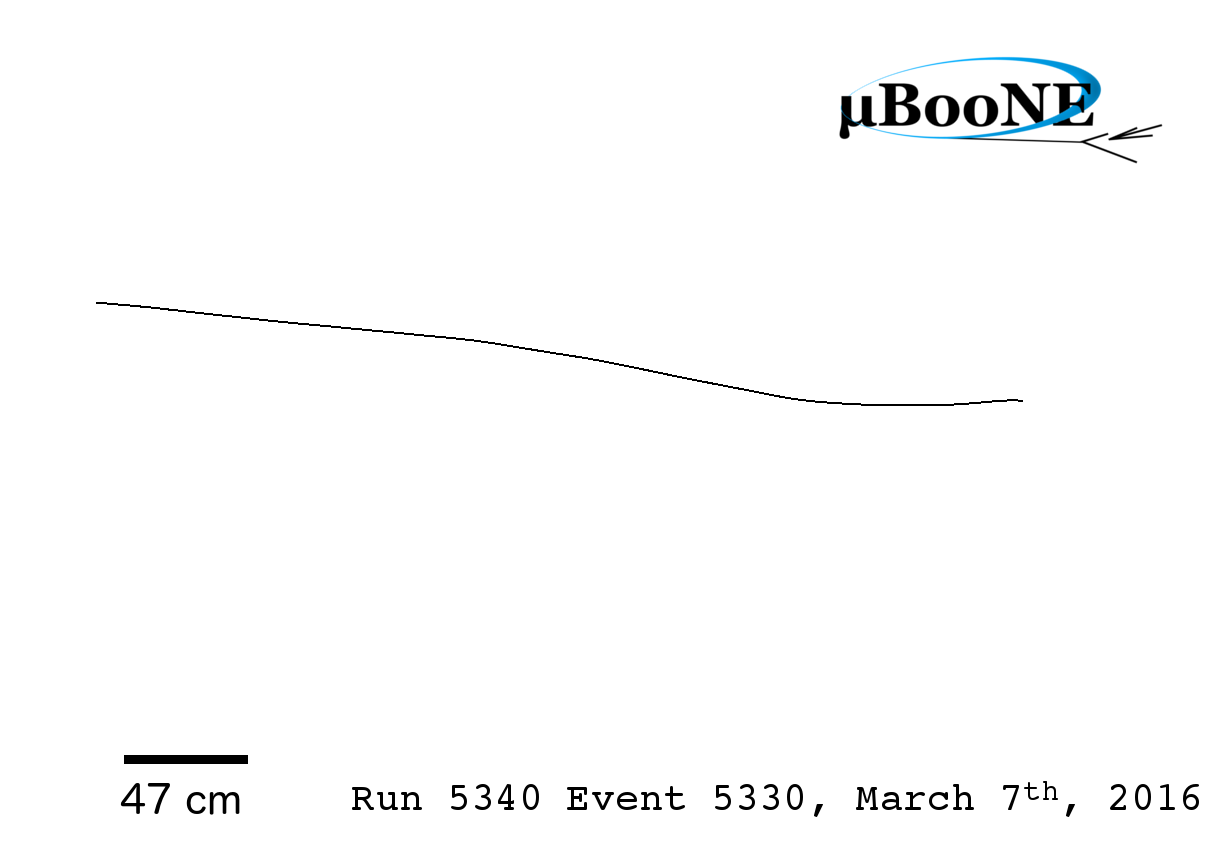
\includegraphics[width=0.5\textwidth + 1cm]{images/FirstCCInclusive/r5340_s106_ev5330/plane2_reco.png}
   \label{fig:sel1_r5340_2_reco}} \\
   
\subfloat[][Induction plane (U)]
   {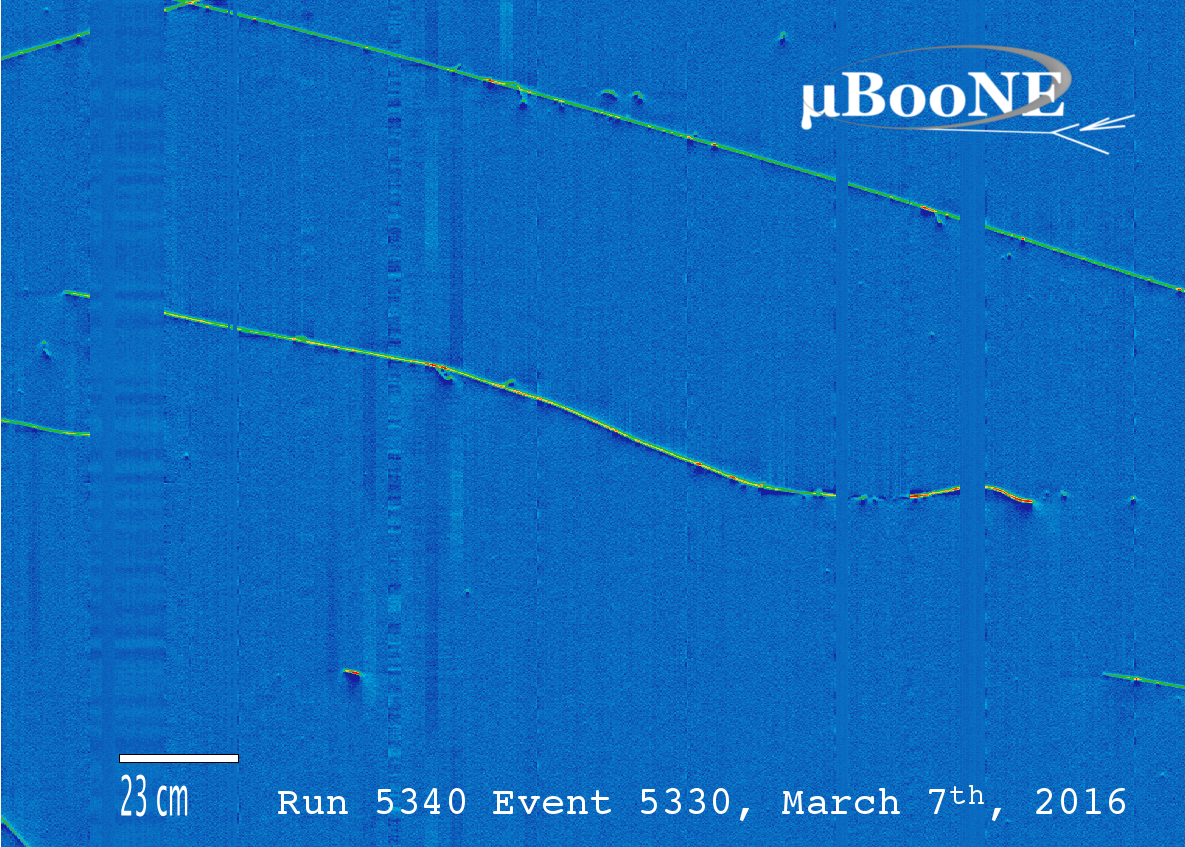
\includegraphics[width=0.5\textwidth + 1cm]{images/FirstCCInclusive/r5340_s106_ev5330/plane0.png}
   \label{fig:sel1_r5340_0}}
\subfloat[][Reconstructed 3D image (U plane projection)]
   {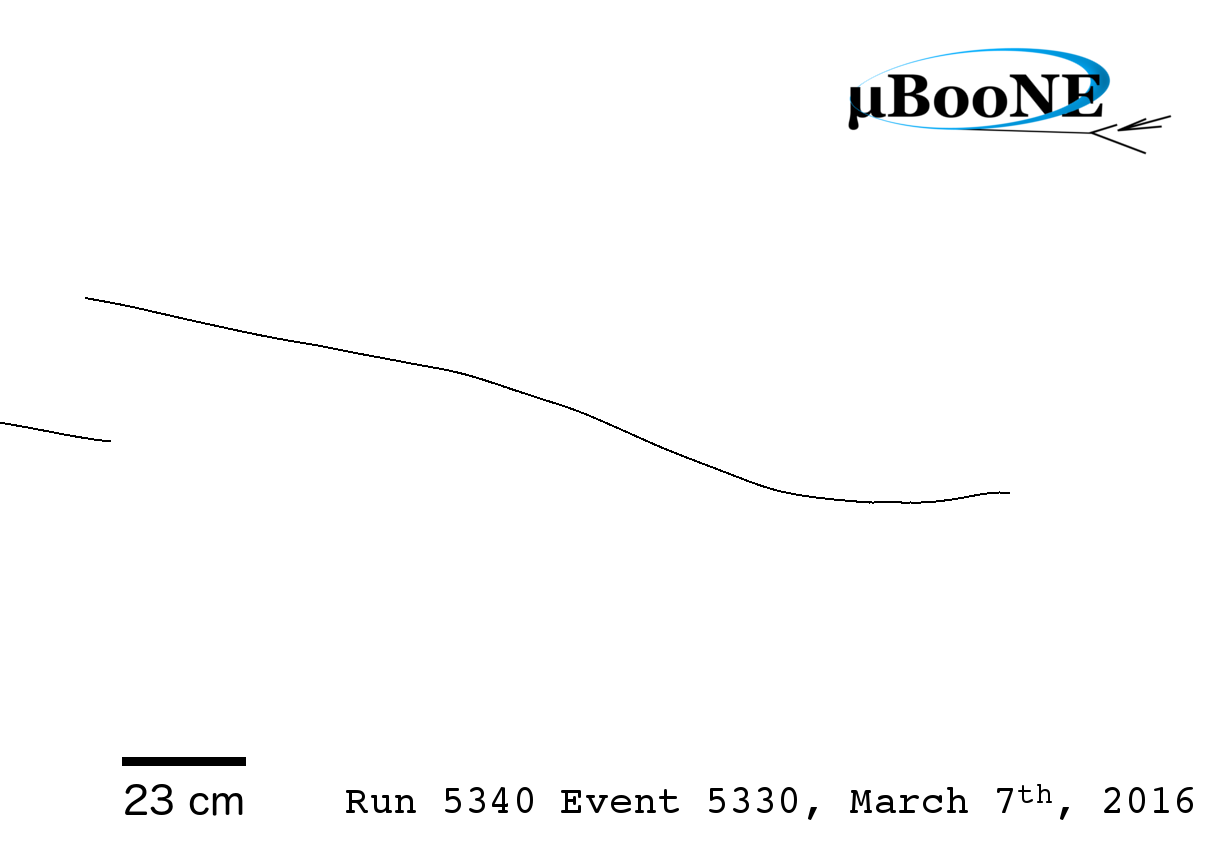
\includegraphics[width=0.5\textwidth + 1cm]{images/FirstCCInclusive/r5340_s106_ev5330/plane0_reco.png}
   \label{fig:sel1_r5340_0_reco}} \\   
   
\subfloat[][Induction plane (V)]
   {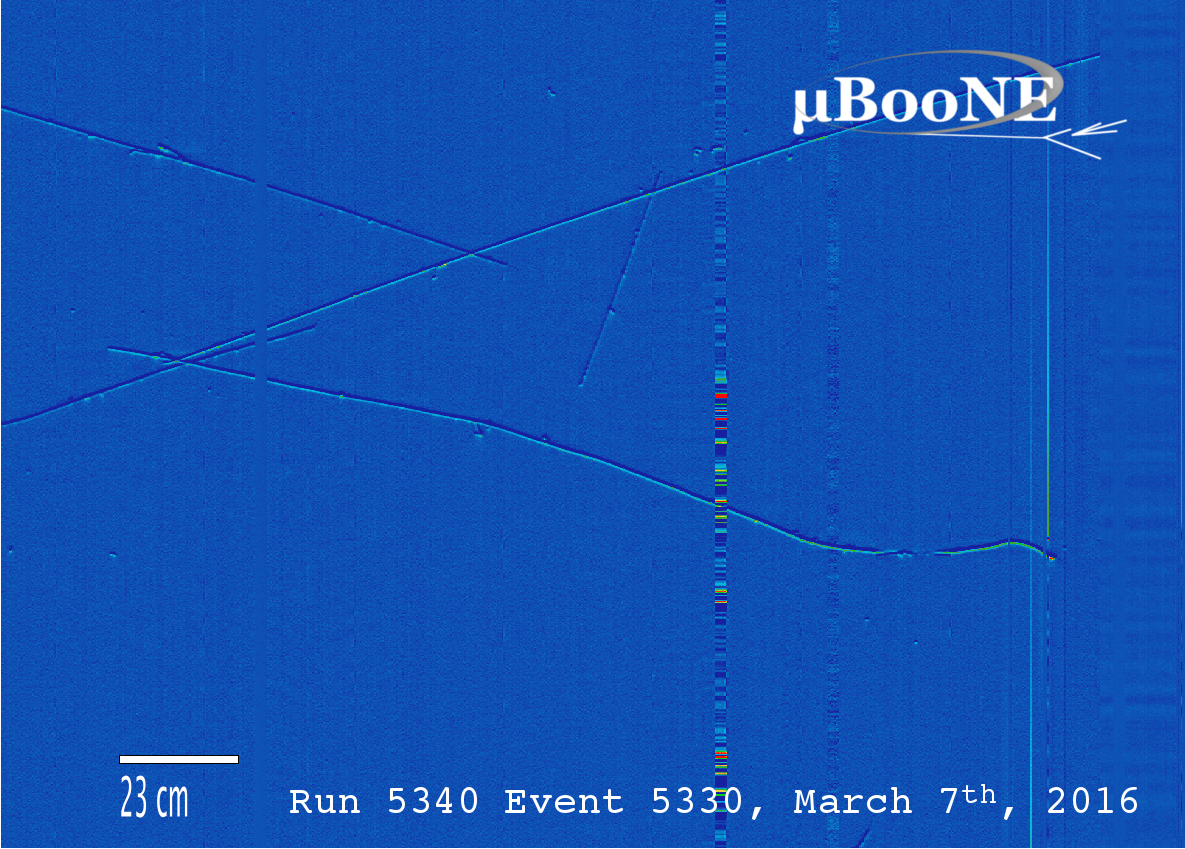
\includegraphics[width=0.5\textwidth + 1cm]{images/FirstCCInclusive/r5340_s106_ev5330/plane1.png}
   \label{fig:sel1_r5340_1}}
\subfloat[][Reconstructed 3D image (V plane projection)]
   {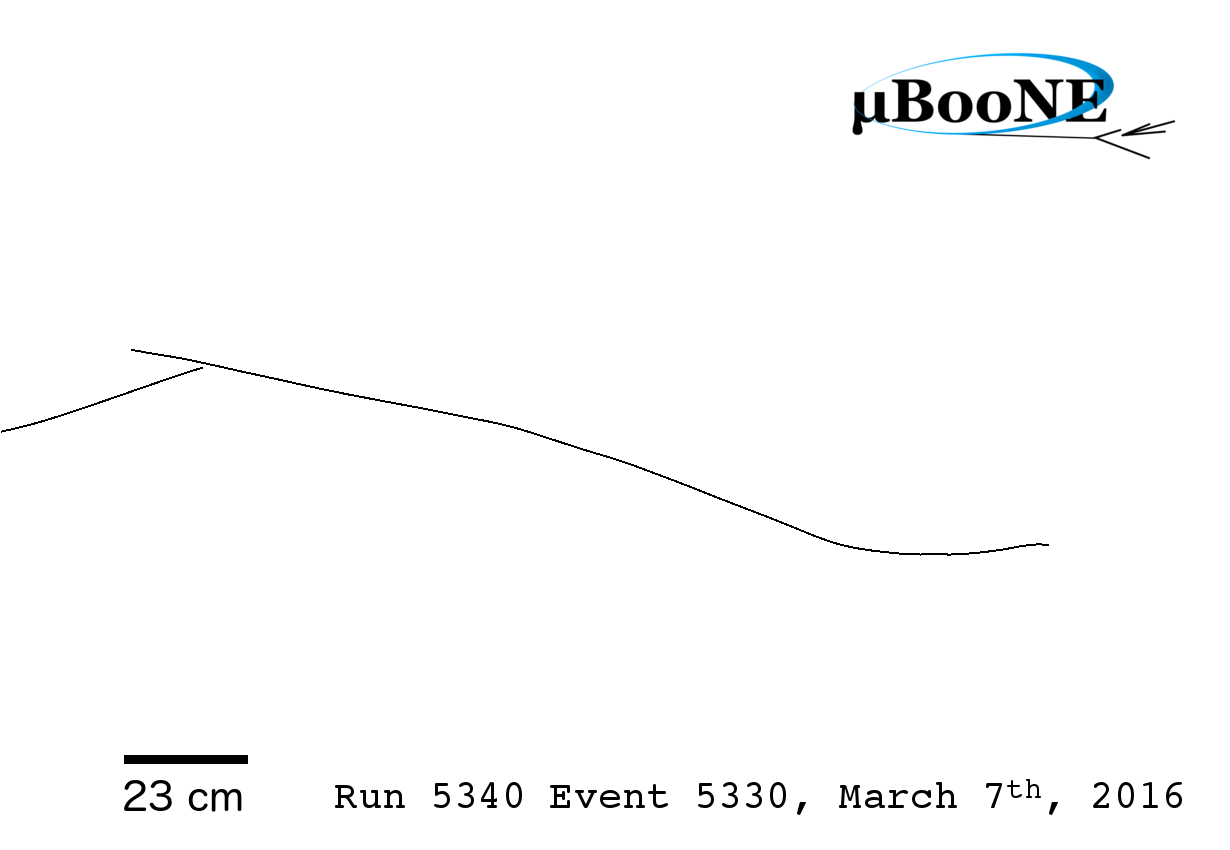
\includegraphics[width=0.5\textwidth + 1cm]{images/FirstCCInclusive/r5340_s106_ev5330/plane1_reco.png}
   \label{fig:sel1_r5340_1_reco}} \\   
\caption[Event View for Run 5340, Event 5330]{Event view for run 5340, event 5330 selected by this analysis. The plots on the left show the event view in all three wire planes. Both induction planes show noise (vertical stripes in Figures \ref{fig:sel1_r5340_0} and \ref{fig:sel1_r5340_1}. The plots on the right show the \gls{3d} reconstructed image projected onto each wire plane. The track reconstruction algorithm shown is pandoraNu. Note that some tracks visible on the left hand plots are missing on the right because they have been rejected in the cosmic removal pass. All figures have the same scale (indicated by the bar in the bottom left) and aspect ratio. Sourced from \cite{MicroBooNECCInclPN}.}
\label{fig:sel1_r5340}
\end{adjustwidth}
\end{figure}

\begin{figure}[htbp]
\begin{adjustwidth}{-1cm}{-1cm}
\centering
\subfloat[][Collection plane (Y)]
   {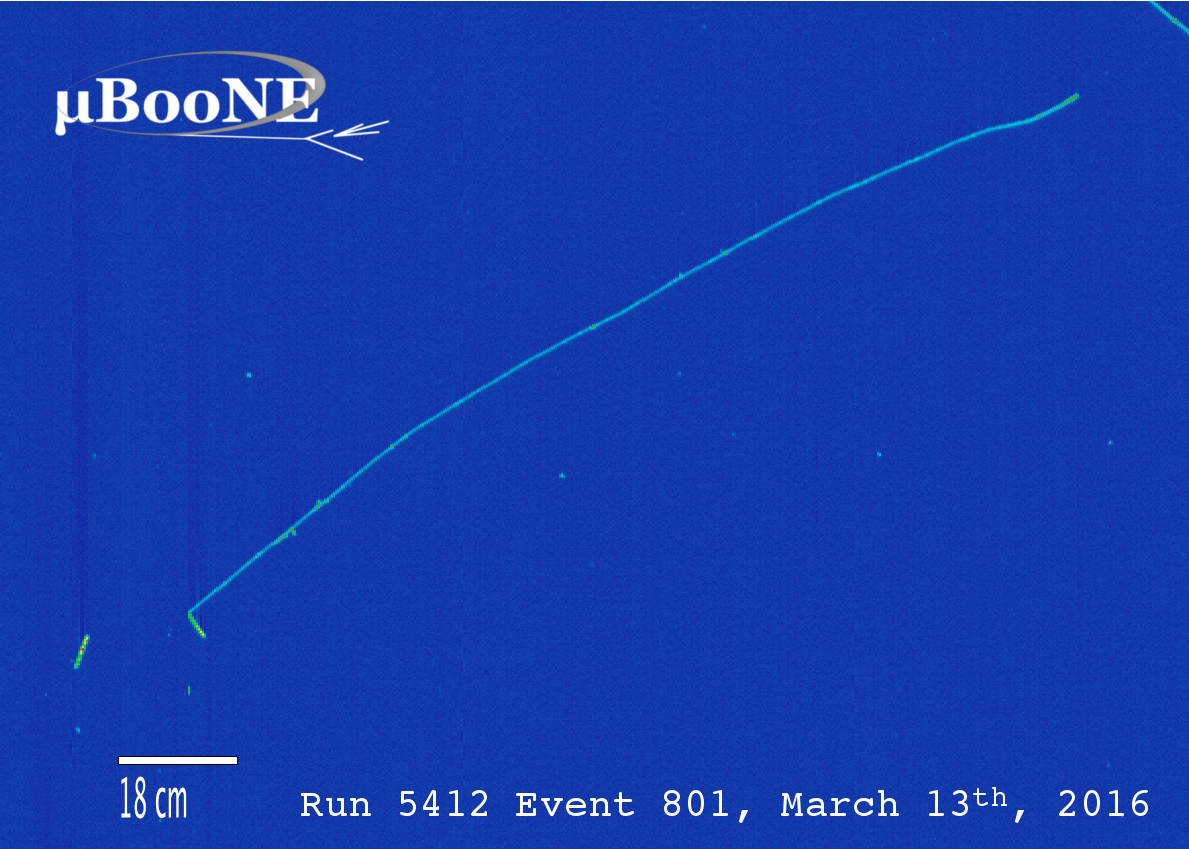
\includegraphics[width=0.5\textwidth + 1cm]{images/FirstCCInclusive/r5412_s16_ev801/plane2.png}
   \label{fig:sel1_r5412_2}}
\subfloat[][Reconstructed 3D image (Y plane projection)]
   {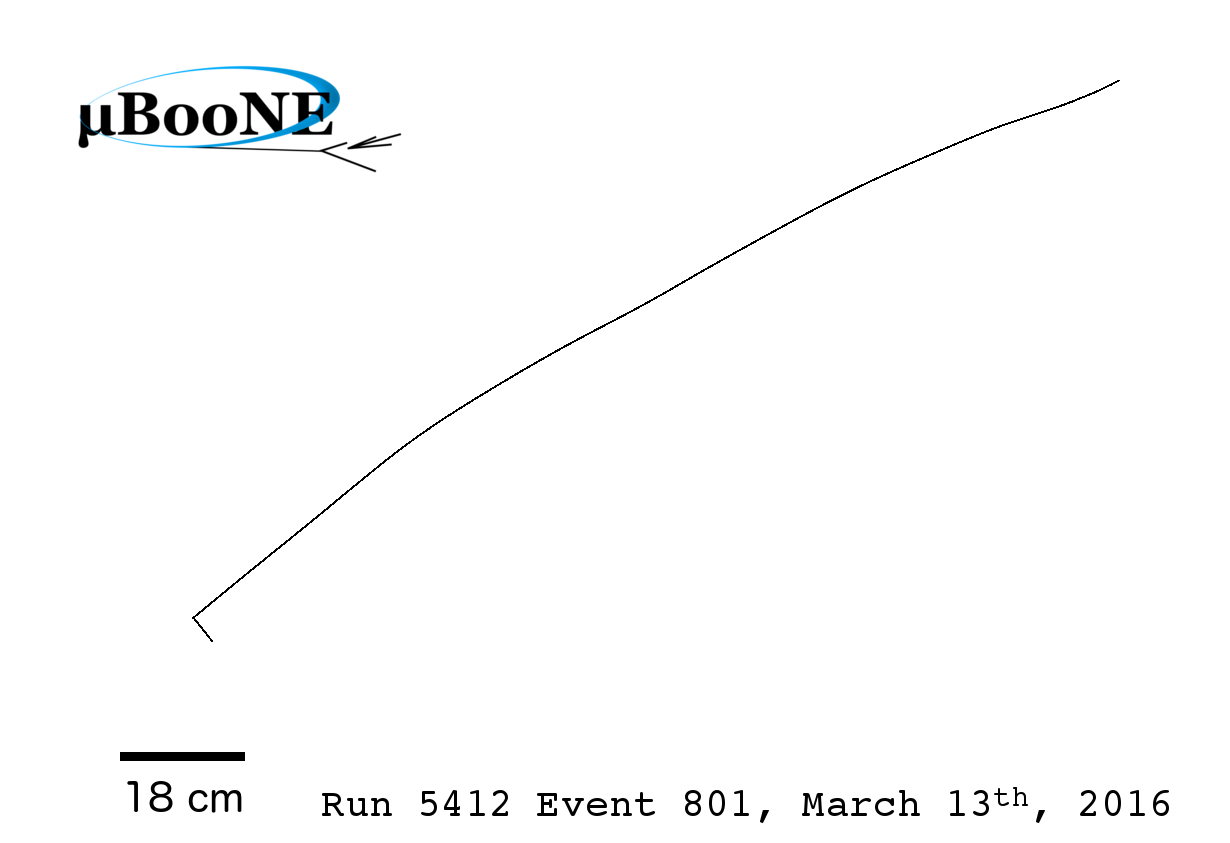
\includegraphics[width=0.5\textwidth + 1cm]{images/FirstCCInclusive/r5412_s16_ev801/plane2_reco.png}
   \label{fig:sel1_r5412_2_reco}} \\
   
\subfloat[][Induction plane (U)]
   {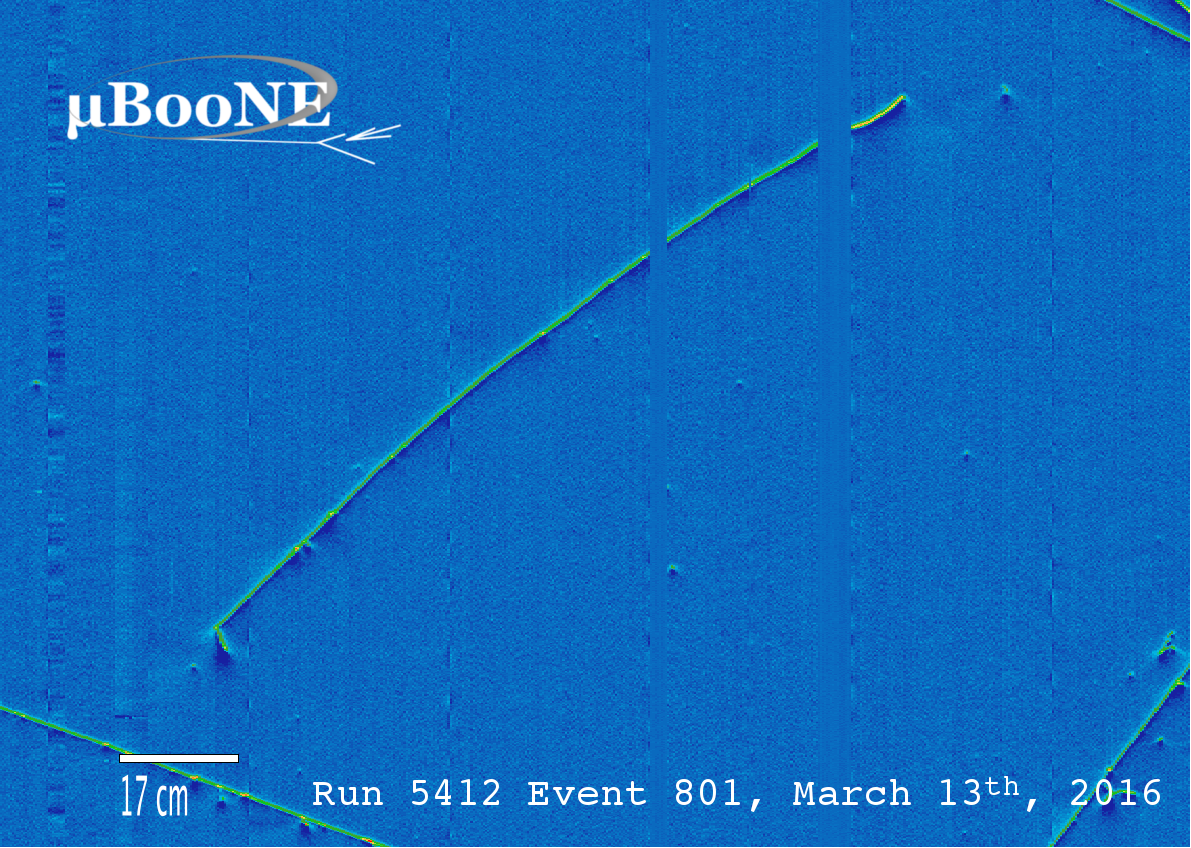
\includegraphics[width=0.5\textwidth + 1cm]{images/FirstCCInclusive/r5412_s16_ev801/plane0.png}
   \label{fig:sel1_r5412_0}}
\subfloat[][Reconstructed 3D image (U plane projection)]
   {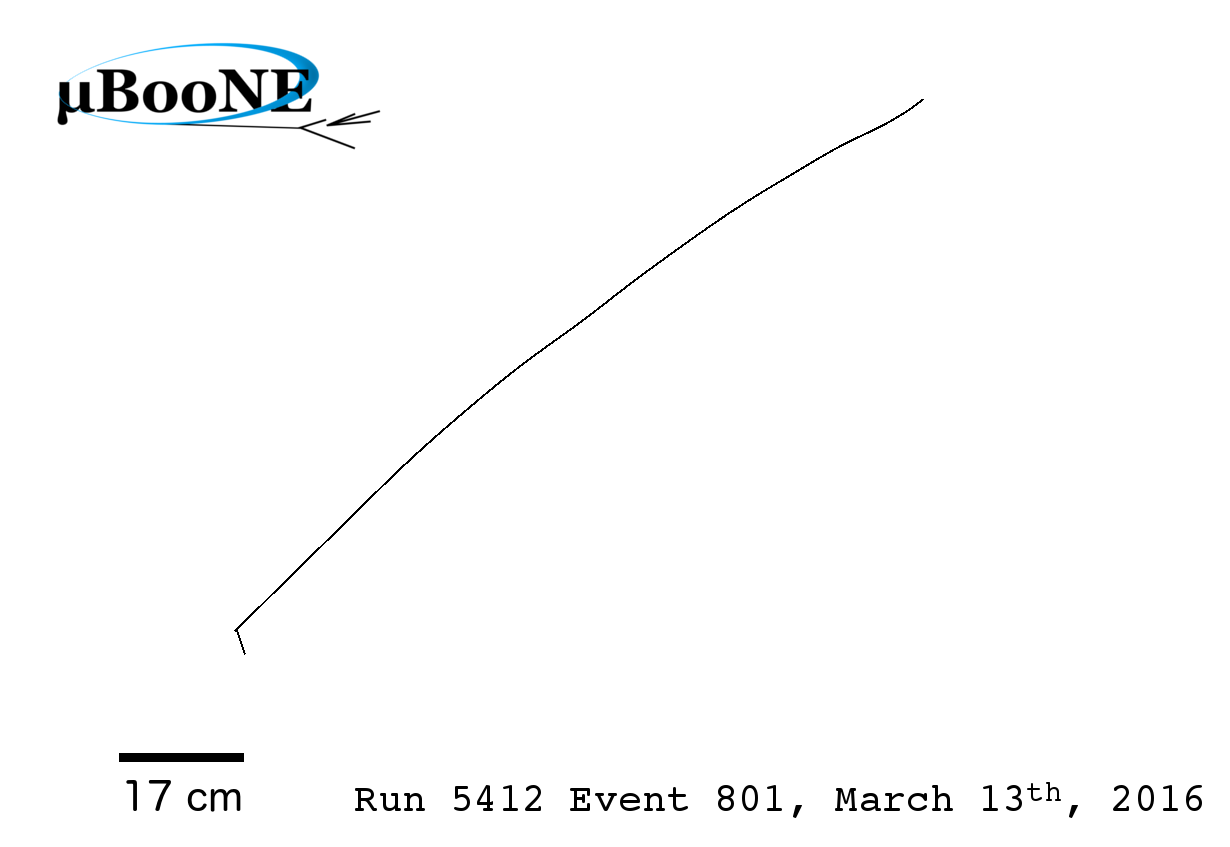
\includegraphics[width=0.5\textwidth + 1cm]{images/FirstCCInclusive/r5412_s16_ev801/plane0_reco.png}
   \label{fig:sel1_r5412_0_reco}} \\   
   
\subfloat[][Induction plane (V)]
   {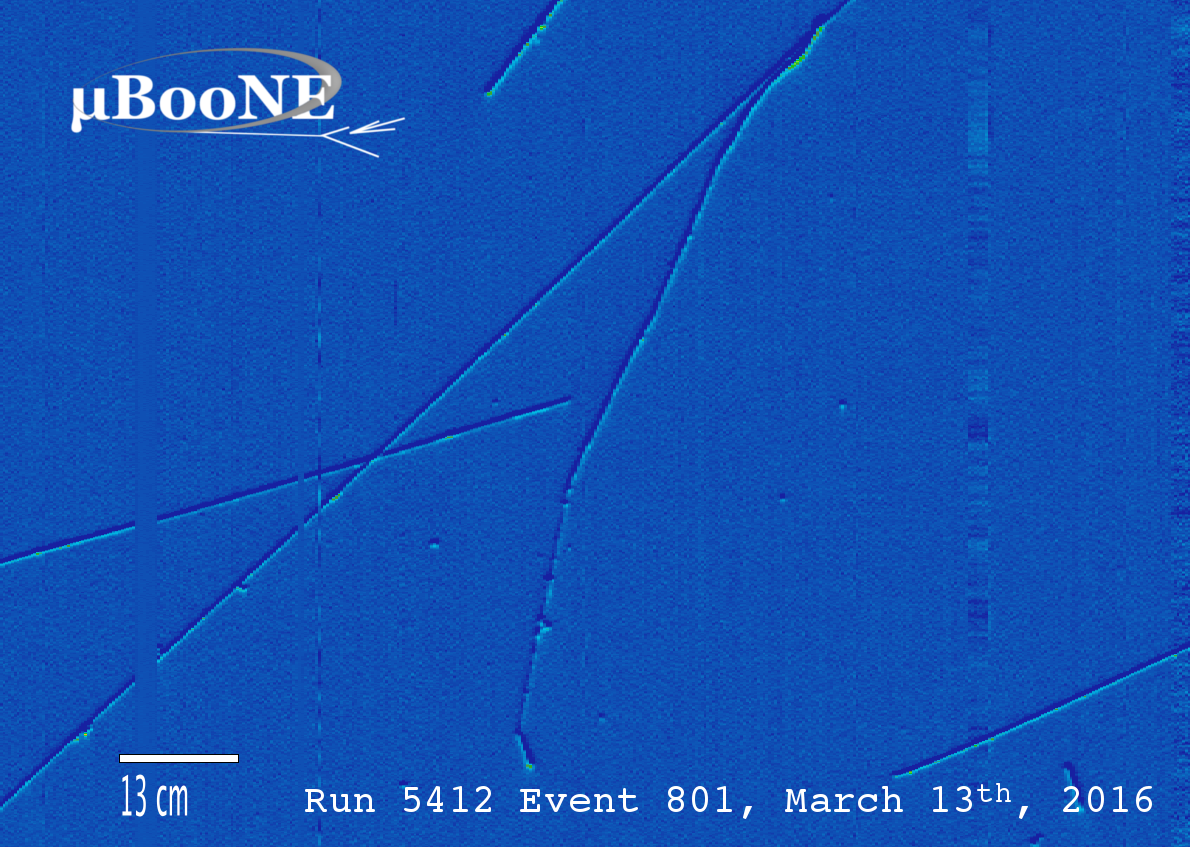
\includegraphics[width=0.5\textwidth + 1cm]{images/FirstCCInclusive/r5412_s16_ev801/plane1.png}
   \label{fig:sel1_r5412_1}}
\subfloat[][Reconstructed 3D image (V plane projection)]
   {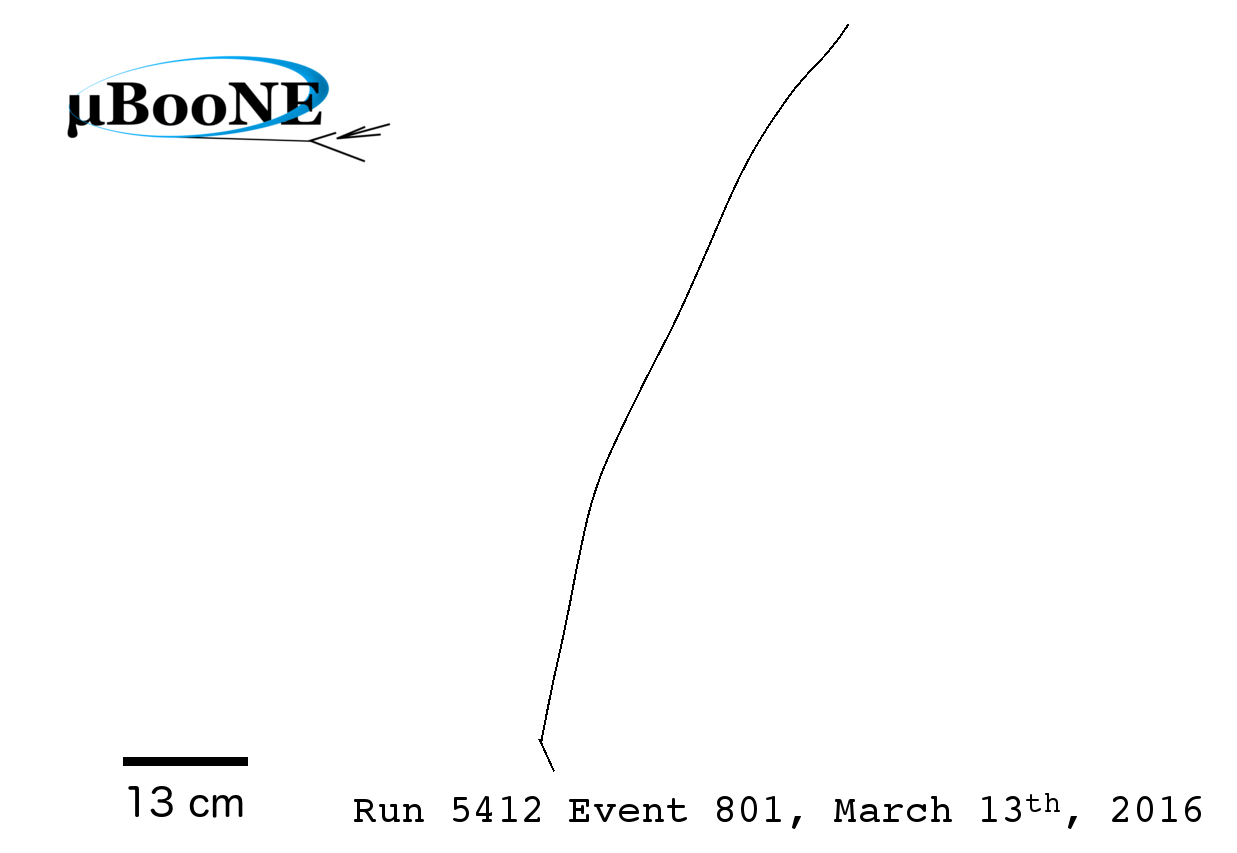
\includegraphics[width=0.5\textwidth + 1cm]{images/FirstCCInclusive/r5412_s16_ev801/plane1_reco.png}
   \label{fig:sel1_r5412_1_reco}} \\   
\caption[Event View for Run 5412, Event 801]{Event view for run 5412, event 801, selected by this analysis. The plots on the left show the event view in all three wire planes. The plots on the right show the \gls{3d} reconstructed image projected onto each wire plane. The track reconstruction algorithm shown is pandoraNu. Note that some tracks visible on the left hand plots are missing on the right because they have been rejected in the cosmic removal pass. All figures have the same scale (indicated by the bar in the bottom left) and aspect ratio. Sourced from \cite{MicroBooNECCInclPN}.}
\label{fig:sel1_r5412}
\end{adjustwidth}
\end{figure}

\begin{figure}[htbp]
\begin{adjustwidth}{-1cm}{-1cm}
\centering
\subfloat[][Collection plane (Y)]
   {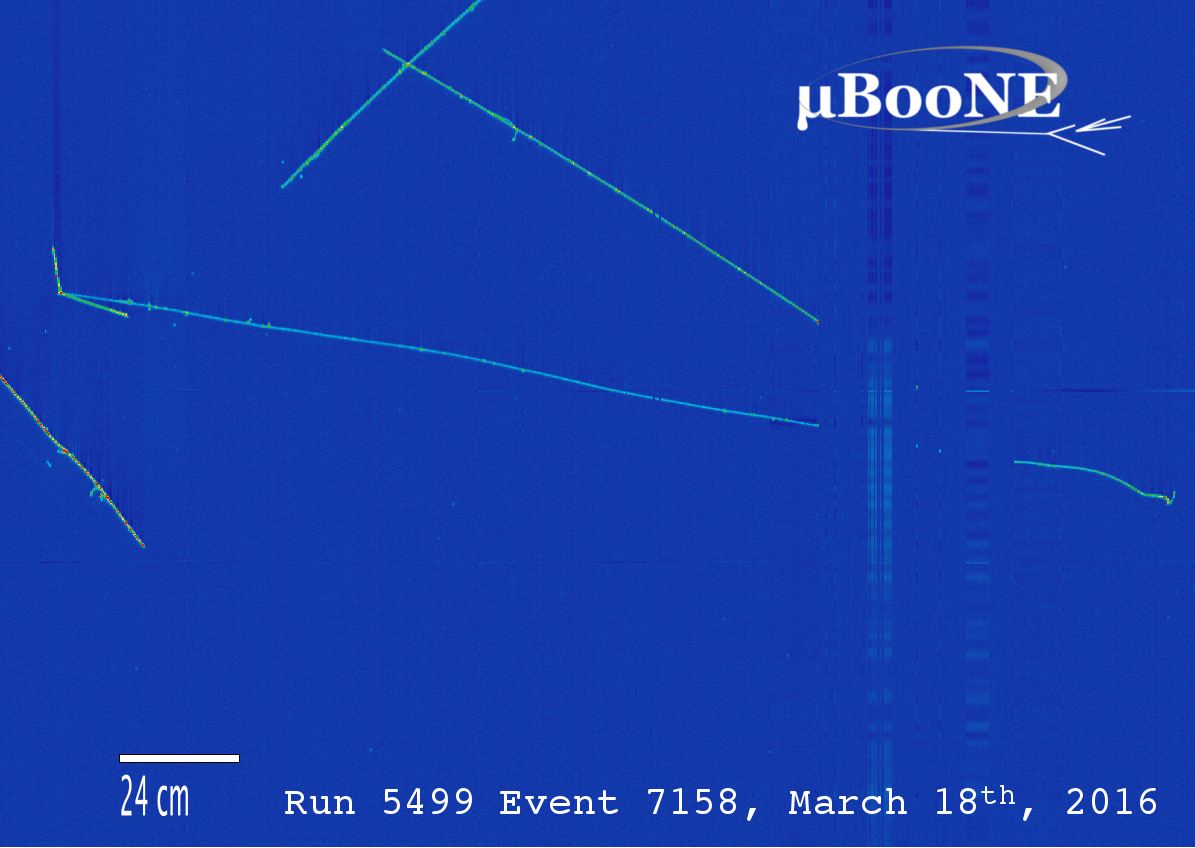
\includegraphics[width=0.5\textwidth + 1cm]{images/FirstCCInclusive/r5499_s143_ev7158/plane2.png}
   \label{fig:sel1_r5499_2}}
\subfloat[][Reconstructed 3D image (Y plane projection)]
   {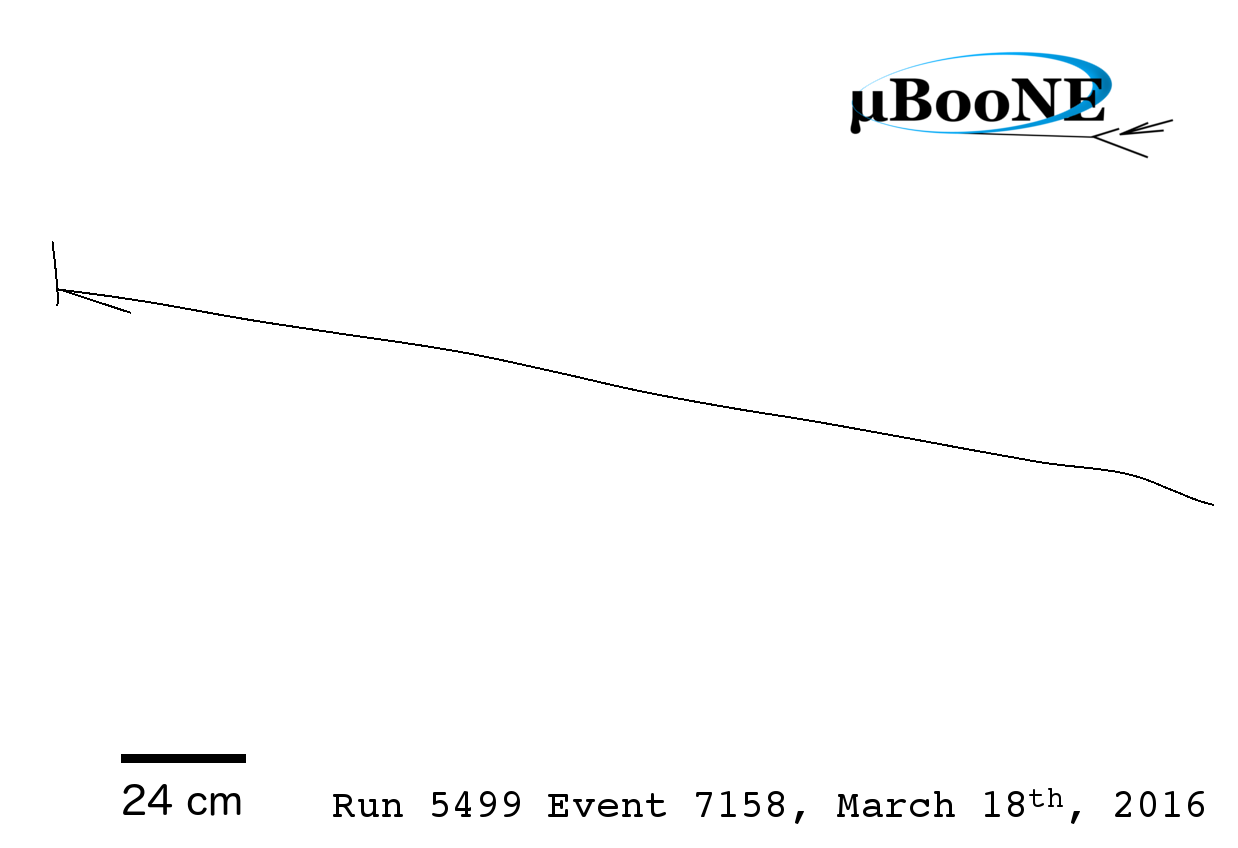
\includegraphics[width=0.5\textwidth + 1cm]{images/FirstCCInclusive/r5499_s143_ev7158/plane2_reco.png}
   \label{fig:sel1_r5499_2_reco}} \\
   
\subfloat[][Induction plane (U)]
   {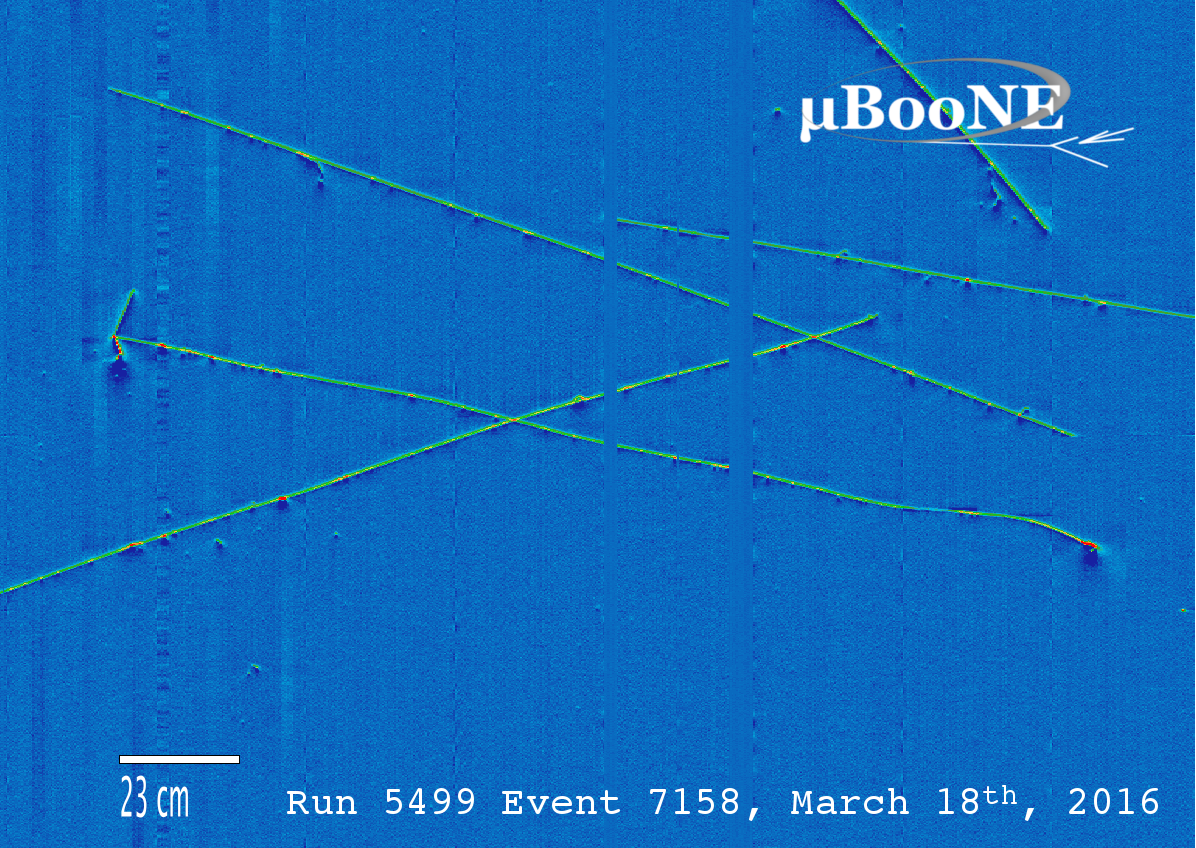
\includegraphics[width=0.5\textwidth + 1cm]{images/FirstCCInclusive/r5499_s143_ev7158/plane0.png}
   \label{fig:sel1_r5499_0}}
\subfloat[][Reconstructed 3D image (U plane projection)]
   {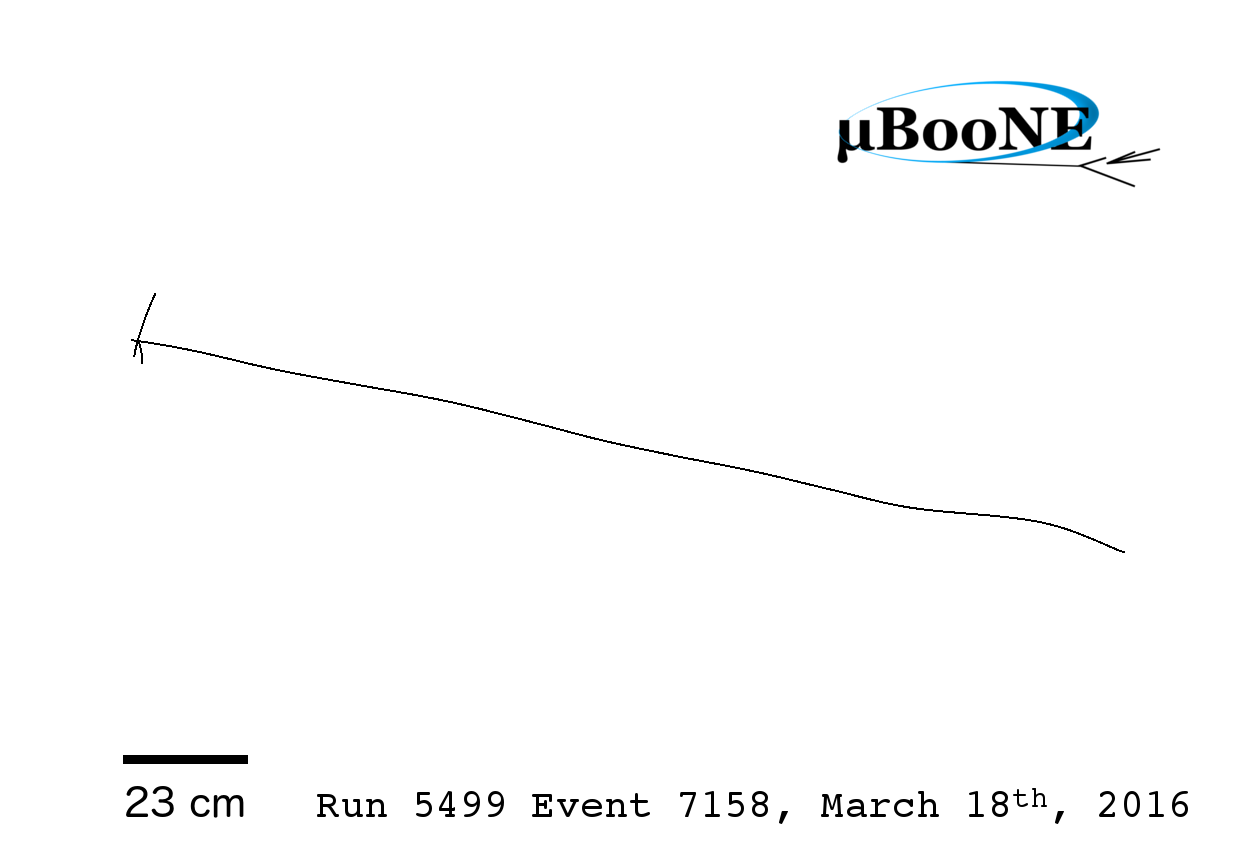
\includegraphics[width=0.5\textwidth + 1cm]{images/FirstCCInclusive/r5499_s143_ev7158/plane0_reco.png}
   \label{fig:sel1_r5499_0_reco}} \\   
   
\subfloat[][Induction plane (V)]
   {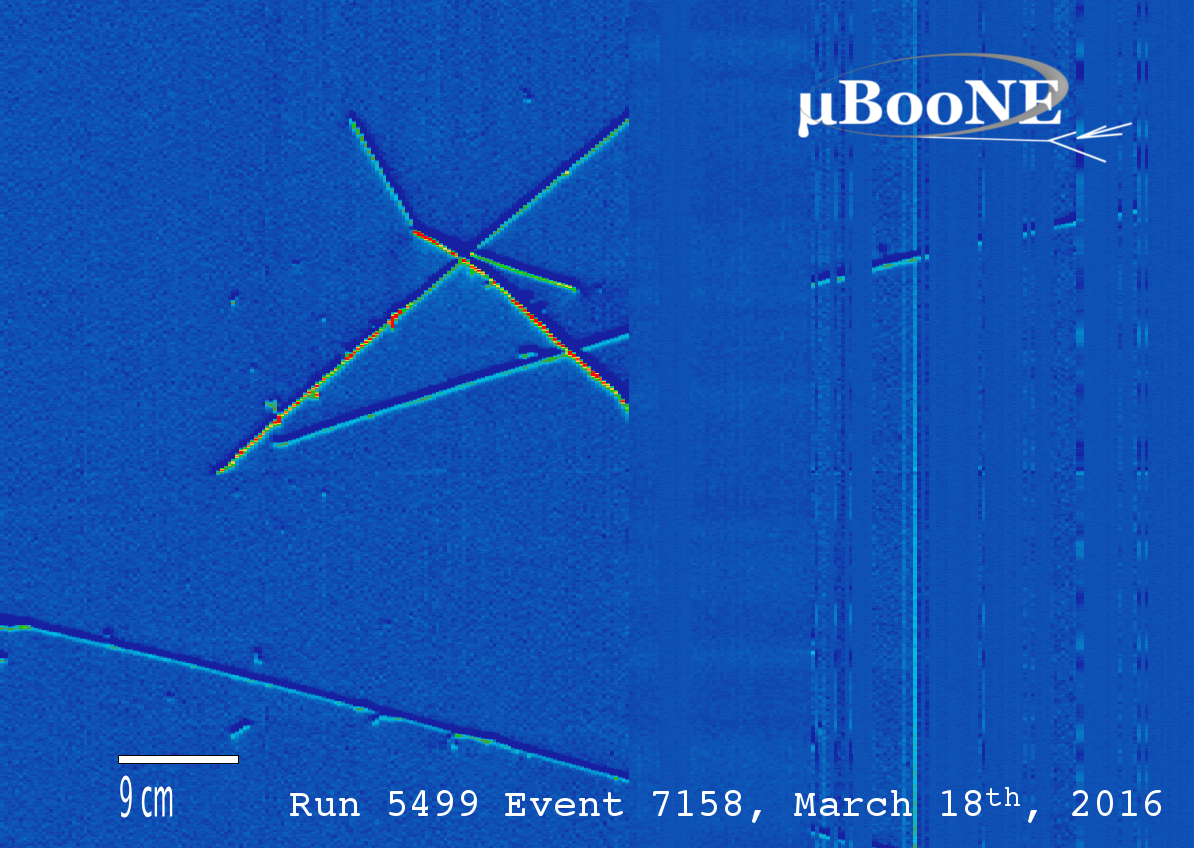
\includegraphics[width=0.5\textwidth + 1cm]{images/FirstCCInclusive/r5499_s143_ev7158/plane1.png}
   \label{fig:sel1_r5499_1}}
\subfloat[][Reconstructed 3D image (V plane projection)]
   {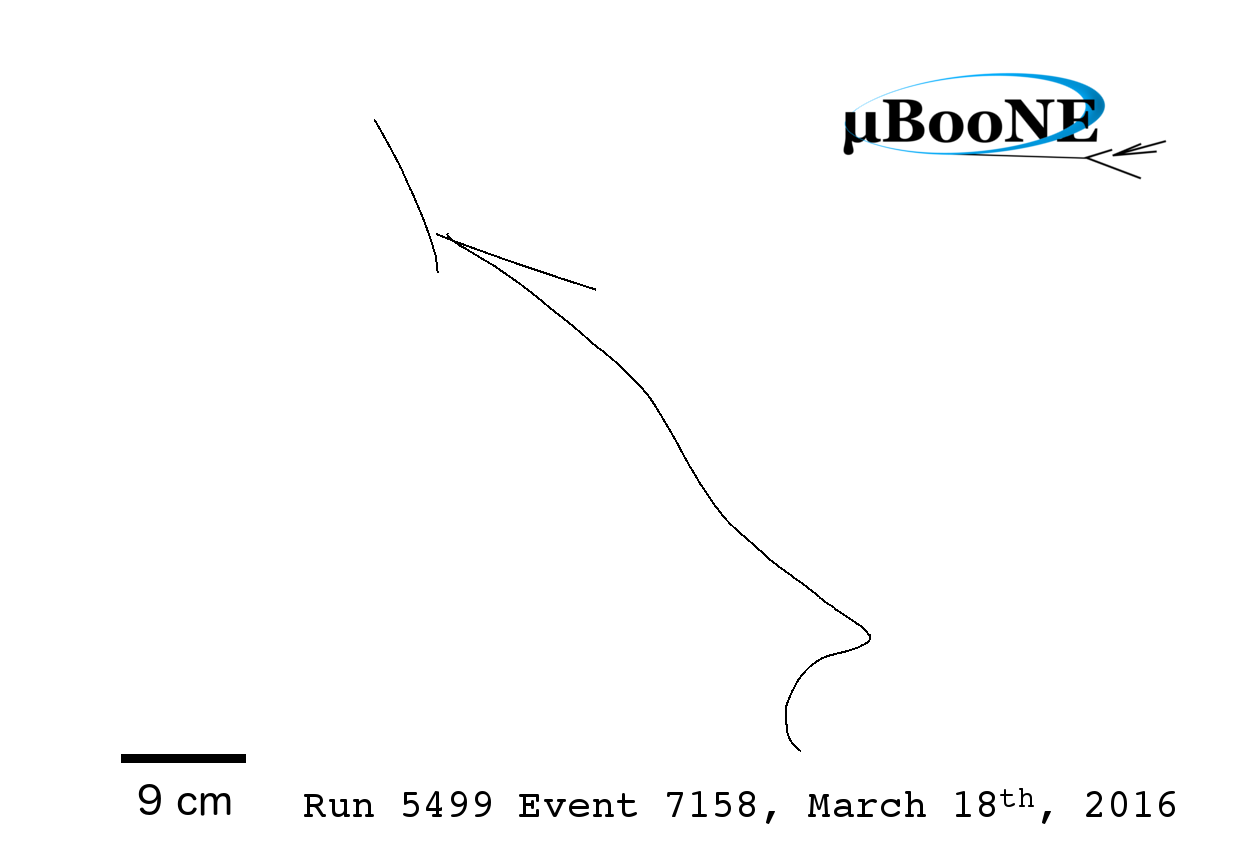
\includegraphics[width=0.5\textwidth + 1cm]{images/FirstCCInclusive/r5499_s143_ev7158/plane1_reco.png}
   \label{fig:sel1_r5499_1_reco}} \\   
\caption[Event View for Run 5499, Event 7158]{Event view for run 5499, event 7158, selected by this analysis. The plots on the left show the event view in all three wire planes. The Y and V plane show gaps of unresponsive wires and noise (see Figures \ref{fig:sel1_r5499_2} and \ref{fig:sel1_r5499_1}). The reconstruction successfully bridges these gaps. The plots on the right show the \gls{3d} reconstructed image projected onto each wire plane. The track reconstruction algorithm shown is pandoraNu. Note that some tracks visible on the left hand plots are missing on the right because they have been rejected in the cosmic removal pass. All figures have the same scale (indicated by the white bar in the bottom left) and aspect ratio. Sourced from \cite{MicroBooNECCInclPN}.}
\label{fig:sel1_r5499}
\end{adjustwidth}
\end{figure}

% TODO momentum axis label has to be shifted!

% \section{Unfolding}
% D'Agostini unfolding \cite{DAgostiniUnfolding}
